%
% Template Laporan Skripsi/Thesis Universitas Indonesia
%
% @author  Ichlasul Affan, Azhar Kurnia
% @version 2.2.1
%
% Dokumen ini dibuat berdasarkan standar IEEE dalam membuat class untuk
% LaTeX dan konfigurasi LaTeX yang digunakan Fahrurrozi Rahman ketika
% membuat laporan skripsi, yang kemudian diadaptasi oleh Andreas Febrian dan
% Lia Sadita untuk template skripsi tahun 2010.
% Konfigurasi template sebelumnya telah disesuaikan dengan
% aturan penulisan thesis yang dikeluarkan UI pada tahun 2017.
%


%
% Tipe dokumen adalah report dengan satu kolom.
%
\documentclass[12pt, a4paper, onecolumn, twoside, final]{report}
\raggedbottom

% Load konfigurasi LaTeX untuk tipe laporan thesis
\usepackage{_internals/uithesis}
%
\UseRawInputEncoding
% Load konfigurasi khusus untuk laporan yang sedang dibuat
\input{config/settings}
% Daftar pemenggalan suku kata dan istilah dalam LaTeX
\include{_internals/hypeindonesia}
% Daftar istilah yang mungkin perlu ditandai
%
% @author  Andreas Febrian
% @version 2.2.1
% @edit by Ichlasul Affan
%
% Mendaftar seluruh istilah yang mungkin akan perlu dijadikan
% italic atau bold pada setiap kemunculannya dalam dokumen.
%
% v2.2.1 - support untuk Glossary (daftar istilah)
%

% Istilah/alias yang tidak perlu dimasukkan ke dalam Glossary/Daftar Istiilah
\var{\license}{\f{Creative Common License 1.0 Generic}}
\var{\bslash}{$\setminus$}


\makeglossaries

% Contoh istilah
\newglossaryentry{latex}
{
	name=\LaTeX,
	description={Sebuah \f{mark up language} yang didesain khusus untuk karya tulis ilmiah}
}

% Contoh Akronim
\newacronym{pdf}{PDF}{\f{Portable Document Format}}


% Awal bagian penulisan laporan
\begin{document}

%
% Sampul Laporan
%
\include{_internals/sampul}
\ifodd\thechapterpagecount\forceclearchapter\fi


%
% Gunakan penomoran romawi untuk nomor halaman
%
\pagenumbering{roman}


%
% Halaman Judul Dalam
%
\strcompare{Kampus Merdeka}{\type}{} {
	\addtocontents{toc}{\protect\addvspace{-1em}}
	\addChapter{Halaman Judul}
	%
% Halaman Judul Laporan
%
% @author  unknown
% @version 2.2.0
% @edit by Andreas Febrian, Ichlasul Affan
%

\begin{titlepage}
	\begin{singlespace*}
	    \begin{center}
	    	\begin{figure}
	            \begin{center}
	                \includegraphics[width=2.5cm]{assets/pics/makara_kuning.png}
	            \end{center}
	        \end{figure}
	        \vspace*{-0.25cm}
	        \large
	        \bo{
	        	UNIVERSITAS INDONESIA\\
	        }
	
	        \vspace*{1.0cm}
	        % judul thesis harus dalam 14pt Times New Roman
	        \large
	        \bo{\Judul} \\[1.0cm]
	
	        \vspace*{2.5 cm}
	        % harus dalam 14pt Times New Roman
	        \large
	        \bo{\Type} \\[0.5cm]
	        % keterangan prasyarat
	        \normalsize
	        Diajukan sebagai salah satu syarat untuk memperoleh gelar \\
	        \gelar\\
	
			% Sesuaikan spacing agar semua informasi muat dalam satu halaman 
	        \vspace*{4 cm}
	        
	        % penulis dan npm
	        \large
	        \ifx\blank\npmDua
		        \bo{\PenulisSatu} \\
		        \bo{\npmSatu} \\
		    \else
		    	\bo{\PenulisSatu~/ \npmSatu~/ \ProgramSatu}\\
		    	\bo{\PenulisDua~/ \npmDua~/ \ProgramDua}\\
		    \fi
		    \ifx\blank\npmTiga\else
			    \bo{\PenulisTiga~/ \npmTiga~/ \ProgramTiga}\\
		    \fi
		    
			% Sesuaikan spacing agar semua informasi muat dalam satu halaman 
	        \vspace*{4.75 cm}
	
	        % informasi mengenai fakultas dan program studi
	        \large
	        \bo{
	        	FAKULTAS \Fakultas\\
	        	PROGRAM STUDI \ProgramSatu \\
	        	DEPOK \\
	        	\bulanTahun
	        }
	        \normalsize
	    \end{center}
	\end{singlespace*}
\end{titlepage}

	\ifodd\thechapterpagecount\forceclearchapter\thispagestyle{onlypage}\fi
}


%
% Halaman Orisinalitas
%
\strcompare{Laporan Kerja Praktik}{\type}{} {
\strcompare{Kampus Merdeka}{\type}{} {
	\addtocontents{toc}{\protect\addvspace{-1em}}
    \addChapter{Halaman Orisinalitas}
	\include{src/00-frontMatter/pernyataanOrisinalitas}
	\ifodd\thechapterpagecount\forceclearchapter\thispagestyle{onlypage}\fi
}}

% Memunculkan penomoran romawi untuk halaman-halaman awal
\pagenumbering{roman}


% Setelah bagian ini, halaman dihitung sebagai halaman ke 2 atau 3
\strcompare{Laporan Kerja Praktik}{\type}{\setcounter{page}{2}} {
	\strcompare{Kampus Merdeka}{\type}{\setcounter{page}{2}} {
		\setcounter{page}{3}
	}
}


%
% Lembar Pengesahan
%
\strcompare{Laporan Kerja Praktik}{\type}
{
	% Lembar Pengesahan Kerja Praktik dari LaTeX
	\addChapter{Lembar Persetujuan Dosen Kerja Praktik}
	\include{src/00-frontMatter/pengesahanKP}
	\ifodd\thechapterpagecount\forceclearchapter\thispagestyle{onlypage}\fi
}{
\strcompare{Kampus Merdeka}{\type}
{
	\addChapter{Lembar Pengesahan}
	\include{src/00-frontMatter/pengesahanMBKM}
	\ifodd\thechapterpagecount\forceclearchapter\thispagestyle{onlypage}\fi
}
{
	\addChapter{Lembar Pengesahan}
	% Gunakan salah satu (comment atau hapus kode yang tidak perlu):
	% Lembar Pengesahan Tugas Akhir dari LaTeX
	\strcompare{Doktor}{\jenjang}
	{\include{src/00-frontMatter/pengesahanSidangS3}}
	{\include{src/00-frontMatter/pengesahanSidang}}
	% Lembar Pengesahan dari PDF lain (misal: generated oleh SISIDANG [Fasilkom])
	%\putpdf{assets/pdfs/pengesahanSidang.pdf}
	\ifodd\thechapterpagecount\forceclearchapter\thispagestyle{onlypage}\fi
}}


\strcompare{Laporan Kerja Praktik}{\type}{} {
\strcompare{Kampus Merdeka}{\type}{} {
	%
	% Kata Pengantar
	%
	\addChapter{\kataPengantar}
	%-------------------------%
\pagestyle{onlypage}
\chapter*{\kataPengantar}
%-----------------------------------------------------------------------------%

Puji syukur kepada Tuhan Yang Maha Kuasa, karena di dalam penyertaan-Nya penelitian ini dapat dilaksanakan dan diselesaikan. Penulis tidak pernah lepas dari tuntunan-Nya dalam menyelesaikan laporan penelitian berjudul ``Pemantauan Kepatuhan secara Otomatis melalui Analisis Log pada Moodle Berbasis Kecerdasan Buatan'' ini.

Ucapan terima kasih secara khusus penulis sampaikan kepada Bapak Amril Syalim, S.Kom., M.Eng., Ph.D. yang telah membimbing proses penelitian ini dari awal hingga akhir. Segala masukan dan ilmu yang diberikan sangat berharga dan menjadi pertimbangan akademik dan karir penulis ke depannya.

Penelitian ini didukung oleh Computer Systems Lab (CSL) Fakultas Ilmu Komputer Universitas Indonesia yang telah mendukung pengembangan sistem ini. Ucapan terima kasih penulis sampaikan kepada Pak Maman dan Tim ITF yang telah mensupport akuisisi data dari awal penelitian. Dukungan teknis dan infrastruktur yang diberikan sangat membantu dalam proses pengumpulan dan analisis data log Moodle.

Terakhir, penulis mengucapkan terima kasih kepada Mama, Papa, Ivan, dan Irman yang telah memberikan dukungan tak terhingga sepanjang perjalanan akademik ini. Ucapan terima kasih juga penulis sampaikan kepada rekan-rekan ``Certified Gardener'' yang turut memberikan dukungan moral dan semangat dalam penyelesaian penelitian ini.

Penulis menyadari bahwa laporan \type~ini masih jauh dari sempurna. Oleh karena itu, apabila terdapat kesalahan atau kekurangan dalam laporan ini, penulis memohon agar kritik dan saran bisa disampaikan langsung melalui surel penulis (\texttt{yan.christofer@ui.ac.id}).


% Untuk input gambar tanda tangan, silahkan sesuaikan xshift, yshift, dan width dengan gambar tanda tangan Anda
%\begin{tikzpicture}[remember picture,overlay,shift={(current page.north east)}]
%\node[anchor=north east,xshift=-3cm,yshift=-6.2cm]{\includegraphics[width=3cm]{assets/pics/tanda_tangan_wikipedia.png}};
%\end{tikzpicture}

\vspace*{0.1cm}
\begin{flushright}
Depok, \tanggalSiapSidang\\[0.1cm]
\ifx\blank\npmDua
	\vspace*{1.5cm}
	\penulisSatu
\else
	Tim Penulis
\fi

\end{flushright}

	\ifodd\thechapterpagecount\forceclearchapter\thispagestyle{onlypage}\fi

	%
	% Lembar Persetujuan Publikasi Ilmiah
	%
	\addChapter{Lembar Persetujuan Karya Ilmiah}
	\include{src/00-frontMatter/persetujuanPublikasi}
	\ifodd\thechapterpagecount\forceclearchapter\thispagestyle{onlypage}\fi
}}


%
% Untuk halaman pertama setiap chapter mulai dari abstrak, tetap berikan mark universitas.
%
\pagestyle{first-pages}


%
% Abstrak
%
\addChapter{Abstrak}
%
% Halaman Abstrak
%
% @author  Andreas Febrian
% @version 2.2.0
% @edit by Ichlasul Affan
%

\chapter*{Abstrak}
\singlespacing

\noindent \begin{tabular}{l l p{10cm}}
	\ifx\blank\npmDua
		Nama&: & \penulisSatu \\
		Program Studi&: & \programSatu \\
	\else
		Nama Penulis 1 / Program Studi&: & \penulisSatu~/ \programSatu\\
		Nama Penulis 2 / Program Studi&: & \penulisDua~/ \programDua\\
	\fi
	\ifx\blank\npmTiga\else
		Nama Penulis 3 / Program Studi&: & \penulisTiga~/ \programTiga\\
	\fi
	Judul&: & \judul \\
	Pembimbing&: & \pembimbingSatu \\
	\ifx\blank\pembimbingDua
    \else
        \ &\ & \pembimbingDua \\
    \fi
    \ifx\blank\pembimbingTiga
    \else
    	\ &\ & \pembimbingTiga \\
    \fi
\end{tabular} \\

\vspace*{0.5cm}

\noindent
Dalam rangka memperkuat integritas akademik pada pembelajaran era digital, penelitian ini mengembangkan sistem deteksi kecurangan yang lebih komprehensif berbasis \textit{machine learning}. Dengan memanfaatkan data log yang kaya dan terstruktur dari Moodle, sistem mengintegrasikan beragam teknik analitik yang mencakup \textbf{deteksi anomali}, \textbf{clustering}, dan \textbf{pembelajaran terawasi} menggunakan model \textit{advanced ensemble}. Berbagai \textit{similarity matrix} (seperti \textit{navigation}, \textit{timing}, dan \textit{answer similarity}) dikombinasikan untuk menghasilkan fitur-fitur baru yang mampu menggali pola perilaku mencurigakan. Selain itu, penerapan \textbf{gradient boosting}, \textbf{neural network}, hingga \textbf{one-class SVM} dan \textbf{ensemble threshold optimization} memberikan kemampuan deteksi kecurangan yang lebih akurat. Hasil evaluasi menunjukkan bahwa metode gabungan ini mampu meningkatkan sensitivitas dan spesifisitas dalam mengungkap potensi kecurangan secara proaktif, sehingga dapat menjadi landasan yang efektif bagi institusi pendidikan dalam mengurangi praktik kecurangan serta memastikan kepatuhan pengguna di platform Moodle.

\vspace*{0.2cm}

\noindent Kata kunci: \\
\f{Moodle, LMS, Log Aktivitas, Pembelajaran Mesin, Deteksi Anomali, Ensemble Methods, Threshold Optimization, Integritas Akademik} \\

\setstretch{1.4}
\newpage


%
% Halaman Abstract
%
% @author  Andreas Febrian
% @version 2.2.0
% @edit by Ichlasul Affan
%

\chapter*{ABSTRACT}
\singlespacing

\noindent \begin{tabular}{l l p{11.0cm}}
	\ifx\blank\npmDua
		Name&: & \penulisSatu \\
		Study Program&: & \studyProgramSatu \\
	\else
		Writer 1 / Study Program&: & \penulisSatu~/ \studyProgramSatu\\
		Writer 2 / Study Program&: & \penulisDua~/ \studyProgramDua\\
	\fi
	\ifx\blank\npmTiga\else
		Writer 3 / Study Program&: & \penulisTiga~/ \studyProgramTiga\\
	\fi
	Title&: & \judulInggris \\
	Counselor&: & \pembimbingSatu \\
	\ifx\blank\pembimbingDua
    \else
        \ &\ & \pembimbingDua \\
    \fi
    \ifx\blank\pembimbingTiga
    \else
    	\ &\ & \pembimbingTiga \\
    \fi
\end{tabular} \\

\vspace*{0.5cm}

\noindent
In order to strengthen academic integrity in the digital learning era, this study develops a more comprehensive cheating detection system based on machine learning. By utilizing rich and structured log data from Moodle, our system integrates multiple analytical techniques including anomaly detection, clustering, and supervised learning through advanced ensemble models. Various similarity matrices (such as navigation, timing, and answer similarity) are combined to generate new features that uncover potentially suspicious behavior patterns. In addition, the application of gradient boosting, neural network, one-class SVM, and ensemble threshold optimization provides more accurate cheating detection capabilities. Evaluation results show that this combined method enhances both sensitivity and specificity in proactively revealing potential cheating incidents, making it an effective foundation for educational institutions to minimize dishonest practices and ensure user compliance within the Moodle platform.

\vspace*{0.2cm}

\noindent Key words: \\
Moodle, LMS, Activity Logs, Machine Learning, Anomaly Detection, Ensemble Methods, Threshold Optimization, Academic Integrity \\

\setstretch{1.4}
\newpage



%
% Daftar Isi, Gambar, dan Tabel
%

\addDefaultListPage{\tableofcontents}
\addDefaultListPage{\listoffigures}
\addDefaultListPage{\listoftables}


%
% Daftar Kode Program
% Jika tidak digunakan, commment kode ini.
%
\addCustomListPage{\listoflistings}{\lstlistlistingname}


%
% Daftar Equation (Persamaan Matematis)
% Jika bagian ini diperlukan, uncomment kode ini.
%
% \addCustomListPage{\listofequ}{\listofequname}


%
% Daftar Isi yang Didefinisikan Sendiri (Custom)
% Definisi jenis objek baru dapat dilakukan di uithesis.sty
%
% \addCustomListPage{\listofthing}{\listofthingname}


%
% Daftar Lampiran
% Jika tidak digunakan, commment kode ini.
%
%\addCustomListPage{\listofappendix}{\listofappendixname}


% Kembalikan pengaturan chapter dan daftar isi ke aturan awal mulai dari halaman ini
\noCAPinToC
\ifodd\thechapterpagecount\clearpage\else\forceclearchapter\fi

% Jika penomoran romawi selesai di ganjil
% \naiveoddclearchapter
% Jika penomoran romawi selesai di genap
% \naiveevenclearchapter


%
% Gunakan penomoran Arab (1, 2, 3, ...) setelah bagian ini.
%
\pagenumbering{arabic}
\pagestyle{standard}


%
% Isi dari Tugas Akhir/Karya Ilmiah
%
\setoddevenheader
%-----------------------------------------------------------------------------%
\chapter{\babSatu}
\label{bab:1}
%-----------------------------------------------------------------------------%
Pada bab ini, akan dijelaskan tentang topik penelitian, termasuk di dalamnya latar belakang dan permasalahan yang diselesaikan pada penelitian ini. 

%-----------------------------------------------------------------------------%
\section{Latar Belakang}
\label{sec:latarBelakang}
%-----------------------------------------------------------------------------%

Era digital mendorong transformasi pendidikan tinggi secara pesat, terutama sejak pandemi COVID-19. Institusi perguruan tinggi berbondong-bondong mengadopsi \textit{Learning Management System} (LMS) seperti Moodle untuk mendukung pembelajaran daring dan pelaksanaan ujian jarak jauh \cite{Yulita2023}. Digitalisasi ini membawa manfaat dalam hal fleksibilitas dan jangkauan, namun juga menimbulkan tantangan baru terhadap integritas akademik. Menjaga kejujuran akademik di lingkungan pembelajaran daring kini menjadi isu krusial, karena proses evaluasi yang berpindah ke ranah online rentan disalahgunakan untuk melakukan kecurangan \cite{Kamalov2021}.

Studi menunjukkan bahwa risiko kecurangan akademik cenderung meningkat dalam konteks pembelajaran daring. Lanier menemukan tingkat kecurangan yang jauh lebih tinggi pada kelas jarak jauh dibanding kelas tatap muka tradisional \cite{Lanier2006}. Sementara itu, survei terhadap mahasiswa dan dosen di Norwegia mengidentifikasi enam modus kecurangan paling umum dalam ujian daring, seperti peniruan identitas, penggunaan bahan terlarang, dan kolaborasi tidak sah \cite{Chirumamilla2020}.

Dalam konteks ini, data log aktivitas Moodle menjadi sumber informasi yang sangat berharga. Moodle secara otomatis merekam jejak interaksi pengguna secara terstruktur, mencakup waktu akses, pola navigasi, durasi pengerjaan soal, hingga kesamaan jawaban antar peserta. Analisis mendalam terhadap log ini berpotensi mengungkap berbagai pola perilaku yang mengindikasikan kecurangan, seperti kolaborasi tidak sah yang terdeteksi dari kesamaan pola navigasi dan jawaban \cite{Murdoch2019}, serta berbagai anomali perilaku selama pandemi \cite{Balderas2020}.

Pendekatan konvensional untuk mendeteksi kecurangan umumnya mengandalkan pemeriksaan manual atau sistem berbasis aturan sederhana. Namun, metode ini memiliki keterbatasan serius, seperti skalabilitas rendah dan kecenderungan menghasilkan \textit{false positives} \cite{MorenoMarcos2023}. 

Sebagai solusi, penelitian ini mengusulkan pendekatan berbasis \textit{machine learning} yang mengintegrasikan beragam teknik analitik. Kerangka kerja yang dikembangkan berfokus pada model pembelajaran terawasi (\textit{supervised learning}) seperti \textit{Gradient Boosting}, \textit{Random Forest}, dan \textit{Neural Network}, yang diperkuat dengan metode deteksi anomali seperti \textit{Isolation Forest} dan \textit{Local Outlier Factor} sebagai teknik komplementer. Pendekatan ensemble ini dilengkapi dengan analisis matriks kesamaan (\textit{similarity matrices}) yang mencakup pola navigasi, waktu pengerjaan, dan jawaban mahasiswa, serta optimasi ambang batas (\textit{threshold optimization}) untuk meningkatkan akurasi deteksi.

Integrasi berbagai teknik ini memungkinkan sistem mengenali pola-pola mencurigakan dengan lebih akurat, seperti yang ditunjukkan dalam penelitian sebelumnya menggunakan data MOOC \cite{Alexandron2019}. Penggunaan matriks kesamaan dan analisis graf juga terbukti efektif dalam mengungkap kolusi antar mahasiswa \cite{Chang2023}. Dengan demikian, penelitian ini berkontribusi pada pengembangan sistem deteksi kecurangan yang lebih komprehensif dan adaptif untuk platform Moodle.

%-----------------------------------------------------------------------------%
\section{Permasalahan}
\label{sec:masalah}
%-----------------------------------------------------------------------------%

Kecurangan akademik merupakan permasalahan serius di institusi pendidikan tinggi karena dapat merusak integritas dan kualitas hasil pembelajaran. Dalam konteks pembelajaran \textit{e-learning} menggunakan platform Moodle, potensi terjadinya kecurangan akademik semakin tinggi seiring dengan meningkatnya penggunaan ujian daring dan tugas online. Beragam bentuk kecurangan dapat terjadi, misalnya kolusi antar mahasiswa untuk berbagi jawaban, penyalahgunaan akun, atau penggunaan sumber tidak sah selama ujian.

Kompleksitas permasalahan ini menuntut pendekatan deteksi yang lebih canggih, yang tidak hanya mengandalkan satu metode, melainkan mengintegrasikan berbagai teknik analitik untuk menghasilkan deteksi yang lebih akurat dan dapat diandalkan. Diperlukan juga kemampuan untuk menganalisis berbagai aspek perilaku pengguna secara simultan, dari pola navigasi hingga kesamaan jawaban, serta mengoptimalkan parameter deteksi untuk meminimalkan kesalahan klasifikasi.

%-----------------------------------------------------------------------------%
\subsection{Pertanyaan Penelitian}
\label{sec:definisiMasalah}
%-----------------------------------------------------------------------------%
Berdasarkan permasalahan yang telah diuraikan, penelitian ini berusaha menjawab pertanyaan-pertanyaan berikut:
\begin{enumerate}
    \item Bagaimana mengembangkan pendekatan berbasis pembelajaran mesin yang efektif untuk mendeteksi potensi kecurangan akademik dalam pembelajaran daring menggunakan data log aktivitas Moodle?
    \item Sejauh mana integrasi berbagai teknik analisis data dapat meningkatkan akurasi dan reliabilitas deteksi perilaku mencurigakan dalam konteks pembelajaran daring?
    \item Bagaimana karakteristik dan pola perilaku pengguna yang teridentifikasi dari hasil analisis dapat memberikan wawasan untuk meningkatkan integritas akademik dalam pembelajaran daring?
\end{enumerate}

%-----------------------------------------------------------------------------%
\subsection{Batasan Penelitian}
\label{sec:batasanMasalah}
%-----------------------------------------------------------------------------%
Untuk memastikan penelitian ini tetap terfokus dan terarah, beberapa batasan dan ruang lingkup berikut diterapkan:
\begin{enumerate}
    \item Lingkup Data: Data yang digunakan dalam penelitian ini dibatasi pada log aktivitas pengguna dari platform Moodle di lingkungan Fasilkom UI,dengan model dilatih menggunakan data artifisial yang karakteristiknya divalidasi terhadap data riil, dan kemudian diterapkan pada data log riil Fasilkom UI untuk analisis.
    \item Jenis Kecurangan: Deteksi difokuskan pada pola perilaku mencurigakan yang tercermin dalam log aktivitas, matriks kesamaan, dan interaksi antar pengguna.
    \item Metode dan Algoritma: Pendekatan utama menggunakan model pembelajaran terawasi dengan ensemble, didukung metode deteksi anomali sebagai komplemen.
    \item Mode Implementasi: Sistem deteksi diimplementasikan dalam modus \textit{offline} untuk analisis retrospektif.
    \item Evaluasi: Kinerja sistem dievaluasi menggunakan metrik standar seperti presisi, sensitivitas, dan skor F1.
\end{enumerate}

%-----------------------------------------------------------------------------%
\section{Tujuan Penelitian}
\label{sec:tujuan}
%-----------------------------------------------------------------------------%
Penelitian ini memiliki tujuan utama untuk mengembangkan sistem deteksi kecurangan yang komprehensif berbasis analisis log aktivitas Moodle. Secara terperinci, tujuan penelitian ini adalah:
\begin{enumerate}
    \item Merancang dan mengimplementasikan kerangka kerja deteksi yang mengintegrasikan model pembelajaran terawasi dengan ensemble, didukung metode deteksi anomali, analisis matriks kesamaan, dan optimasi ambang batas.
    \item Mengembangkan dan mengevaluasi fitur-fitur baru berbasis matriks kesamaan untuk meningkatkan akurasi deteksi.
    \item Melakukan pengujian menyeluruh terhadap kinerja sistem menggunakan data log Moodle Fasilkom UI.
    \item Menganalisis dan menginterpretasikan pola-pola perilaku mencurigakan yang terdeteksi untuk mendukung upaya pencegahan kecurangan.
\end{enumerate}

%-----------------------------------------------------------------------------%
\section{Manfaat Penelitian}
\label{sec:manfaat}
%-----------------------------------------------------------------------------%
Penelitian ini diharapkan memberikan manfaat baik secara teoretis maupun praktis:
\begin{enumerate}
    \item Manfaat Teoretis:
    \begin{enumerate}
        \item Kontribusi pada pengembangan metode deteksi kecurangan berbasis ensemble.
        \item Pemahaman baru tentang efektivitas matriks kesamaan dalam analisis perilaku.
        \item Landasan metodologis untuk penelitian lanjutan.
    \end{enumerate}
    
    \item Manfaat Praktis:
    \begin{enumerate}
        \item Sistem deteksi dini yang lebih akurat untuk institusi pendidikan.
        \item Dukungan objektif untuk pengambilan keputusan terkait integritas akademik.
        \item Peningkatan efektivitas monitoring pembelajaran daring.
        \item Dasar pengembangan sistem deteksi real-time di masa depan.
    \end{enumerate}
\end{enumerate}

%-----------------------------------------------------------------------------%
\section{Langkah Penelitian}
\label{sec:langkahPenelitian}
%-----------------------------------------------------------------------------%

Berikut ini adalah langkah penelitian yang dilakukan:

\begin{enumerate}
\item \textbf{Tinjauan Literatur}\\
Mengkaji teori dan penelitian terkait deteksi kecurangan, metode ensemble, dan analisis matriks kesamaan dalam konteks pembelajaran daring.

\item \textbf{Pengumpulan dan Pengolahan Data}\\
Mengumpulkan log aktivitas Moodle, melakukan pembersihan data, dan mengekstraksi fitur-fitur relevan termasuk matriks kesamaan.

\item \textbf{Pengembangan Sistem}\\
Mengimplementasikan kerangka kerja deteksi yang mengintegrasikan model pembelajaran terawasi (\textit{Gradient Boosting}, \textit{Random Forest}, \textit{Neural Network}) sebagai komponen utama, diperkaya dengan metode deteksi anomali, analisis matriks kesamaan, dan optimasi ambang batas.

\item \textbf{Evaluasi dan Analisis}\\
Menguji kinerja sistem menggunakan metrik standar, menganalisis pola-pola yang terdeteksi, dan menginterpretasikan implikasinya.

\item \textbf{Penarikan Kesimpulan}\\
Menyimpulkan efektivitas pendekatan yang diusulkan dan merumuskan rekomendasi untuk pengembangan sistem dan penelitian lanjutan.
\end{enumerate}

%-----------------------------------------------------------------------------%
\section{Sistematika Penulisan}
\label{sec:sistematikaPenulisan}
%-----------------------------------------------------------------------------%

Sistematika penulisan laporan penelitian ini adalah sebagai berikut:

\begin{itemize}
\item \textbf{Bab 1 Pendahuluan}\\
Berisi latar belakang penelitian, perumusan masalah, batasan penelitian, tujuan penelitian, manfaat penelitian, langkah-langkah penelitian, serta sistematika penulisan.

\item \textbf{Bab 2 Landasan Teori dan Studi Literatur}\\
Mengkaji konsep-konsep fundamental tentang integritas akademik dalam pembelajaran daring, teknik-teknik pembelajaran mesin untuk deteksi anomali, serta penelitian-penelitian terkait dalam bidang analisis perilaku pengguna sistem pembelajaran daring.

\item \textbf{Bab 3 Metodologi dan Rancangan Sistem}\\
Menjelaskan pendekatan metodologis yang digunakan, termasuk desain sistem deteksi, proses pengolahan data, pemilihan dan integrasi metode analisis, serta kerangka evaluasi yang diterapkan.

\item \textbf{Bab 4 Implementasi dan Hasil Eksperimen}\\
Memaparkan implementasi sistem yang dikembangkan, hasil eksperimen yang dilakukan, serta analisis kinerja berdasarkan berbagai metrik evaluasi.

\item \textbf{Bab 5 Analisis dan Pembahasan}\\
Menganalisis secara mendalam temuan-temuan penelitian, interpretasi pola perilaku yang terdeteksi, serta implikasinya terhadap praktik pembelajaran daring.

\item \textbf{Bab 6 Kesimpulan dan Saran}\\
Menyajikan kesimpulan penelitian, kontribusi yang dihasilkan, keterbatasan yang ditemui, serta rekomendasi untuk pengembangan dan penelitian lanjutan.
\end{itemize}


\clearchapter
%-----------------------------------------------------------------------------%
\chapter{\babDua}
\label{bab:2}
%-----------------------------------------------------------------------------%
\todo{
	Bab ini, biasanya namanya adalah "Studi Literatur" atau "Tinjauan Pustaka".
	Akan tetapi, beberapa fakultas atau dosen pembimbing meminta Bab 2 untuk dinamakan lain, seperti "Kerangka Berpikir".
}

Untuk memulai penelitian, dibutuhkan kerangka berpikir yang sesuai untuk permasalahan yang ingin dipecahkan.
Untuk membentuk kerangka berpikir yang sesuai, perlu dikaitkan dengan hasil studi literatur yang telah dilakukan.
Oleh karena itu, pada bab ini, akan dijelaskan hasil studi literatur yang telah dilakukan yang telah dikaitan dengan kerangka kerja untuk penelitian ini.


%-----------------------------------------------------------------------------%
\section{Apa itu \latex?}
\label{sec:latex}
%-----------------------------------------------------------------------------%

%-----------------------------------------------------------------------------%
\subsection{\latex~Secara Singkat}
\label{sec:latexBrief}
%-----------------------------------------------------------------------------%
Berdasarkan \cite{latex:intro}: \\
\begin{tabular}{| p{14cm} |}
	\hline
	\gls{latex} is a family of programs designed to produce publication-quality typeset documents.
	It is particularly strong when working with mathematical symbols. \\
	The history of \gls{latex} begins with a program called TEX.
	In 1978, a computer scientist by the name of Donald Knuth grew frustrated with the mistakes that his publishers made in typesetting his work.
	He decided to create a typesetting program that everyone could easily use to typeset documents, particularly those that include formulae, and made it freely available.
	The result is TEX. \\
	Knuth's product is an immensely powerful program, but one that does focus very much on small details.
	A mathematician and computer scientist by the name of Leslie Lamport wrote a variant of TEX called \gls{latex} that focuses on document structure rather than such details. \\
	\hline
\end{tabular}

\vspace*{0.2cm}

Dokumen \gls{latex}~sangat mudah, seperti halnya membuat dokumen teks biasa.
Ada beberapa perintah yang diawali dengan tanda '\bslash'.
Seperti perintah \code{\bslash\bslash}~yang digunakan untuk memberi baris baru.
Perintah tersebut juga sama dengan perintah \code{\bslash{}newline}.
Pada bagian ini akan sedikit dijelaskan cara manipulasi teks dan perintah-perintah \gls{latex}~yang mungkin akan sering digunakan.
Jika ingin belajar hal-hal dasar mengenai \gls{latex}, silakan kunjungi:

\begin{itemize}
	\item \url{http://frodo.elon.edu/tutorial/tutorial/}, atau
	\item \url{http://www.maths.tcd.ie/~dwilkins/LaTeXPrimer/}
\end{itemize}

%-----------------------------------------------------------------------------%
\subsection{\latex~Kompiler dan IDE}
\label{sec:latexCompiler}
%-----------------------------------------------------------------------------%
Untuk menggunakan \gls{latex}~(pada konteks hanya sebagai pengguna), tidak perlu banyak tahu mengenai hal-hal didalamnya.
Dengan menggunakan \f{Integrated Development Environment} (IDE), penggunaan \gls{latex}~akan serupa dengan pembuatan dokumen secara visual, layaknya OpenOffice Writer atau Microsoft Word.
Orang-orang yang menggunakan \gls{latex}~relatif lebih teliti dan terstruktur mengenai cara penulisan yang dia gunakan, karena \gls{latex}~memaksa untuk seperti itu.

Untuk mencoba \gls{latex}, diperlukan kompiler dan IDE.
Bagi pengguna Microsoft Windows dan Mac OS, instalasi kompiler \gls{latex}~dapat menggunakan MikTeX (\url{https://miktex.org/download}).
Bagi pengguna Linux, instalasi kompiler \gls{latex}~dapat menggunakan Texlive ( \url{http://www.tug.org/texlive/}).
Distro-distro \f{mainstream} di Linux seperti Ubuntu biasanya telah menyediakan \f{package} \code{texlive} melalui \f{package manager}.
Apabila ingin melakukan instalasi Texlive melalui \f{package manager}, lakukan instalasi package \code{texlive-full} atau setidaknya \code{texlive-science} agar prasyarat \f{template} ini tersedia secara lengkap.

Beberapa text editor atau IDE yang dapat digunakan adalah sebagai berikut:
\begin{itemize}
	\item \underline{\href{https://www.texstudio.org/}{TeXstudio}} (direkomendasikan),
	\item TeXWorks (biasanya bawaan dari \underline{\href{https://miktex.org/download}{MikTeX}}),
	\item \underline{\href{http://www.xm1math.net/texmaker/}{Texmaker}}, atau
	\item Microsoft Visual Studio Code, dengan \f{plugin} \underline{\href{https://marketplace.visualstudio.com/items?itemName=James-Yu.latex-workshop}{\gls{latex} Workshop}}.
	Untuk menggunakan \f{plugin} tersebut, diperlukan instalasi MikTeX dan Perl.
	Alternatif lain untuk persyaratan tersebut adalah menggunakan \f{plugin} Remote - WSL jika memiliki distro Windows Subsystem for Linux (WSL) 2 yang sudah terpasang \code{texlive}.
\end{itemize}


%-----------------------------------------------------------------------------%
\section{\f{Formatting} Teks Dasar}
\label{sec:latexBasicFormatting}
%-----------------------------------------------------------------------------%
Hal pertama yang mungkin ditanyakan adalah bagaimana membuat huruf tercetak tebal, miring, atau memiliki garis bawah.
Pada Texmaker, Anda bisa melakukan hal ini seperti halnya saat mengubah dokumen dengan OO Writer.
Namun jika tetap masih tertarik dengan cara lain, ini dia:

\begin{itemize}
	\item \bo{Bold} \\
	Gunakan perintah \code{\bslash{}textbf$\lbrace\rbrace$} atau
	\code{\bslash{}bo$\lbrace\rbrace$}.\\
	Contoh: \textbf{Contoh hasil tulisan} atau \bo{Contoh hasil tulisan}.
	\item \f{Italic} \\
	Gunakan perintah \code{\bslash{}textit$\lbrace\rbrace$} atau
	\code{\bslash{}f$\lbrace\rbrace$}.\\
	Contoh: \textit{Contoh hasil tulisan} atau \f{Contoh hasil tulisan}.
	\item \underline{Underline} \\
	Gunakan perintah \code{\bslash{}underline$\lbrace\rbrace$}.\\
	Contoh: \underline{Contoh hasil tulisan}.
	\item $\overline{Overline}$ \\
	Gunakan perintah \code{\$\bslash{}overline\$}.\\
	Contoh: $\overline{Contoh~hasil~tulisan}$.
	\item $^{superscript}$ \\
	Gunakan perintah \code{\$\bslash{}$\lbrace\rbrace$\$}.\\
	Contoh: $^{Contoh~hasil~tulisan}$.
	\item $_{subscript}$ \\
	Gunakan perintah \code{\$\bslash{}\_$\lbrace\rbrace$\$}.\\
	Contoh: $_{Contoh~hasil~tulisan}$.
\end{itemize}

% v2.2.1: tutorial dipindah dari Bab 3 ke Bab 2
Ada beberapa hal lain yang bisa digunakan.
\begin{itemize}
	\item Kombinasi \bo{Bold} dan \f{Italic}: \\
	Gunakan perintah \code{\bslash{}bi$\lbrace\rbrace$}. \\
	Contoh: \bi{Contoh hasil tulisan}.
	\item Menebalkan teks formula matematis: \\
	Gunakan perintah \code{\bslash{}m$\lbrace\rbrace$}. \\
	Contoh: \m{\alpha~\beta}
	\item Menebalkan teks formula matematis, sekaligus meletakkannya di tengah: \\
	Gunakan perintah \code{\bslash{}mc$\lbrace\rbrace$}. \\
	Contoh: \mc{\alpha~\beta}
	\item Menggunakan \f{monospaced font} untuk kode:
	Gunakan perintah \code{\bslash{}texttt$\lbrace\rbrace$} atau \code{\bslash{}code$\lbrace\rbrace$}. \\
	Contoh: \texttt{Contoh hasil tulisan} atau \code{Contoh hasil tulisan}.
\end{itemize}

Perintah \code{\bslash{}f}, \code{\bslash{}bo}, \code{\bslash{}bi}, \code{\bslash{}m}, \code{\bslash{}mc},
dan \code{\bslash{}code} hanya dapat digunakan jika package \code{\_internals/uithesis} digunakan.

%-----------------------------------------------------------------------------%
\section{Memasukan Gambar}
\label{sec:latexImage}
%-----------------------------------------------------------------------------%
Setiap gambar dapat diberikan caption dan diberikan label. Label dapat digunakan untuk menunjuk gambar tertentu.
Jika posisi gambar berubah, maka nomor gambar juga akan diubah secara otomatis.
Begitu juga dengan seluruh referensi yang menunjuk pada gambar tersebut.
Contoh sederhana adalah \pic~\ref{fig:testGambar}, yang bisa dibuat dengan menggunakan \lst~\ref{code:latexImage}.
Harap diingat pada aturan Tugas Akhir UI, caption harus selalu \b{diletakkan di bawah gambar}.

\lstinputlisting[language={[latex]tex}, caption=Contoh penggunaan gambar, label=code:latexImage]{assets/codes/tutorial/2-basicFigure.tex}

Berikut adalah penjelasan dari \lst~\ref{code:latexImage}:
\begin{itemize}
	\item Baris ke-2: \code{\bslash{}centering} digunakan untuk membuat gambar berada di tengah.
	\item Baris ke-3 dan 4: \code{\bslash{}includegraphics} digunakan untuk memasukkan gambar. \\
	\code{width=0.25\bslash{}textwidth} digunakan untuk mengatur lebar gambar sebesar 25\% dari lebar teks (dari ujung marjin kiri ke ujung marjin kanan).
	\item Baris ke-5: \code{\bslash{}caption} digunakan untuk memberikan \f{caption} pada gambar.
	\f{Caption} tersebut diletakkan setelah \code{includegraphics} agar \f{caption} berada di bawah gambar.
	\item Baris ke-6: \code{\bslash{}label} digunakan untuk memberikan label pada gambar.
	Label ini bisa digunakan di suatu paragraf untuk merujuk pada gambar tersebut,
	dengan cara menuliskan \code{\bslash{}ref\{label\}} pada paragraf.
\end{itemize}

\begin{figure}
	\centering
	\includegraphics[width=0.25\textwidth]
	{assets/pics/makara_kuning.png}
	\caption{Makara Universitas Indonesia}
	\label{fig:testGambar}
\end{figure}


Anda juga bisa memasukkan sitasi atau URL sumber gambar, jika gambar tersebut bukan Anda sendiri yang membuatnya.
Contoh sederhana adalah \pic~\ref{fig:testGambarBersumber}, yang bisa dibuat dengan menggunakan \lst~\ref{code:latexImageSource}.

\lstinputlisting[language={[latex]tex}, caption=Contoh penggunaan gambar bersumber, label=code:latexImageSource]{assets/codes/tutorial/2-sourcedFigure.tex}

Pada baris ke-5, \code{\bslash{}captionsource} digunakan untuk memberikan caption dan sumber gambar.
Dalam kasus ini, sumber gambar merupakan sebuah URL, sehingga ditandai dengan perintah \code{\bslash{}url\{\}}.
Jika sumber gambar merupakan sebuah buku, jurnal, atau dokumen, maka bisa dilakukan sitasi menggunakan perintah \code{\bslash{}cite\{\}}.
Contoh: \code{\bslash{}captionsource\{Sesuatu\}\{\bslash{}cite\{latex:intro\}\}}.

\begin{figure}
	\centering
	\includegraphics[width=0.50\textwidth]
	{assets/pics/creative_commons.png}
	\captionsource{\license.}{{\url{https://creativecommons.org/licenses/by-nc-sa/1.0/}}}
	\label{fig:testGambarBersumber}
\end{figure}



%-----------------------------------------------------------------------------%
\section{Membuat Tabel}
\label{sec:latexTable}
%-----------------------------------------------------------------------------%
Tabel pada \gls{latex} dapat dibuat secara visual dengan bantuan \f{website} seperti \url{https://www.tablesgenerator.com/}.
Dengan menggunakan \textit{website} ini, maka pembuatan tabel akan menjadi lebih mudah.
\textit{User interface} dari \f{website} dapat dilihat pada Gambar \ref{fig:tablesgenerator}.

\begin{figure}
	\centering
	\includegraphics[width=0.5\textwidth]{assets/pics/tablesgenerator-dot-com.png}
	\caption{\textit{User interface} dari \textit{website} https://www.tablesgenerator.com/}
	\label{fig:tablesgenerator}
\end{figure}

Di sisi lain, tabel juga dapat diberi label dan caption seperti pada gambar.
Caption pada tabel terletak pada bagian atas tabel.
Contoh kode yang menyusun suatu tabel sederhana dapat dilihat pada \lst~\ref{code:latexTable}.

\lstinputlisting[language={[latex]tex}, caption=Contoh penggunaan tabel, label=code:latexTable]{assets/codes/tutorial/2-basicTable.tex}

Berikut adalah penjelasan dari \lst~\ref{code:latexTable}:
\begin{itemize}
	\item Baris ke-2: \code{\bslash{}centering} digunakan untuk membuat tabel berada di tengah.
	\item Baris ke-3: \code{\bslash{}caption} digunakan untuk memberikan \f{caption} pada tabel.
	\f{Caption} tersebut diletakkan setelah \code{begin\{tabular\}} agar \f{caption} berada di atas tabel.
	\item Pada baris ke-3, terdapat argumen \code{| l | c r |} yang artinya adalah sebagai berikut:
	\begin{itemize}
		\item \code{|} digunakan untuk membuat garis vertikal pada tabel.
		\item \code{l} digunakan untuk membuat suatu kolom menjadi rata kiri.
		\item \code{c} digunakan untuk membuat suatu kolom menjadi rata tengah.
		\item \code{r} digunakan untuk membuat suatu kolom menjadi rata kanan.
	\end{itemize}
	\item Baris ke-4: \code{\bslash{}label} digunakan untuk memberikan label pada tabel.
	Label ini bisa digunakan di suatu paragraf untuk merujuk pada tabel tersebut,
	dengan cara menuliskan \code{\bslash{}ref\{label\}} pada paragraf.
	\item Baris ke-5: \code{\bslash{}begin\{tabular\}} digunakan untuk memulai pembuatan tabel.
	\item \code{\bslash{}hline} digunakan untuk membuat garis horizontal pada tabel.
	\item \code{\&} digunakan untuk memisahkan antar kolom.
	\item \code{\bslash{}\bslash{}} digunakan untuk memisahkan antar baris.
	\item Baris ke-17 dan 18: Kode untuk mengakhiri pembuatan tabel.
\end{itemize}

Hasil dari \lst~\ref{code:latexTable} akan menjadi \tab~\ref{tab:basic}.

\begin{table}
	\centering
	\caption{Contoh Tabel}
	\label{tab:basic}
	\begin{tabular}{| l | c r |} %
		\hline % garis lurus horizontal
		& kol 1 & kol 2 \\ % baris 1
		\hline %
		baris 1 & 1 & 2 \\ % baris 2
		baris 2 & 3 & 4 \\ % baris 3
		baris 3 & 5 & 6 \\ % baris 4
		baris 4 & 7 & 8 \\ % baris 5
		baris 5 & 9 & 10 \\ % baris 6
		\hline
		\bo{jumlah} & \bo{25} & \bo{30} \\ % baris 7
		\hline
	\end{tabular}
\end{table}



%-----------------------------------------------------------------------------%
\subsection{Tabel Panjang (Lintas Baris)}
\label{sec:latexLongTable}
%-----------------------------------------------------------------------------%
Adapun untuk membuat tabel panjang yang bisa melebihi dari satu halaman,
gunakan perintah \code{\bslash{}begin\{longtable\}} sebagai pengganti \code{\bslash{}begin\{table\}}.
Di dalam \code{longtable} tidak perlu lagi ada \code{\bslash{}begin\{tabular\}}.
Kemudian, tambahkan tanda \code{\bslash{}\bslash{}} setelah baris \code{\bslash{}label\{....\}},
agar tidak menimbulkan error saat menampilkan \f{caption} di bagian atas tabel.
Kemudian, untuk membatasi header yang ingin diulang pada halaman-halaman berikutnya,
gunakan perintah \code{\bslash{}endhead}.
Contoh kode pembuatan tabel pankang dapat dilihat pada \lst~\ref{code:latexLongTable}.

\lstinputlisting[language={[latex]tex}, caption=Contoh penggunaan tabel panjang, label=code:latexLongTable]{assets/codes/tutorial/2-longTable.tex}

Terdapat lima bagian pada sebuah tabel panjang:
\begin{enumerate}
	\item Awalan (\f{header}) di halaman pertama, umumnya disebut sebgai \code{firsthead}.\\
	Pada \lst~\ref{code:latexLongTable}, bagian ini didefinisikan di baris 2 sampai 7.
	Bagian ini diakhiri definisinya dengan perintah \code{\bslash{}endfirsthead}.
	Pada bagian ini, \f{caption} yang digunakan merupakan \f{caption} asli.
	\code{caption} dan \code{label} hanya perlu didefinisikan di bagian awal tabel, di halaman pertama saja.
	Anda juga tetap bisa menggunakan \code{captionsource} apabila dibutuhkan.
	\item Awalan (\f{header}) di halaman berikutnya, umumnya disebut sebagai \code{head}.\\
	Pada \lst~\ref{code:latexLongTable}, bagian ini didefinisikan di baris 8 sampai 12.
	Bagian ini diakhiri definisinya dengan perintah \code{\bslash{}endhead}.
	Terkait penggunaan \f{caption} sambungan:
	\begin{itemize}
		\item Jika Anda menggunakan \code{\bslash{}caption\{\}}, maka untuk menuliskan caption sambungan, gunakan perintah \code{\bslash{}caption[]\{\}}.
		Pada kasus \lst~\ref{code:latexLongTable}, \f{caption} sambungan didefinisikan di baris 8 menggunakan perintah \code{\bslash{}caption[]\{\}}.
		\item Jika Anda menggunakan \code{\bslash{}captionsource\{\}\{\}}, maka untuk menuliskan caption sambungan, gunakan perintah \code{\bslash{}captionsourcecont\{\}\{\}}.
	\end{itemize}
	\item Akhiran (\f{footer}) yang muncul di halaman pertama hingga sebelum terakhir, umumnya disebut sebagai \code{foot}.\\
	Bagian ini diakhiri definisinya dengan perintah \code{\bslash{}endfoot}.
	Pada \lst~\ref{code:latexLongTable}, bagian ini didefinisikan di baris 13 sampai 14.
	Dalam kasus ini, akhiran tabel hanya berupa garis horizontal.
	\item Akhiran (\f{footer}) di halaman terakhir, umumnya disebut sebagai \code{lastfoot}.\\
	Bagian ini diakhiri definisinya dengan perintah \code{\bslash{}endlastfoot}.
	Pada \lst~\ref{code:latexLongTable}, bagian ini didefinisikan di baris 15 sampai 16.
	Dalam kasus ini, akhiran tabel hanya berupa garis horizontal.
	\item Isi dari tabel.
	Pada \lst~\ref{code:latexLongTable}, bagian ini didefinisikan di baris 17 sampai 32.
	Isi dari tabel akan diletakkan di antara awalan tabel (\f{header}) dan akhiran tabel (\f{footer}).
\end{enumerate}

Hasil dari \lst~\ref{code:latexLongTable} akan menjadi \tab~\ref{tab:long}.

\begin{longtable}{| l | c r |}
    \caption{Contoh Tabel Panjang}
    \label{tab:long} \\
    \hline
    & kol 1 & kol 2 \\
    \hline
    \endfirsthead % batas akhir header yang akan muncul di halaman pertama
    \caption[]{Contoh Tabel Panjang (sambungan)} \\
    \hline
    & kol 1 & kol 2 \\
    \hline
    \endhead % batas akhir header yang akan muncul di halaman berikutnya
    \hline
    \endfoot % batas akhir footer yang akan muncul di halaman berikutnya
    \hline
    \endlastfoot % batas akhir footer yang akan muncul di halaman terakhir
    baris 1  & 1 & 2 \\
    baris 2  & 3 & 4 \\
    baris 3  & 5 & 6 \\
    baris 4  & 7 & 8 \\
    baris 5  & 9 & 10 \\
    baris 6  & 11 & 12 \\
    baris 7  & 13 & 14 \\
    baris 8  & 15 & 16 \\
    baris 9  & 17 & 18 \\
    baris 10 & 19 & 20 \\
    baris 11 & 21 & 22 \\
    baris 12 & 23 & 24 \\
    baris 13 & 25 & 26 \\
    baris 14 & 27 & 28 \\
    baris 15 & 29 & 30 \\
    baris 16 & 31 & 32 \\
\end{longtable}


%-----------------------------------------------------------------------------%
\subsection{Menggabungkan (\f{Merge}) Baris atau Kolom}
\label{sec:latexMergeCellsTable}
%-----------------------------------------------------------------------------%
Ada jenis tabel lain yang dapat dibuat dengan \gls{latex}~berikut beberapa diantaranya.
Contoh-contoh ini bersumber dari \url{https://en.wikibooks.org/wiki/LaTeX/Tables}.

\bo{Contoh 1: Menggabungkan Kolom} \\
Contoh penggunaan tabel dengan sel yang melebar ke lebih dari satu kolom dapat dilihat pada \lst~\ref{code:mergeColumnTable}.
Pada contoh ini, sel pada baris 1, kolom 3 dan 4 digabungkan menjadi satu dengan menggunakan perintah \code{\bslash{}multicolumn\{3\}\{c\}\{Week 1\}}.

\lstinputlisting[language={[latex]tex}, caption=Contoh penggunaan tabel dengan sel yang melebar ke lebih dari satu kolom, label=code:mergeColumnTable]{assets/codes/tutorial/2-mergeColumnTable.tex}

Hasil dari \lst~\ref{code:mergeColumnTable} akan menjadi \tab~\ref{tab:rowSpanning}.

\begin{table}
	\centering
	\captionsource{Tabel dengan sel yang melebar ke lebih dari satu kolom}{\url{https://en.wikibooks.org/wiki/LaTeX/Tables}, dengan modifikasi.}
	\label{tab:rowSpanning}
	\begin{tabular}{|l|l|*{6}{c|}}
		% Baris 1
		\hline % buat garis horizontal dari kolom pertama ke kolom terakhir
		No & Name & \multicolumn{3}{|c|}{Week 1} & \multicolumn{3}{|c|}{Week 2} \\
		% Baris 2
		\cline{3-8} % buat garis horizontal dari kolom 3 sampai 8
		& & A & B & C & A & B & C\\
		% Baris 3
		\hline
		1 & Lala & 1 & 2 & 3 & 4 & 5 & 6\\
		% Baris 4
		2 & Lili & 1 & 2 & 3 & 4 & 5 & 6\\
		% Baris 5
		3 & Lulu & 1 & 2 & 3 & 4 & 5 & 6\\
		\hline
	\end{tabular}
\end{table}


\bo{Contoh 2: Menggabungkan Baris} \\
Contoh penggunaan tabel dengan sel yang melebar ke lebih dari satu baris dapat dilihat pada \lst~\ref{code:mergeRowTable}.
Pada contoh ini, sel pada kolom 1, baris 2 dan 3 digabungkan menjadi satu dengan menggunakan perintah \code{\bslash{}multirow\{2\}\{*\}\{Kedua\}}.

\lstinputlisting[language={[latex]tex}, caption=Contoh penggunaan tabel dengan sel yang melebar ke lebih dari satu baris, label=code:mergeRowTable]{assets/codes/tutorial/2-mergeRowTable.tex}

Hasil dari \lst~\ref{code:mergeRowTable} akan menjadi \tab~\ref{tab:columnSpanning}.

\begin{table}
	\centering
	\captionsource{Tabel dengan sel yang melebar ke lebih dari satu baris}{\url{https://en.wikibooks.org/wiki/LaTeX/Tables}, dengan modifikasi.}
	\label{tab:columnSpanning}
	\begin{tabular}{|l|c|l|} % border vertikal ditandai dengan |
        % Baris 1
		\hline % buat garis horizontal dari kolom pertama ke kolom terakhir
		Percobaan & Iterasi & Waktu \\
        % Baris 2
		\hline
		Pertama & 1 & 0.1 sec \\ \hline
        % Baris 3 (kolom 1 melebar 2 baris)
		\multirow{2}{*}{Kedua} & 1 & 0.1 sec \\
        % Baris 4 (kolom 1 dikosongkan karena sudah ditimpa)
		& 3 & 0.15 sec \\
        % Baris 5 (kolom 1 melebar 3 baris)
		\hline
		\multirow{3}{*}{Ketiga} & 1 & 0.09 sec \\
        % Baris 6 (kolom 1 dikosongkan karena sudah ditimpa)
		& 2 & 0.16 sec \\
        % Baris 7 (kolom 1 dikosongkan karena sudah ditimpa)
		& 3 & 0.21 sec \\
		\hline
	\end{tabular}
\end{table}


\bo{Contoh 3: Menggabungkan Baris dan Kolom} \\
Contoh penggunaan tabel dengan sel yang melebar ke lebih dari satu kolom dan baris dapat dilihat pada \lst~\ref{code:mergeBothTable}.

\lstinputlisting[language={[latex]tex}, caption=Contoh penggunaan tabel dengan sel yang melebar ke lebih dari satu kolom dan baris, label=code:mergeBothTable]{assets/codes/tutorial/2-mergeBothTable.tex}

Hasil dari \lst~\ref{code:mergeBothTable} akan menjadi \tab~\ref{tab:mixSpanning}.

\begin{table}
	\centering
	\captionsource{Tabel dengan sel yang melebar ke lebih dari satu kolom dan baris}{\url{https://en.wikibooks.org/wiki/LaTeX/Tables}, dengan modifikasi.}
	\label{tab:mixSpanning}
	\begin{tabular}{|cc|c|c|c|c|} % border vertikal ditandai dengan |, semua kolom rata tengah.
        % 2-row 2-col span (rata tengah), dan 4-col span (rata tengah)
		\hline % buat garis horizontal dari kolom pertama ke kolom terakhir
		\multicolumn{2}{|c|}{\multirow{2}{*}{Element}} & \multicolumn{4}{c|}{Title} \\
        % kelanjutan border untuk 2-row 2-col span, dan 4 kolom biasa
        \cline{3-6} % buat garis horizontal dari kolom 3 sampai 6
		\multicolumn{2}{|c|}{} & A & B & C & D \\
        % 2-row span (rata kiri), dan 5 kolom biasa
        \hline
		\multicolumn{1}{|l|}{\multirow{2}{*}{Type}} & X & 1 & 2 & 3 & 4 \\
        % kelanjutan border untuk 2-row span, dan 5 kolom biasa
        \cline{2-6}
		\multicolumn{1}{|l|}{} & Y & 0.5 & 1.0 & 1.5 & 2.0 \\
        % kelanjutan bordering untuk 2-row span, dan 5 kolom biasa
        % 2-row span (rata kiri), dan 5 kolom biasa
        \hline
		\multicolumn{1}{|l|}{\multirow{2}{*}{Resource}} & I & 10 & 20 & 30 & 40\\
        % kelanjutan border untuk 2-row span, dan 5 kolom biasa
        \cline{2-6}
		\multicolumn{1}{|l|}{} & J & 5 & 10 & 15 & 20 \\
        \hline
	\end{tabular}
\end{table}




%-----------------------------------------------------------------------------%
\section{Membuat Persamaan Matematis}
\label{sec:mathEqu}
%-----------------------------------------------------------------------------%
% v2.2.1: tutorial dipindah dari Bab 3 ke Bab 2
Di \gls{latex}, kita dapat membuat persamaan matematis baik yang terdiri dari satu persamaan maupun lebih dari satu persamaan.
Anda bisa mencoba mengikuti dan memahami contoh kode yang ada di \f{template} ini untuk kebutuhan tugas akhir Anda.
Menggunakan \gls{latex}~juga perlu latihan dan lihai memahami dokumentasi.

%-----------------------------------------------------------------------------%
\subsection{Satu Persamaan}
\label{sec:oneEqu}
%-----------------------------------------------------------------------------%
\noindent \begin{align}\label{equ:garis}
	\cfrac{y - y_{1}}{y_{2} - y_{1}} =
	\cfrac{x - x_{1}}{x_{2} - x_{1}}
\end{align}

\addequtotoc{equ:garis}{Persamaan garis}


\equ~\ref{equ:garis} di atas adalah persamaan garis.
Persamaan tersebut dapat disusun dengan menggunakan perintah \code{\bslash{}align}, seperti yang ditunjukkan pada \lst~\ref{code:singleEquationGaris}.
Penggunaan perintah \code{\bslash{}noindent} sebelum memanggil \f{environment} \code{align} diperlukan agar persamaan yang dicetak tidak tergeser mengikuti indentasi yang umumnya muncul di awal paragraf.
Terdapat beberapa perintah yang digunakan untuk menyusun \equ~\ref{equ:garis}, yaitu:
\begin{itemize}
	\item Perintah \code{\bslash{}cfrac\{\}\{\}} untuk menulis pecahan dalam bentuk vertikal.
	Argumen pertama adalah pembilang (di atas), sedangkan argumen kedua adalah penyebut (di bawah).
	\item Perintah \code{\bslash{}\_\{\}} untuk menulis \f{subscript}.
\end{itemize}

Di luar \f{environment} \code{align}, kita juga bisa menambahkan persamaan tersebut ke daftar persamaan dengan menggunakan perintah \code{\bslash{}addequtotoc\{label\}\{caption\}}.
Perintah \code{\bslash{}label} pada persamaan matematis hanya akan memberikan label,
namun tidak menambahkan ke daftar persamaan.
Perintah \code{\bslash{}addequtotoc} harus ditambahkan di luar \f{environment} \code{align},
karena perintah tersebut harus dijalankan di mode \f{typesetting} teks biasa agar tidak terjadi \f{error}.

\lstinputlisting[language={[latex]tex}, caption=Kode pembuatan \equ~\ref{equ:garis}, label=code:singleEquationGaris]{assets/codes/tutorial/2-singleEquationGaris.tex}

Persamaan bola berikut, yang ditunjukkan oleh \ref{equ:bola}, merupakan contoh lain menyusun sebuah persamaan di \gls{latex}.

\noindent \begin{align}\label{equ:bola}
	\underbrace{|\overline{ab}|}_{\text{pada bola $|\overline{ab}| = r$}}
	= \sqrt[2]{(x_{b} - x_{a})^{2} + (y_{b} - y_{a})^{2} +
		\vert\vert(z_{b} - z_{a})^{2}}
\end{align}

\addequtotoc{equ:bola}{Persamaan bola}


Terdapat beberapa perintah yang digunakan untuk menyusun \equ~\ref{equ:bola}, yaitu:
\begin{itemize}
	\item Perintah \code{\bslash{}sqrt\{\}} untuk menulis akar.
	\item Perintah \code{\bslash{}underbrace\{\}} untuk menulis \f{brace} di bawah suatu ekspresi.
		Biasanya digunakan untuk memberikan anotasi terhadap suatu ekspresi.
	\item Perintah \code{\bslash{}overline\{\}} untuk menulis garis di atas suatu ekspresi.
	\item Perintah \code{\bslash{}text\{\}} untuk menulis teks biasa di dalam persamaan.
	\item Di dalam teks biasa, kita bisa menuliskan kembali sebuah persamaan matematis dengan menambahkan tanda \code{\$} di awal dan di akhir persamaan tersebut.
		Di \gls{latex}, terdapat dua mode \f{typesetting}, yaitu mode teks dan mode matematika.
		Fungsi \code{\$} adalah untuk mengubah mode teks menjadi mode matematika.
	\item Perintah \code{\bslash{}vert} untuk menulis tanda garis vertikal.
\end{itemize}

\lstinputlisting[language={[latex]tex}, caption=Kode pembuatan \equ~\ref{equ:bola}, label=code:singleEquationBola]{assets/codes/tutorial/2-singleEquationBola.tex}

Suatu persamaan yang dibuat menggunakan \f{environment} \code{align} akan secara otomatis memiliki indeks (nomor) dari persamaan.
Perintah \code{align} ini juga dapat digunakan untuk menulis lebih dari satu persamaan.


%-----------------------------------------------------------------------------%
\subsection{Lebih dari Satu Persamaan}
\label{sec:multiEqu}
%-----------------------------------------------------------------------------%
\equ~\ref{equ:matriks} adalah contoh persamaan matriks yang dibuat menggunakan \gls{latex}.

\noindent \begin{align}\label{equ:matriks}
	|\overline{a} * \overline{b}| &= |\overline{a}| |\overline{b}| \sin\theta
	\\[0.2cm]
	\overline{a} * \overline{b} &=
	\begin{array}{| c c c |}
		\hat{i} & x_{1} & x_{2} \\
		\hat{j} & y_{1} & y_{2} \\
		\hat{k} & z_{1} & z_{2} \\
	\end{array} \nonumber \\[0.2cm]
	&= \hat{i} \,
	\begin{array}{ | c c | }
		y_{1} & y_{2} \\
		z_{1} & z_{2} \\
	\end{array}
	+ \hat{j} \,
	\begin{array}{ | c c | }
		z_{1} & z_{2} \\
		x_{1} & x_{2} \\
	\end{array}
	+ \hat{k} \,
	\begin{array}{ | c c | }
		x_{1} & x_{2} \\
		y_{1} & y_{2} \\
	\end{array}
	\nonumber
\end{align}

\addequtotoc{equ:matriks}{Persamaan matriks}


Pada \equ~\ref{equ:matriks} dapat dilihat beberapa baris persamaan menjadi satu bagian dari persamaan tersebut.
Kode untuk menyusun kumpulan persamaan di \equ~\ref{equ:matriks} dapat dilihat pada \lst~\ref{code:multiEquationAsOne}.
Eksekusi perintah \code{\bslash{}addequtotoc\{label\}\{caption\}} juga cukup dilakukan sekali saja.

\lstinputlisting[language={[latex]tex}, caption=Kode pembuatan \equ~\ref{equ:matriks}, label=code:multiEquationAsOne]{assets/codes/tutorial/2-multiEquationAsOne.tex}

Terdapat beberapa perintah yang digunakan untuk menyusun \equ~\ref{equ:matriks}, yaitu:
\begin{itemize}
	\item Perintah \code{\bslash{}begin\{array\}} dan \code{\bslash{}end\{array\}} untuk membuat matriks.
	Cara kerja \f{environment} \code{array} sama dengan \f{environment} \code{tabular} yang digunakan untuk membuat tabel.
	\item Perintah \code{\bslash{}sin} untuk menulis fungsi sinus.
	\item Perintah \code{\bslash{}theta} untuk menulis simbol theta ($\theta$).
	\item Perintah \code{\bslash{}hat\{\}} untuk menulis tanda aksen \f{hat} (\^{}) di atas suatu huruf.
\end{itemize}

Sedangkan dibawah ini dapat dilihat bahwa dengan cara yang sama, \equ~
\ref{equ:integral}, \ref{equ:limit}, dan \ref{equ:eksponen} memiliki nomor
persamaannya masing-masing.

\noindent \begin{align}
	\label{equ:integral}
	\int_{a}^{b} f(x)\, dx + \int_{b}^{c} f(x) \, dx = \int_{a}^{c} f(x) \, dx \\
	\label{equ:limit}
	\lim_{x \to \infty} \frac{f(x)}{g(x)} = 0 \hspace{1cm}
	\text{jika pangkat $f(x)$ $<$ pangkat $g(x)$} \\
	\label{equ:eksponen}
	a^{m^{a \, ^{n}\log b }} = b^{\frac{m}{n}}
\end{align}

\addequtotoc{equ:integral}{Persamaan integral}
\addequtotoc{equ:limit}{Persamaan limit}
\addequtotoc{equ:eksponen}{Persamaan eksponen dan logaritma}


Kode yang menyusun \equ~\ref{equ:integral}, \ref{equ:limit}, dan \ref{equ:eksponen} dapat dilihat pada \lst~\ref{code:multiEquationAsSeparate}.
Perbedaan penyusunan tiga argumen tersebut dibandingkan dengan \equ~\ref{equ:matriks} adalah penggunaan \f{label} pada setiap persamaan.
Pada \equ~\ref{equ:matriks}, \f{label} diletakkan pada bagian awal persamaan pertama, sehingga hanya satu \f{label} yang digunakan.
Pada \equ~\ref{equ:integral}, \ref{equ:limit}, dan \ref{equ:eksponen}, \f{label} diletakkan pada awal setiap persamaan, sehingga setiap persamaan memiliki \f{label} masing-masing.
Selain itu, jika ingin memasukkan setiap persamaan secara terpisah ke Daftar Persamaan,
eksekusi perintah \code{\bslash{}addequtotoc\{label\}\{caption\}} juga harus dilakukan terpisah untuk setiap persamaan.

\lstinputlisting[language={[latex]tex}, caption={Kode pembuatan \equ~\ref{equ:integral}, \ref{equ:limit}, dan \ref{equ:eksponen}}, label=code:multiEquationAsSeparate]{assets/codes/tutorial/2-multiEquationAsSeparate.tex}

Terdapat beberapa perintah yang digunakan untuk menyusun \equ~\ref{equ:integral}, \ref{equ:limit}, dan \ref{equ:eksponen}, yaitu:
\begin{itemize}
	\item Perintah \code{\bslash{}int} untuk menulis simbol integral.
	Untuk batas bawah dan batas atas integral, bisa dituliskan dengan menggunakan perintah \f{subscript} dan \f{superscript}.
	\item Perintah \code{\bslash{}lim} untuk menulis simbol limit.
	\item Perintah \code{\bslash{}to} untuk menulis panah ke kanan.
	\item Perintah \code{\bslash{}infty} untuk menulis simbol tak hingga.
	\item Perintah \code{\bslash{}log} untuk menulis fungsi logaritma.
	Pangkat basis logaritma dituliskan dengan menggunakan perintah \f{superscript} sebelum perintah \code{\bslash{}log}.
\end{itemize}


%-----------------------------------------------------------------------------%
\section{Menambahkan Kode Program}
\label{sec:codeListing}
% Hal baru di template 2017
%-----------------------------------------------------------------------------%
% v2.2.1: tutorial dipindah dari Bab 3 ke Bab 2
Pada \gls{latex}, kode program seringkali disebut \f{listing}.
\f{Syntax highlighting} kini sudah bisa dilakukan secara otomatis oleh \f{library} yang ada di \gls{latex}.
Sudah tidak perlu lagi membuat skrip manual untuk menambahkan \f{syntax highlighting} sendiri.
\lst~\ref{code:java} adalah contoh kode program (\f{listing}) Java yang dicetak oleh \gls{latex}.

\lstinputlisting[language=Java, caption=Kode sampel Java yang cukup panjang, label=code:java]{assets/codes/2-sample.java}

Sintaks untuk memasukkan kode program ke dalam dokumen \gls{latex}~adalah sebagai berikut:

\begin{lstlisting}[language={[latex]tex}, caption=Meng]
\lstinputlisting[language=Java, caption=Kode sampel Java yang cukup panjang, label=code:java]{assets/codes/2-sample.java}
\end{lstlisting}

Terdapat tiga argumen yang digunakan pada perintah \code{\bslash{}lstinputlisting}:
\begin{itemize}
	\item \code{language} digunakan untuk menentukan bahasa pemrograman yang digunakan.
	Untuk menggunakan suatu dialek bahasa pemrograman yang berbeda dari \f{default},
	misalkan versi Python3 dari Python,
	gunakan perintah \code{language=\{[3]Python\}}.
	\item \code{caption} digunakan untuk memberikan \f{caption} pada kode program.
	Argumen ini sifatnya opsional, jika ada, maka \f{caption} akan ditampilkan di bawah kode program.
	Jika argumen ini tidak ada, maka \f{caption} tidak akan ditampilkan dan kode tidak bisa masuk ke daftar kode program.
	\item \code{label} digunakan untuk memberikan label pada kode program untuk rujukan di dalam dokumen (\f{cross-reference}).
	Argumen ini tidak boleh didefinisikan jika argumen \code{caption} tidak didefinisikan.
\end{itemize}

Terdapat empat kelompok bahasa pemrograman (dan dialek) yang didukung oleh implementasi \code{listings} pada \f{template} ini, yaitu:

\begin{itemize}
	\item \bo{Bahasa pemrograman yang didukung secara \f{default} oleh \code{listings}} (menurut \cite{latex:source_code_listings}): \\
		\code{ABAP}, \code{ACSL}, \code{Ada}, \code{Algol}, \code{Ant}, \code{Awk}, \code{bash}, \code{Basic}, \code{C++}, \code{C}, \code{Caml},
		\code{Clean}, \code{Cobol}, \code{Comal}, \code{command.com} (Windows Batch), \code{csh}, \code{Delphi}, \code{Eiffel}, \code{Elan},
		\code{erlang}, \code{Euphoria}, \code{Fortran}, \code{GCL}, \code{Go} (golang), \code{Gnuplot}, \code{Haskell}, \code{HTML}, \code{IDL},
		\code{inform}, \code{Java}, \code{JVMIS}, \code{ksh}, \code{Lisp}, \code{Logo}, \code{Lua}, \code{make}, \code{Mathematica}, \code{Matlab},
		\code{Mercury}, \code{MetaPost}, \code{Miranda}, \code{Mizar}, \code{ML}, \code{Modelica}, \code{Modula-2}, \code{MuPAD}, \code{NASTRAN},
		\code{Oberon-2}, \code{OCL}, \code{Octave}, \code{Oz}, \code{Pascal}, \code{Perl}, \code{PHP}, \code{PL/I}, \code{Plasm}, \code{POV},
		\code{Prolog}, \code{Promela}, \code{PSTricks}, \code{Python}, \code{R}, \code{Reduce}, \code{Rexx}, \code{RSL}, \code{Ruby}, \code{S},
		\code{SAS}, \code{Scilab}, \code{sh}, \code{SHELXL}, \code{Simula}, \code{SQL}, \code{tcl}, \code{TeX}, \code{VBScript}, \code{Verilog},
		\code{VHDL}, \code{VRML}, \code{XML}, dan \code{XSLT}.
	\item \bo{Dialek yang didukung secara \f{default} oleh \code{listings}} (menurut \cite{latex:source_code_listings}, diambil beberapa contoh):
		\begin{itemize}
			\item Dialek Assembly: \code{[Motorola68k]\{Assembler\}}, \code{[x86masm]\{Assembler\}},
			\item Dialek Awk: \code{[gnu]\{Awk\}} (GNU Awk), \code{[POSIX]\{Awk\}},
			\item Dialek C: \code{[ANSI]\{C\}} (default), \code{[Handel]\{C\}}, \code{[Objective]\{C\}} (Objective-C), \code{[Sharp]\{C\}} (C\#),
			\item Dialek Caml: \code{[Objective]\{Caml\}} (OCaml), \code{[light]\{Caml\}} (default),
			\item Dialek C++: \code{[11]\{C++\}}, \code{[ANSI]\{C++\}}, \code{[GNU]\{C++\}}, \code{[Visual]\{C++\}} (Visual C++),
				\code{[ISO]\{C++\}} (default),
			\item Dialek Java: \code{[]\{Java\}} (default), \code{[AspectJ]\{Java\}},
			\item Dialek Pascal: \code{[Borland6]\{Pascal\}}, \code{[XSC]\{Pascal\}}, \code{[Standard]\{Pascal\}} (default),
			\item Dialek Python: \code{[2]\{Python\}} (default, Python 2), \code{[3]\{Python\}} (Python 3),
			\item Dialek TeX: \code{[LaTeX]\{TeX\}} (LaTeX), \code{[AlLaTeX]\{TeX\}}, \code{[plain]\{TeX\}} (plain TeX, default),
			\item Dialek tcl: \code{[]\{Tcl\}} (default Tcl), \code{[tk]\{Tcl\}} (Tcl/Tk).
		\end{itemize}
	\item \bo{Bahasa pemrograman yang ditambahkan pada \f{template} ini}: \\
		\code{ABS}, \code{Acceleo}, \code{Batch}, \code{Clojure}, \code{CSS}, \code{D}, \code{Dart}, \code{Docker}, \code{F\#} (FSharp),
		\code{GDScript} (Godot), \code{GLSL}, \code{Groovy}, \code{HLSL}, \code{JavaScript}, \code{Julia}, \code{Kotlin}, \code{Markdown},
		\code{PowerShell}, \code{Rust}, \code{Scala}, \code{Scheme}, \code{Solidity}, \code{Swift}, \code{TOML}, \code{TypeScript}, dan \code{YAML}.
	\item \bo{Dialek yang ditambahkan pada \f{template} ini}:
		\begin{itemize}
			\item Dialek HTML: \code{[v5]\{HTML\}} (HTML5),
			\item Dialek Java: \code{[v9]\{Java\}} (Java 9 Modules), \code{[ContextJ]\{Java\}}, \code{[DeltaJ]\{Java\}}, dan \code{[FOP]\{Java\}}.
		\end{itemize}
\end{itemize}

Berikut adalah contoh penggunaan dialek bahasa pemrograman dalam menuliskan kode program.
Dalam kasus ini, \lst~\ref{code:python2} merupakan kode Python versi 2.
Sedangkan, \lst~\ref{code:python3} merupakan kode Python versi 3.
Perbedaan antara kedua versi tersebut cukup signifikan, salah satunya adalah pada perintah \code{print}.
Pada Python 2, perintah \code{print} tidak memerlukan tanda kurung karena merupakan sebuah \f{keyword},
sedangkan pada Python 3, perintah \code{print} memerlukan tanda kurung karena merupakan sebuah \f{function}.

\lstinputlisting[language=Python, caption=Kode Python 2, label=code:python2]{assets/codes/2-sample-python2.py}

\lstinputlisting[language={[3]Python}, caption=Kode Python 3, label=code:python3]{assets/codes/2-sample-python3.py}

Kode yang mencetak \lst~\ref{code:python2} dan \lst~\ref{code:python3} adalah sebagai berikut:

\begin{lstlisting}[language={[latex]tex}]
\lstinputlisting[language=Python, caption=Kode Python 2, label=code:python2]{assets/codes/2-sample-python2.py}
\lstinputlisting[language={[3]Python}, caption=Kode Python 3, label=code:python3]{assets/codes/2-sample-python3.py}
\end{lstlisting}

Secara \f{default}, dialek yang digunakan untuk Python pada \f{library} \code{listings} adalah Python 2.
Sehingga untuk mencetak kode Python 3, perlu digunakan dialek Python 3 (\code{\{[3]Python\}}).

Kode program yang dicetak oleh \gls{latex} bersifat \f{auto-wrapped}.
Jika suatu baris kode program melebihi batas lebar halaman,
maka kode program tersebut akan dipindahkan ke baris berikutnya.
\f{Auto-wrapped} ini berguna agar Anda tidak perlu memberikan \f{line break} manual pada kode Anda,
Anda bisa menyampaikan kode program Anda apa adanya.

\bo{Catatan}: Jangan lupa untuk menjelaskan kode melalui paragraf,
terutama pada bagian-bagian yang perlu penjelasan lebih.
Setiap kode perlu dijelaskan, kalau bisa rujuk ke setiap baris, karena belum tentu pembaca mau membaca kode Anda.
Tetapi, pembaca tetap perlu mengetahui ide di balik kode yang Anda buat, dan mengapa kode tersebut dibuat.



%-----------------------------------------------------------------------------%
\section{Keterkaitan Teori Dengan Penelitian}
\label{sec:keterkaitan}
%-----------------------------------------------------------------------------%
\todo{
	Ada baiknya setelah menjelaskan teori-teori, Anda menjelaskan apa kaitan teori tersebut dengan penelitian Anda.
	Hal ini tentunya membantu pembaca dalam memahami bahwa teori yang Anda paparkan memang penting untuk memahami penelitian Anda nantinya.
}

\begin{figure}
	\centering
	\includegraphics[width=\textwidth]{assets/pics/research_concept_map.png}
	\caption{Keterkaitan konsep hasil studi literatur terhadap penelitian}
	\label{fig:research_concept_map}
\end{figure}

\todo{
	Jelaskan \pic~\ref{fig:research_concept_map} di sini.
	Setiap gambar pada tugas akhir butuh penjelasan.
	Gambar hadir untuk mempermudah membaca memahami konteks, tetapi tidak bisa berdiri sendiri tanpa penjelasan.
}

\clearchapter
%-----------------------------------------------------------------------------%
\chapter{\babTiga}
\label{bab:3}
%-----------------------------------------------------------------------------%
Bab ini menjelaskan mengenai desain dari sistem yang dibuat untuk menjalankan dan
menyelesaikan penelitian. Berikut ini diagram alur yang memvisualisasikan gambaran besar
tahapan-tahapan yang dilakukan. Penjelasan setiap tahap disajikan pada paparan subbab selanjutnya.

%-----------------------------------------------------------------------------%
%-----------------------------------------------------------------------------%
\section{Desain Penelitian}
\label{sec:desainPenelitian}
%-----------------------------------------------------------------------------%
Penelitian dimulai dengan mendefinisikan latar belakang permasalahan penelitian. Hal tersebut bertujuan untuk menentukan fokus permasalahan yang akan dicoba dijawab dalam penelitian. Permasalahan akan didefinisikan dalam bentuk pertanyaan dan batasan penelitian. Berikutnya, tujuan penelitian ditentukan serta langkah dan metodologi penyelesaian permasalahannya.

%-----------------------------------------------------------------------------%
\section{Tinjauan Pustaka}
\label{sec:tinjauanPustaka}
% Hal baru di template 2017
%-----------------------------------------------------------------------------%
Studi literatur terkait materi-materi yang relevan dengan penelitian dilakukan untuk menunjang penelitian. Topik-topik relevan yang dipelajari ialah \textit{Moodle}, \textit{Machine Learning}, Deteksi non-compliance, \textit{Log Processing}, dan \textit{eLearning}. Hasil dari studi literatur ini sebagai landasan dalam pengembangan model.

%-----------------------------------------------------------------------------%
\section{Sumber Data Log}
\label{sec:sumberDataLog}
%-----------------------------------------------------------------------------%
Bagian ini menguraikan secara mendalam mengenai dua jenis data utama yang digunakan dalam penelitian: data log aktivitas sistem \textit{Moodle} dan data artifisial. 

\textbf{Data Log Moodle:} \\
Data log \textit{Moodle} diambil langsung dari sistem yang dikelola oleh tim ITF Fasilkom UI dan disimpan di Lumbung Storage Cloud. Data tersebut telah melalui proses anonimisasi dengan menggantikan identitas asli pengguna (seperti \textit{username} dan nama lengkap) dengan \textit{user\_id}, guna menjaga privasi pengguna.

\textbf{Data Artifisial:} \\
Sementara itu, data artifisial dikembangkan untuk keperluan pengembangan model deteksi \textit{non-compliance}. Dalam penelitian ini, model dikembangkan sepenuhnya menggunakan data artifisial sehingga memungkinkan eksplorasi berbagai skenario ekstrem. Pada tahap akhir, model akan dievaluasi dengan data log riil untuk menguji kemampuannya dalam mendeteksi kasus kecurangan yang terjadi di dunia nyata.

\subsection{Data Log Moodle Riil: Deskripsi (periode, jumlah event/user, fitur utama), Proses Akuisisi, Kebijakan Anonimisasi \& Etika.}
\label{sec:logRiil}
Subbab ini menjelaskan mengenai data log yang diambil langsung dari sistem \textit{Moodle}, yang dikelola oleh tim ITF Fasilkom UI dan disimpan pada Lumbung Storage Cloud (mirip dengan platform penyimpanan seperti Google Drive). Data yang digunakan telah melalui proses anonimisasi, di mana identitas asli pengguna (username atau nama lengkap) tidak disertakan, melainkan hanya diwakili oleh \textit{user\_id}.

%-----------------------------------------------------------------------------%
\subsubsection{Deskripsi Data}
\label{sec:deskripsiData}
Data log \textit{Moodle} terdiri dari beberapa tabel utama yang masing-masing menyimpan informasi berbeda terkait aktivitas pengguna dan kuis. Berikut adalah rincian kolom-kolom yang terdapat dalam tiap tabel:

\textbf{mdl\_question\_usages} \\
Kolom: \textit{question\_usage\_id}, \textit{context\_id} \\
Menyimpan informasi terkait konteks penggunaan pertanyaan dalam kuis.

\textbf{mdl\_quiz\_grades} \\
Kolom: \textit{quiz\_grades\_id}, \textit{quiz\_id}, \textit{user\_id}, \textit{final\_grade} \\
Berisi nilai akhir dari masing-masing kuis yang diambil oleh pengguna.

\textbf{mdl\_question\_attempt\_steps} \\
Kolom: \textit{question\_step\_id}, \textit{question\_attempt\_id}, \textit{sequencenumber}, \textit{state}, \textit{timecreated} \\
Mencatat tiap langkah (\textit{step}) dalam upaya pengerjaan soal, termasuk status dan waktu pembuatan.

\textbf{mdl\_quiz\_attempts} \\
Kolom: \textit{attempt\_id}, \textit{quiz\_id}, \textit{user\_id}, \textit{question\_usage\_id}, \textit{timestart}, \textit{timefinish}, \textit{state}, \textit{sumgrades} \\
Menggambarkan detail setiap upaya pengerjaan kuis, termasuk waktu mulai, waktu selesai, status, dan jumlah nilai yang diperoleh. \\
Catatan: Terdapat anomali pada \textit{timefinish} (misalnya timestamp 1970-01-01) yang kemungkinan menunjukkan upaya kuis yang belum selesai atau default nilai dari Unix epoch.

\textbf{mdl\_question\_answers} \\
Kolom: \textit{question\_answers\_id}, \textit{questionid}, \textit{answer\_text}, \textit{fraction} \\
Menyimpan data mengenai jawaban yang diberikan pada tiap pertanyaan, termasuk teks jawaban dan bobot nilai yang terkait.

\textbf{mdl\_question\_attempt\_step\_data} \\
Kolom: \textit{step\_data\_id}, \textit{question\_step\_id}, \textit{name}, \textit{value} \\
Menyimpan data tambahan terkait langkah pengerjaan soal, yang dapat berupa nilai-nilai pendukung dari proses evaluasi.

\textbf{mdl\_quiz} \\
Kolom: \textit{quiz\_id}, \textit{course}, \textit{quiz\_name}, \textit{timeopen}, \textit{timeclose}, \textit{timelimit} \\
Berisi informasi dasar mengenai kuis, termasuk mata kuliah, nama kuis, serta waktu buka dan tutup kuis.

\textbf{mdl\_sessions} \\
Kolom: \textit{session\_id}, \textit{user\_id}, \textit{timecreated}, \textit{lastip}, \textit{sessdata} \\
Mencatat aktivitas sesi pengguna, mulai dari waktu pembuatan sesi hingga informasi terkait IP dan data sesi lainnya.

%-----------------------------------------------------------------------------%
\subsubsection{Rentang Waktu dan Skala Dataset}
\label{sec:rentangWaktuSkalaDataset}
Data log \textit{Moodle} mencakup periode hampir 10 tahun, dengan rentang data keseluruhan dari tanggal 31 Juli 2015 hingga 22 Februari 2025. Secara spesifik:

\textbf{mdl\_question\_attempt\_steps:} \\
Rentang waktu: 29 Agustus 2015 – 22 Februari 2025 \\
Durasi: sekitar 3.565 hari

\textbf{mdl\_quiz\_attempts:} \\
Rentang waktu untuk \textit{timestart}: 31 Juli 2015 – 22 Februari 2025 \\
Rentang waktu untuk \textit{timefinish}: (dengan catatan anomali timestamp 1970 sebagai default) hingga 22 Februari 2025 \\
Durasi: sekitar 3.594 hari (mengabaikan nilai default 1970)

\textbf{mdl\_sessions:} \\
Rentang waktu: 17 Maret 2020 – 22 Februari 2025 \\
Durasi: sekitar 1.803 hari

Skala data secara keseluruhan meliputi:
\begin{itemize}
    \item Total kuis yang diambil: 446.720 upaya
    \item Jumlah pengguna unik: 5.562
    \item Jumlah kuis unik: 6.304
    \item Jumlah langkah pertanyaan: 22.192.809
\end{itemize}

%-----------------------------------------------------------------------------%
\subsubsection{Cakupan Mata Kuliah dan Pola Penggunaan}
\label{sec:cakupanMataKuliahPolaPenggunaan}
Data ini mencakup aktivitas di lebih dari 140 Mata Kuliah unik, dengan variasi ukuran kelas:

\textbf{Ukuran Mata Kuliah:}
\begin{itemize}
    \item Mata Kuliah besar (300+ mahasiswa): sekitar 10 Mata Kuliah
    \item Mata Kuliah menengah (100-300 mahasiswa): sekitar 30 Mata Kuliah
    \item Mata Kuliah kecil (<100 mahasiswa): sekitar 100 Mata Kuliah
    \item Mata Kuliah sangat kecil (<10 mahasiswa): sekitar 15 Mata Kuliah
\end{itemize}

\textbf{Contoh Mata Kuliah dengan aktivitas tinggi:}
\begin{itemize}
    \item Mata Kuliah 3836: 453 peserta, 5.544 upaya (rata-rata 12,24 upaya per pengguna)
    \item Mata Kuliah 3634: 442 peserta, 5.902 upaya (rata-rata 13,35 upaya per pengguna)
    \item Mata Kuliah 3723: 390 peserta, 3.829 upaya (rata-rata 9,56 upaya per pengguna)
    \item Mata Kuliah 3640: 386 peserta, 4.463 upaya (rata-rata 11,56 upaya per pengguna)
    \item Mata Kuliah 3636: 382 peserta, 761 upaya (rata-rata 1,99 upaya per pengguna)
\end{itemize}

Pola penggunaan kuis menunjukkan perbedaan yang signifikan antar Mata Kuliah. Beberapa Mata Kuliah hanya mencatat satu upaya per pengguna, sedangkan Mata Kuliah lain mencatat rata-rata 10 upaya atau lebih, yang mengindikasikan adanya kuis latihan atau kebijakan pengulangan untuk meningkatkan pemahaman materi.

%-----------------------------------------------------------------------------%
\subsubsection{Proses Akuisisi dan Kebijakan Anonimisasi}
\label{sec:prosesAkuisisiKebijakanAnonimisasi}
Data log \textit{Moodle} diakuisisi secara langsung dari sistem \textit{Moodle} oleh tim ITF Fasilkom UI dan kemudian disimpan di Lumbung Storage Cloud. Proses akuisisi melibatkan:

\textbf{Pengambilan Data:} \\
Data diekstraksi dari server \textit{Moodle} dengan menggunakan prosedur logging yang telah ditetapkan, memastikan setiap aktivitas terekam secara lengkap.

\textbf{Pengiriman dan Penyimpanan:} \\
Data dikirim dan disimpan secara terpusat di Lumbung Storage Cloud yang merupakan repository internal Fasilkom UI, menjamin keamanan dan integritas data.

\textbf{Anonimisasi:} \\
Untuk melindungi privasi pengguna, data telah diproses sehingga informasi identitas pribadi (username, nama lengkap, dan data sensitif lainnya) dihilangkan. Hanya \textit{user\_id} yang tetap dipertahankan untuk keperluan analisis. Hal ini sesuai dengan standar etika penelitian dan kebijakan perlindungan data yang berlaku.

\textbf{Pertimbangan Etika:} \\
Penggunaan data riil ini telah mempertimbangkan aspek etika dan regulasi perlindungan data. Kebijakan anonimisasi yang diterapkan memastikan bahwa data tidak dapat dikaitkan langsung dengan individu tertentu, sehingga menjaga kerahasiaan dan privasi pengguna.

%-----------------------------------------------------------------------------%
\subsection{Data Artifisial: Peran dan Tujuan Penggunaannya}
\label{sec:dataArtifisial}
%-----------------------------------------------------------------------------%
Subbab ini memaparkan peran dan tujuan penggunaan data artifisial dalam penelitian. Data artifisial dirancang untuk menggantikan penggunaan data riil pada tahap pengembangan model, dengan alasan-alasan sebagai berikut:

\begin{enumerate}
    \item \textbf{Kontrol Variabel dan Simulasi Skenario Ekstrem:} \\
    Data artifisial memungkinkan penciptaan skenario perilaku pengguna yang ekstrem atau tidak biasa, yang mungkin jarang terjadi pada data log riil. Dengan demikian, model dapat dilatih untuk mengenali pola-pola \textit{non-compliance} secara lebih spesifik dan mendalam.
    
    \item \textbf{Pengembangan Model yang Terarah:} \\
    Dalam penelitian ini, pengembangan model dilakukan sepenuhnya dengan menggunakan data artifisial. Pendekatan ini memberikan fleksibilitas dalam mengatur parameter dan iterasi pelatihan, serta mengurangi risiko \textit{overfitting} pada data riil yang belum terlabel dengan jelas.
    
    \item \textbf{Evaluasi Model dengan Data Riil:} \\
    Setelah model dioptimasi dengan data artifisial, evaluasi akhir akan dilakukan dengan menerapkan model pada data log asli. Langkah ini bertujuan untuk mengukur sejauh mana model dapat mendeteksi kasus kecurangan yang benar-benar terjadi di lingkungan sistem \textit{Moodle}, sehingga memberikan validasi nyata terhadap efektivitas pendekatan yang digunakan.
    
    \item \textbf{Pendekatan Metodologis dalam Pembuatan Data Artifisial:} \\
    Data artifisial dihasilkan melalui kombinasi simulasi berbasis aturan dan proses stokastik, yang disesuaikan dengan pola penggunaan yang ditemukan dalam data log riil. Pendekatan ini memastikan bahwa data artifisial tidak hanya mereplikasi kondisi normal, tetapi juga memasukkan skenario \textit{non-compliance} yang relevan untuk pengembangan model.
\end{enumerate}

Dengan demikian, penggunaan data artifisial dalam penelitian ini memberikan keuntungan dalam hal kontrol variabilitas dan eksplorasi skenario ekstrem, serta mempercepat proses pengembangan model. Evaluasi akhir dengan data log riil akan menjadi tolok ukur untuk menilai kemampuan model dalam mendeteksi kecurangan yang terjadi secara nyata dalam sistem \textit{Moodle}.

%-----------------------------------------------------------------------------%
\section{Pra-pemrosesan Data Log}
\label{sec:praPemrosesanDataLog}
%-----------------------------------------------------------------------------%
Tahap pra-pemrosesan data log merupakan fondasi penting dalam penelitian ini, di mana seluruh data mentah—baik yang dihasilkan oleh sistem \textit{Moodle} maupun data artifisial—diolah agar memiliki kualitas, konsistensi, dan keseragaman yang diperlukan untuk analisis selanjutnya. Proses ini tidak hanya bertujuan untuk mengurangi noise dan inkonsistensi, tetapi juga untuk memastikan bahwa fitur-fitur yang dihasilkan mencerminkan karakteristik perilaku pengguna secara akurat. Implementasi proses ini dilakukan melalui beberapa modul skrip, antara lain \texttt{preprocess\_features.py}, \texttt{feature\_eng.py}, dan \texttt{fixed\_extraction.py}. Langkah-langkah berikut diambil dengan dasar metodologis yang defendable secara ilmiah:

%-----------------------------------------------------------------------------%
\subsection{Pembersihan Data (Data Cleaning)}
\label{sec:pembersihanData}
%-----------------------------------------------------------------------------%
\textbf{Penanganan Missing Values:} \\
Data log sering kali mengandung nilai yang hilang (\textit{missing values}) karena ketidakteraturan dalam pencatatan event atau error saat pengambilan data. Dalam pipeline, nilai yang tidak terisi diimputasi dengan metode penggantian menggunakan nilai default (misalnya, 0) atau perhitungan statistik (rata-rata/median) ketika relevan. Misalnya, dalam skrip \texttt{preprocess\_features.py}, setelah ekstraksi fitur, seluruh nilai NaN diisi dengan nol untuk memastikan tidak ada celah data yang dapat mengganggu analisis model.

\textbf{Filtering Data yang Tidak Relevan:} \\
Dalam konteks deteksi kecurangan, tidak seluruh event log memiliki nilai informasi yang sama. Oleh karena itu, dilakukan penyaringan untuk:
\begin{itemize}
    \item Mengabaikan event dengan atribut tertentu (misalnya, field \textit{contextlevel} yang bernilai 'system') karena event ini tidak mewakili aktivitas pengguna pada kuis.
    \item Menghapus entri dengan \textit{user\_id} yang null, mengingat identifikasi pengguna merupakan variabel kunci dalam analisis pola perilaku.
\end{itemize}

%-----------------------------------------------------------------------------%
\subsection{Transformasi dan Normalisasi Data}
\label{sec:transformasiNormalisasiData}
%-----------------------------------------------------------------------------%
\textbf{Unifikasi Format Waktu dan Normalisasi Zona Waktu:} \\
Data log mengandung timestamp yang berasal dari sumber atau zona waktu yang berbeda. Untuk memastikan keseragaman, seluruh timestamp dikonversi ke dalam format numerik, seperti Unix timestamp (atau ISO 8601 jika diperlukan), melalui fungsi konversi di \texttt{preprocess\_features.py}. Proses ini juga melibatkan normalisasi zona waktu agar seluruh event log dapat dibandingkan secara akurat dalam kerangka waktu yang sama.

\textbf{Parsing Nested Fields:} \\
Banyak kolom dalam data log disimpan dalam bentuk string yang merepresentasikan array atau dictionary (misalnya, sequence navigasi atau transition times). Menggunakan fungsi seperti \texttt{ast.literal\_eval}, skrip melakukan parsing terhadap string tersebut sehingga struktur data yang tersusun (list atau dictionary) dapat diekstraksi. Proses ini memungkinkan perhitungan fitur statistik seperti panjang sequence, entropi, dan jumlah revisits, yang esensial untuk mendeteksi pola aktivitas pengguna.

%-----------------------------------------------------------------------------%
\subsection{Ekstraksi Fitur dan Deteksi Outlier}
\label{sec:ekstraksiFiturDeteksiOutlier}
%-----------------------------------------------------------------------------%
Setelah data dibersihkan dan ditransformasikan, tahap selanjutnya adalah ekstraksi fitur, di mana fitur-fitur dasar dan lanjutan dihasilkan untuk mendukung proses pelatihan model deteksi kecurangan. Dalam pipeline, ekstraksi fitur dilakukan melalui modul \texttt{feature\_eng.py} dan \texttt{fixed\_extraction.py}, dengan beberapa langkah sebagai berikut:

\textbf{Fitur Dasar:} \\
Fitur seperti jumlah percobaan kuis, rata-rata waktu pengerjaan, total waktu, serta statistik minimum dan maksimum dihitung dari data log kuis. Contoh implementasi terdapat pada fungsi \texttt{extract\_basic\_statistics()} di \texttt{feature\_eng.py}, yang juga menyertakan agregasi data per pasangan user-kuis.

\textbf{Fitur Sequence:} \\
Dari data navigasi dan jawaban, diekstraksi fitur-fitur seperti:
\begin{itemize}
    \item Panjang sequence dan jumlah pertanyaan unik: Mengukur seberapa panjang dan bervariasinya aktivitas navigasi pengguna.
    \item Linearity: Menghitung seberapa berurutan langkah-langkah yang diambil, menggunakan perhitungan rasio antara pertanyaan unik dan total langkah.
    \item Revisits: Penghitungan jumlah revisits atau langkah yang diulang, sebagai indikasi pola abnormal.
\end{itemize}
Fungsi \texttt{extract\_navigation\_features()} dalam \texttt{fixed\_extraction.py} mengilustrasikan bagaimana fitur-fitur tersebut dihitung dengan memanfaatkan evaluasi list dari sequence.

\textbf{Deteksi Outlier pada Fitur Waktu:} \\
Pada ekstraksi fitur waktu, dilakukan perhitungan statistik seperti rata-rata, standar deviasi, nilai minimum dan maksimum dari durasi pengerjaan soal. Selain itu, skrip juga menghitung jumlah event dengan durasi sangat pendek (misalnya, < 5 detik) dan sangat panjang (misalnya, > 600 detik).

Berikut adalah cuplikan kode dari fungsi \texttt{extract\_timing\_features()} yang digunakan untuk mendeteksi pola waktu yang abnormal, yang dapat dijadikan indikator outlier:

\begin{verbatim}
def extract_timing_features(time_seq):
    """Extract features from timing sequence."""
    features = {}
    
    try:
        if isinstance(time_seq, str):
            time_seq = eval(time_seq)
        time_seq = np.array(time_seq, dtype=float)
        
        features['mean_time'] = float(np.mean(time_seq))
        features['std_time'] = float(np.std(time_seq))
        features['min_time'] = float(np.min(time_seq))
        features['max_time'] = float(np.max(time_seq))
        
        # Suspicious timing patterns sebagai indikator outlier
        features['quick_answers'] = int(sum(1 for t in time_seq if t < 5))
        features['very_long_answers'] = int(sum(1 for t in time_seq if t > 600))
    except Exception as e:
        print(f"Warning: Error processing timing features: {e}")
        features['mean_time'] = 0.0
        features['std_time'] = 0.0
        features['min_time'] = 0.0
        features['max_time'] = 0.0
        features['quick_answers'] = 0
        features['very_long_answers'] = 0
    
    return features
\end{verbatim}

Nilai \texttt{quick\_answers} dan \texttt{very\_long\_answers} ini memberikan gambaran tentang berapa kali pengguna menyelesaikan bagian tertentu dengan durasi yang sangat tidak wajar, yang kemudian dapat diintegrasikan sebagai fitur untuk mendeteksi perilaku kecurangan.

\textbf{Penghitungan Similarity Features:} \\
Untuk mendeteksi kolaborasi kecurangan, pipeline menghitung matriks kemiripan (\textit{similarity matrix}) berdasarkan pola navigasi, waktu, dan jawaban antar pengguna. Fungsi \texttt{calculate\_similarity\_matrices()} di \texttt{feature\_eng.py} menghitung kemiripan menggunakan metode seperti Levenshtein distance untuk sequence navigasi dan korelasi untuk sequence waktu, kemudian hasilnya digunakan untuk menambahkan fitur agregat seperti rata-rata dan maksimum similarity antar pengguna.



%-----------------------------------------------------------------------------%

%-----------------------------------------------------------------------------%
\subsection{Checklist Pra-pemrosesan}
\label{sec:checklistPraPemrosesan}
%-----------------------------------------------------------------------------%
Untuk memastikan bahwa seluruh proses pra-pemrosesan dapat diulangi dan diverifikasi, disusunlah checklist sebagai berikut:
\begin{itemize}
    \item Konversi seluruh timestamp ke format standar (Unix timestamp atau ISO 8601).
    \item Penghapusan event dengan atribut \textit{contextlevel} bernilai 'system'.
    \item Penyaringan entri dengan \textit{user\_id} null.
    \item Parsing kolom yang berisi string representasi array/dict untuk ekstraksi fitur.
    \item Normalisasi zona waktu untuk keseragaman data.
    \item Perhitungan statistik fitur dasar dan sequence (termasuk deteksi pola outlier pada waktu).
\end{itemize}

%-----------------------------------------------------------------------------%
\subsection{Justifikasi Ilmiah}
\label{sec:justifikasiIlmiah}
%-----------------------------------------------------------------------------%
Pendekatan pra-pemrosesan yang diterapkan dalam penelitian ini didasarkan pada prinsip-prinsip \textit{data cleaning} dan \textit{feature engineering} yang telah terbukti secara empiris meningkatkan kualitas dataset dan kinerja model \textit{machine learning}.

\textbf{Pembersihan dan Transformasi:} \\
Dengan memastikan bahwa data dalam format yang konsisten dan bebas dari \textit{missing values}, variabilitas yang tidak relevan dapat diminimalkan, sehingga model tidak terdistorsi oleh noise data.

\textbf{Ekstraksi Fitur:} \\
Fitur-fitur yang diekstraksi, seperti linearity dan revisits pada sequence, memberikan representasi numerik yang dapat menggambarkan perilaku pengguna secara mendalam.

\textbf{Deteksi Outlier:} \\
Dengan mengidentifikasi event dengan durasi yang sangat singkat atau sangat panjang, pipeline mampu memberikan sinyal peringatan terhadap kemungkinan aktivitas yang tidak wajar, yang secara langsung berkontribusi pada identifikasi kecurangan.

\textbf{Reproducibility:} \\
Checklist dan struktur modular pada skrip memastikan bahwa seluruh proses dapat direplikasi dan diaudit, sehingga mendukung validitas dan reproducibility dari penelitian.

Melalui serangkaian proses yang sistematis dan berbasis algoritma yang telah teruji, tahap pra-pemrosesan ini memberikan dasar yang kuat untuk langkah-langkah selanjutnya dalam pipeline, yaitu ekstraksi fitur lanjutan, pelatihan model, dan akhirnya evaluasi deteksi kecurangan.

%-----------------------------------------------------------------------------%
\section{Perancangan dan Generasi Data Log Moodle Artifisial}
\label{sec:perancanganGenerasiDataArtifisial}
%-----------------------------------------------------------------------------%
Subbab ini menjelaskan secara mendalam mengenai rancangan, implementasi, dan validasi data log \textit{Moodle} artifisial yang digunakan untuk mengembangkan model deteksi \textit{non-compliance}. Pendekatan yang diterapkan dikenal dengan istilah \textit{Skenario Perilaku Sintetik}, yaitu simulasi aktivitas pengguna (baik perilaku normal maupun \textit{non-compliance}) melalui algoritma yang menggabungkan simulasi berbasis aturan dan proses stokastik. Data artifisial ini tidak hanya mereplikasi aktivitas log riil, tetapi juga memungkinkan eksplorasi skenario ekstrem yang jarang terekam pada data nyata, seperti koordinasi kelompok kecurangan dengan pola sinkronisasi tinggi.

%-----------------------------------------------------------------------------%
\subsection{Definisi Operasional Skenario Perilaku Sintetik}
\label{sec:definisiOperasionalSkenarioPerilakuSintetik}
%-----------------------------------------------------------------------------%
Skenario Perilaku Sintetik didefinisikan sebagai rangkaian aturan dan mekanisme yang dirancang untuk mereplikasi pola aktivitas pengguna pada sistem \textit{Moodle}, baik dalam kondisi normal maupun \textit{non-compliance} (kecurangan). Pendekatan ini mengintegrasikan simulasi berbasis aturan dengan proses stokastik, sehingga memungkinkan pembentukan data log artifisial yang tidak hanya mereplikasi aktivitas log riil, tetapi juga dapat mengeksplorasi skenario ekstrem yang jarang terekam dalam data nyata.

\textbf{Perilaku Normal:} \\
Pada skenario perilaku normal, aktivitas pengguna dirancang untuk mencerminkan dinamika berpikir yang alami, yang ditandai dengan:
\begin{itemize}
    \item Variasi Urutan Navigasi: Pengguna normal menunjukkan urutan akses pertanyaan yang bervariasi, dengan kemungkinan revisi jawaban yang berbeda-beda antar sesi. Hal ini menggambarkan proses evaluasi internal yang dinamis.
    \item Variasi Pola Jawaban: Pola jawaban mencerminkan respon acak yang wajar, dengan proporsi jawaban benar dan salah yang bervariasi secara natural.
    \item Waktu Pengerjaan yang Variatif: Interval waktu antar pertanyaan bervariasi, mencerminkan kecepatan berpikir dan penyesuaian terhadap tingkat kesulitan pertanyaan. Distribusi waktu pengerjaan ini umumnya menunjukkan standar deviasi yang wajar.
\end{itemize}

\textbf{Perilaku Non-Compliance (Kecurangan):} \\
Pada skenario \textit{non-compliance}, pola aktivitas sengaja diatur untuk menciptakan indikasi kecurangan, dengan karakteristik sebagai berikut:
\begin{itemize}
    \item Kesamaan Navigasi: Urutan pertanyaan yang diakses oleh pengguna dalam kelompok kecurangan sangat mirip, termasuk adanya revisi yang identik antar anggota kelompok.
    \item Konsistensi Jawaban: Pola jawaban menunjukkan tingkat keseragaman yang tinggi. Misalnya, terdapat kecenderungan anggota kelompok secara bersama-sama memberikan jawaban salah pada pertanyaan-pertanyaan sulit.
    \item Sinkronisasi Waktu yang Tidak Wajar: Interval waktu antar pertanyaan hampir seragam antar pengguna. Dalam beberapa kasus, terdapat kelompok yang menyelesaikan kuis secara bersamaan dalam waktu kurang dari 15 detik, dengan standar deviasi yang rendah, mengindikasikan adanya pola sinkronisasi yang sulit terjadi secara natural.
    \item Mekanisme Leader-Follower: Terdapat pola di mana satu anggota (leader) menyelesaikan kuis terlebih dahulu, sedangkan anggota lainnya (follower) mengikuti dengan delay yang konsisten. Pola ini menciptakan korelasi tinggi dalam waktu pengerjaan antar anggota, yang menjadi indikator kuat adanya koordinasi.
\end{itemize}

Definisi operasional ini menjadi dasar untuk memformulasikan parameter simulasi. Parameter-parameter tersebut, seperti tingkat kemiripan navigasi, delay waktu, dan distribusi jawaban, kemudian diintegrasikan dalam algoritma generasi data log artifisial. Setiap skenario diberikan label \textit{ground truth}, yang memungkinkan validasi dan evaluasi model deteksi kecurangan secara kuantitatif dan kualitatif.

%-----------------------------------------------------------------------------%
\subsection{Desain Ground Truth Artifisial}
\label{sec:desainGroundTruthArtifisial}
%-----------------------------------------------------------------------------%
Dalam proses generasi data log artifisial, setiap entitas—baik pada level sesi, upaya pengerjaan, maupun langkah pertanyaan—diberi label \textit{ground truth} yang mendefinisikan status sebagai aktivitas normal atau \textit{non-compliance}. Desain \textit{ground truth} ini tidak hanya merupakan hasil dari parameter simulasi, tetapi juga dilengkapi dengan dokumentasi yang komprehensif melalui file \texttt{cheating\_ground\_truth.md}. File ini berfungsi sebagai acuan empiris untuk validasi dan evaluasi model deteksi kecurangan.

\textbf{Komponen Utama Ground Truth:}
\begin{itemize}
    \item \textbf{Label Kecurangan:} \\
    Setiap entitas data dilengkapi dengan label:
    \begin{itemize}
        \item 0: Menunjukkan aktivitas normal.
        \item 1: Menunjukkan aktivitas \textit{non-compliance} (kecurangan), yang dihasilkan dari simulasi kelompok dengan pola sinkronisasi tinggi dan koordinasi yang jelas.
    \end{itemize}
    \item \textbf{Komposisi Dataset:} \\
    Data artifisial dihasilkan dengan proporsi tertentu antara perilaku normal dan \textit{non-compliance}. Proporsi ini dikonfigurasi dalam parameter simulasi, misalnya 10–20\% pengguna disimulasikan sebagai \textit{non-compliance}, untuk memastikan keseimbangan yang memadai dalam pelatihan dan evaluasi model.
    \item \textbf{Pencatatan Parameter Simulasi dan Contoh Kasus:} \\
    Parameter-parameter yang mendasari penetapan label \textit{ground truth} direkam secara detail, mencakup:
    \begin{itemize}
        \item Navigation Similarity: Persentase kesamaan urutan navigasi antar anggota kelompok (contoh: 96\%).
        \item Answer Pattern Similarity: Persentase kesamaan pola jawaban (contoh: 94\%).
        \item Timing Correlation: Koefisien korelasi waktu antar pertanyaan (contoh: 0.95).
        \item Standard Deviation (Avg): Rata-rata standar deviasi waktu pengerjaan per pertanyaan (contoh: 12 detik).
        \item Wrong Answer Bias: Probabilitas kesalahan terkoordinasi (contoh: 87\%).
    \end{itemize}
\end{itemize}

Nilai-nilai di atas disajikan sebagai contoh dalam file \texttt{cheating\_ground\_truth.md}. Penting untuk dicatat bahwa angka-angka tersebut merupakan representasi sample yang dapat dikonfigurasi ulang sesuai kebutuhan eksperimen, dan bukan merupakan nilai final yang harus diterapkan secara universal.

\textbf{Dokumentasi Melalui File Cheating Ground Truth:} \\
File \texttt{cheating\_ground\_truth.md} menyajikan tabel ringkasan statistik kelompok kecurangan beserta parameter-parameter yang telah diukur secara simulatif. Contoh tabel tersebut mencakup:
\begin{itemize}
    \item Kelompok Kecurangan dengan Severity Tinggi: Menunjukkan kesamaan navigasi, pola jawaban, dan korelasi waktu yang sangat tinggi, serta standar deviasi dan wrong answer bias yang rendah.
    \item Kelompok Kecurangan dengan Severity Sedang: Menunjukkan nilai yang lebih moderat, dengan delay waktu dan variansi yang lebih besar.
\end{itemize}

Dokumentasi ini menyediakan bukti empiris dan justifikasi statistik bahwa skenario \textit{non-compliance} yang disimulasikan memiliki karakteristik yang berbeda secara signifikan dari aktivitas normal. Informasi ini sangat penting untuk validasi model, karena memungkinkan perbandingan langsung antara prediksi model dengan \textit{ground truth}.

\textbf{Integrasi dan Reproducibility:} \\
\textit{Ground truth} artifisial yang terdokumentasi secara rinci ini diintegrasikan langsung ke dalam dataset log artifisial. Pendekatan ini memastikan bahwa evaluasi model dapat dilakukan secara objektif menggunakan metrik seperti precision, recall, F1-score, dan akurasi. Selain itu, pencatatan parameter simulasi dan contoh kasus dalam file \texttt{cheating\_ground\_truth.md} mendukung \textit{reproducibility} penelitian, karena eksperimen dapat diulang dengan menggunakan seed dan konfigurasi yang sama.

Dengan demikian, desain \textit{ground truth} artifisial ini tidak hanya menyediakan label yang diperlukan untuk evaluasi model, tetapi juga memberikan kerangka kerja untuk analisis sensitivitas dan validasi statistik, yang secara bersama-sama mendukung pendekatan \textit{Skenario Perilaku Sintetik} yang digunakan dalam penelitian ini.
%-----------------------------------------------------------------------------%

%-----------------------------------------------------------------------------%
\subsection{Metode Generasi Data}
\label{sec:metodeGenerasiData}
%-----------------------------------------------------------------------------%
Proses generasi data log artifisial dilakukan dengan pendekatan yang menggabungkan simulasi berbasis aturan dan proses stokastik, sehingga dapat mereplikasi pola aktivitas pengguna pada sistem \textit{Moodle} secara realistis. Pendekatan ini juga memungkinkan eksplorasi skenario ekstrem \textit{non-compliance} yang jarang terekam pada data riil. Metode yang diterapkan meliputi beberapa komponen kunci berikut:

\textbf{Simulasi Berbasis Aturan:} \\
Algoritma simulasi menetapkan seperangkat aturan untuk menentukan urutan navigasi, pola revisi jawaban, dan distribusi waktu antar pertanyaan. Aturan-aturan ini dirancang untuk meniru dinamika aktivitas pengguna normal maupun perilaku kecurangan. Sebagai contoh, pada kelompok \textit{non-compliance}, aturan mensyaratkan agar setiap anggota mengikuti urutan pertanyaan yang seragam dan menunjukkan kesamaan dalam revisi jawaban, sehingga menghasilkan tingkat kesamaan navigasi dan pola jawaban yang tinggi.

\textbf{Proses Stokastik:} \\
Untuk menghindari keteraturan yang sempurna dan menambahkan tingkat realisme, proses stokastik diterapkan dalam penentuan waktu pengerjaan, revisi jawaban, dan urutan pertanyaan. Penggunaan fungsi \texttt{random} dengan seed yang telah ditentukan memungkinkan variasi terkontrol, sehingga setiap simulasi menghasilkan distribusi waktu dan pola yang mendekati kondisi riil, namun masih mempertahankan karakteristik khas dari skenario \textit{non-compliance}.

\textbf{Modifikasi Berdasarkan Data Riil:} \\
Parameter dasar seperti \texttt{base\_date}, \texttt{timelimit}, serta distribusi waktu pengerjaan diadaptasi dari analisis data log \textit{Moodle} riil. Pendekatan ini memastikan bahwa data artifisial tidak hanya bersifat syntetik, tetapi juga memiliki kemiripan statistik dengan data riil. Dengan demikian, model yang dikembangkan dapat diuji dan divalidasi secara lebih representatif terhadap kondisi operasional di lingkungan nyata.

\textbf{Penerapan Mekanisme Leader-Follower:} \\
Untuk mengantisipasi skenario kecurangan dengan tingkat koordinasi yang tinggi, algoritma juga mengimplementasikan pola leader-follower. Dalam mekanisme ini, satu anggota (\textit{leader}) menyelesaikan kuis terlebih dahulu dengan pola waktu yang stabil, sementara anggota lain (\textit{follower}) mengikuti dengan delay konsisten yang telah disimulasi. Penghitungan korelasi waktu antar anggota yang tinggi (misalnya, nilai > 0.8) menjadi indikator kuat atas adanya koordinasi, sehingga pola ini diintegrasikan dalam parameter simulasi.

\textbf{Parameter Simulasi dan Konfigurasi:} \\
Seluruh proses generasi data dikonfigurasi melalui file konfigurasi (misalnya, file JSON) yang menetapkan parameter-parameter penting, seperti:
\begin{itemize}
    \item Jumlah total pengguna dan kuis.
    \item Proporsi pengguna dengan perilaku \textit{non-compliance}.
    \item Batasan waktu (\texttt{timelimit}) dan \texttt{base\_date} sebagai dasar simulasi.
    \item Nilai threshold untuk \textit{similarity} dalam pola navigasi, jawaban, dan waktu.
\end{itemize}

Parameter-parameter ini bersifat fleksibel dan dapat disesuaikan untuk mengeksplorasi berbagai skenario, mulai dari aktivitas normal hingga skenario ekstrem yang memicu koordinasi \textit{non-compliance} secara signifikan.

Melalui kombinasi simulasi berbasis aturan dan proses stokastik, metode generasi data ini mampu menghasilkan log aktivitas yang kaya informasi dan mendekati realitas, sekaligus memungkinkan pengujian model dalam berbagai kondisi ekstrem. Pendekatan ini memberikan dasar yang solid untuk evaluasi dan validasi model deteksi \textit{non-compliance}, dengan memastikan bahwa data artifisial yang dihasilkan mencerminkan variasi dan dinamika yang terjadi pada data log riil.

%-----------------------------------------------------------------------------%
\subsection{Implementasi Teknis}
\label{sec:implementasiTeknis}
%-----------------------------------------------------------------------------%
Implementasi teknis dalam generasi data log artifisial dilakukan dengan menggunakan bahasa pemrograman Python, yang mendukung replikasi dan validitas eksperimen melalui pendekatan yang modular dan terdokumentasi dengan baik. Proses ini memastikan bahwa data artifisial yang dihasilkan memiliki struktur dan karakteristik yang konsisten dengan data log \textit{Moodle} riil. Komponen-komponen teknis utama yang digunakan adalah sebagai berikut:

\textbf{Platform dan Library Utama:} \\
\begin{itemize}
    \item Python: Dipilih karena fleksibilitas dan ekosistemnya yang luas dalam pengolahan data dan simulasi.
    \item Pandas dan Numpy: Digunakan untuk manipulasi data dan komputasi numerik, dengan data log disimpan serta diproses dalam format CSV untuk memudahkan integrasi ke pipeline selanjutnya.
    \item Faker: Digunakan untuk menghasilkan data pengguna yang realistis, seperti \textit{username}, nama, dan informasi identitas lain yang mendekati kondisi riil.
    \item Random dan Modul Stokastik: Fungsi \texttt{random}, yang dijalankan dengan seed tertentu, memastikan variasi terkontrol dalam waktu pengerjaan, urutan navigasi, dan pola jawaban. Hal ini memungkinkan simulasi yang konsisten dan dapat direproduksi.
    \item JSON dan CSV: File konfigurasi, \textit{ground truth}, dan output data disimpan dalam format JSON dan CSV sehingga mendukung dokumentasi dan analisis statistik.
\end{itemize}

\textbf{Modularitas Kode:} \\
Implementasi dibangun secara modular untuk mendukung pemeliharaan dan pengembangan lebih lanjut. Modul utama yang terintegrasi dalam pipeline meliputi:
\begin{itemize}
    \item \texttt{generate\_case.py}: Modul inti yang menghasilkan data log artifisial berdasarkan parameter yang telah ditetapkan. Modul ini mengintegrasikan simulasi berbasis aturan dan proses stokastik untuk menciptakan \textit{Skenario Perilaku Sintetik}.
    \item \texttt{fixed\_extraction.py} dan \texttt{preprocess\_features.py}: Walaupun proses ekstraksi dan pembersihan fitur secara detail akan dibahas pada subbab 3.6, modul ini digunakan untuk memastikan bahwa data artifisial dapat diproses dengan standar yang sama seperti data log riil, sehingga mendukung integrasi ke tahap evaluasi model.
\end{itemize}

\textbf{Reproducibility dan Konfigurasi:} \\
Penggunaan Seed Random: Seluruh fungsi random dijalankan dengan seed yang telah ditentukan, sehingga eksperimen dapat diulang dengan hasil yang konsisten. \\
File Konfigurasi: Parameter simulasi—seperti jumlah pengguna, proporsi \textit{non-compliance}, \texttt{timelimit}, dan \texttt{base\_date}—disimpan dalam file JSON. Pendekatan ini memungkinkan penyesuaian parameter secara transparan dan mendokumentasikan setiap eksperimen. \\
Output Terstruktur: Data log artifisial yang dihasilkan beserta \textit{ground truth} disimpan dalam format CSV dan JSON, memudahkan integrasi ke tahap evaluasi model serta analisis statistik.

\textbf{Integrasi dengan Pipeline Deteksi Kecurangan:} \\
Data log artifisial yang dihasilkan menjadi komponen integral dalam pipeline deteksi kecurangan. Output simulasi ini digunakan untuk:
\begin{itemize}
    \item Melatih model deteksi kecurangan dengan dataset yang mencakup skenario perilaku normal dan \textit{non-compliance}.
    \item Menjadi dasar evaluasi model dengan membandingkan prediksi model dengan label \textit{ground truth} yang telah didokumentasikan.
\end{itemize}

Dengan pendekatan teknis yang terstruktur dan modular ini, data log artifisial yang dihasilkan tidak hanya realistis secara statistik tetapi juga dapat direplikasi dengan konsisten. Strategi ini memberikan fondasi yang kuat untuk evaluasi model deteksi kecurangan dan memastikan bahwa eksperimen dapat dipertanggungjawabkan secara ilmiah.

%-----------------------------------------------------------------------------%
\subsection{Validasi Data Artifisial}
\label{sec:validasiDataArtifisial}
%-----------------------------------------------------------------------------%
Validasi data log artifisial merupakan langkah krusial untuk memastikan bahwa simulasi yang diterapkan (\textit{Skenario Perilaku Sintetik}) menghasilkan data yang tidak hanya konsisten secara statistik dengan data log \textit{Moodle} riil, tetapi juga mampu merepresentasikan perilaku \textit{non-compliance} secara nyata. Proses validasi dilakukan dengan menggabungkan pendekatan kuantitatif dan kualitatif sebagai berikut:

\textbf{Analisis Statistik Deskriptif:} \\
Validasi kuantitatif dilakukan dengan menghitung dan membandingkan statistik utama dari fitur-fitur yang dihasilkan, antara lain:
\begin{itemize}
    \item \textbf{Distribusi Waktu dan Navigasi:} Histogram distribusi timestamp, total durasi, dan rata-rata waktu per pertanyaan digunakan untuk mengidentifikasi pola waktu pengerjaan. Data artifisial diharapkan menampilkan standar deviasi yang rendah untuk kelompok \textit{non-compliance}, menandakan konsistensi yang tidak wajar.
    \item \textbf{Pengukuran Similarity dan Korelasi:} Matriks kemiripan (\textit{similarity matrices}) untuk urutan navigasi, pola jawaban, dan interval waktu dihitung, serta koefisien korelasi (misalnya, Pearson) antar waktu transisi antar anggota kelompok \textit{non-compliance}. Nilai korelasi yang mendekati 1 menunjukkan adanya koordinasi yang kuat.
    \item \textbf{Perbandingan dengan Data Riil:} Meskipun data riil tidak selalu tersedia secara lengkap, validasi dilakukan dengan membandingkan distribusi dan variabilitas fitur-fitur kunci antara data artifisial dan subset data log \textit{Moodle} riil jika memungkinkan. Tabel perbandingan skenario vs pola (misalnya, aksi pengguna, indikasi \textit{non-compliance}) disusun untuk mendokumentasikan perbedaan signifikan antara perilaku normal dan \textit{non-compliance}.
\end{itemize}

\textbf{Visualisasi Data:} \\
Untuk mendukung analisis statistik, data artifisial divisualisasikan secara komprehensif, seperti yang ditampilkan dalam contoh file \texttt{cheating\_visualization.md}. Beberapa visualisasi yang digunakan meliputi:
\begin{itemize}
    \item \textbf{Quiz Attempt Visualization:} Menampilkan urutan navigasi setiap pengguna. Kelompok \textit{non-compliance} ditandai dengan urutan yang sangat seragam, menunjukkan koordinasi dalam pengulangan pertanyaan.
    \item \textbf{Analisis Pola Jawaban:} Visualisasi pola jawaban (benar/salah) yang identik atau sangat mirip antar anggota kelompok \textit{non-compliance}, sehingga mengindikasikan kolusi.
    \item \textbf{Timing Patterns dan Variance Analysis:} Diagram dan tabel yang menunjukkan waktu mulai, total durasi, dan rata-rata waktu per pertanyaan. \textit{Cheater} cenderung menunjukkan pace yang konsisten (misalnya, penyelesaian kuis dengan delay yang seragam) dibandingkan dengan variabilitas yang lebih tinggi pada pengguna normal.
    \item \textbf{Transition Time Correlation Analysis:} Tabel yang menampilkan korelasi waktu transisi antar pertanyaan pada kelompok \textit{non-compliance}. Nilai korelasi tinggi (misalnya, >0.95) memberikan bukti kuat atas adanya koordinasi.
\end{itemize}

\textbf{Validasi Kualitatif:} \\
Selain analisis numerik, validasi kualitatif dilakukan melalui review visualisasi oleh para ahli:
\begin{itemize}
    \item Pemeriksaan Pola Navigasi dan Jawaban: Visualisasi memungkinkan peneliti untuk memverifikasi apakah pola yang muncul (seperti urutan pertanyaan yang identik atau hampir identik) dapat dianggap sebagai indikasi \textit{non-compliance}.
    \item Evaluasi Realisme Data Sintetik: Perbandingan visual antara data artifisial dan data log riil memastikan bahwa skenario yang disimulasikan masuk akal secara operasional. Misalnya, pola waktu dan transisi yang dihasilkan harus mencerminkan kemungkinan terjadinya koordinasi dalam situasi nyata, tanpa menghasilkan data yang terlalu "ideal" atau tidak realistis.
\end{itemize}

\textbf{Integrasi Ground Truth untuk Evaluasi Model:} \\
Data artifisial yang telah divalidasi ini dilengkapi dengan label \textit{ground truth} yang tercatat dalam file \texttt{cheating\_ground\_truth.md} dan digunakan sebagai acuan dalam pelatihan serta evaluasi model deteksi kecurangan. Validasi statistik dan visualisasi mendukung keandalan label tersebut dan memberikan dasar yang kuat untuk pengukuran metrik seperti precision, recall, F1-score, dan akurasi pada tahap evaluasi model.

Melalui serangkaian proses validasi yang komprehensif ini, data log artifisial tidak hanya diverifikasi secara statistik tetapi juga diuji secara kualitatif, sehingga memberikan keyakinan bahwa skenario perilaku sintetik yang dihasilkan dapat dijadikan basis yang valid dan \textit{reproducible} untuk pengembangan model deteksi \textit{non-compliance}.

%-----------------------------------------------------------------------------%
%-----------------------------------------------------------------------------%
\section{Feature Engineering}
\label{sec:featureEngineering}
%-----------------------------------------------------------------------------%
\textit{Feature engineering} merupakan tahap kunci dalam penelitian ini, di mana data log—baik artifisial maupun riil—diubah menjadi representasi numerik yang bermakna. Tahap ini berperan penting dalam mengurangi noise, menangkap pola-pola perilaku pengguna, serta memaksimalkan kemampuan model dalam mendeteksi \textit{non-compliance} (kecurangan). Berikut adalah penjabaran mendetail mengenai langkah-langkah dan pilihan metodologis yang digunakan:

%-----------------------------------------------------------------------------%
\subsection{Ekstraksi Fitur Dasar}
\label{sec:ekstraksiFiturDasar}
%-----------------------------------------------------------------------------%
\textbf{Statistik Waktu (\textit{Timing Statistics}):} \\
Pengukuran waktu merupakan indikator penting dalam menganalisis kecepatan dan kestabilan pengerjaan kuis. Dalam proses ini, dihitung:
\begin{itemize}
    \item Rata-rata waktu pengerjaan (\textit{mean}), yang menggambarkan kecepatan umum pengerjaan.
    \item Total durasi, serta nilai minimum dan maksimum waktu yang dicatat untuk mendeteksi ekstremitas (misalnya, pengerjaan yang sangat cepat atau sangat lambat).
\end{itemize}
\textbf{Justifikasi:} Penggunaan statistik ini membantu mengidentifikasi outlier serta mendeteksi pola abnormal, karena pengerjaan kuis dengan durasi yang sangat singkat atau panjang dapat menjadi indikator adanya perilaku \textit{non-compliance}.

\textbf{Jumlah Percobaan (\textit{Attempt Count}):} \\
Menghitung berapa kali pengguna mencoba menyelesaikan kuis memberikan gambaran tentang ketekunan serta kemungkinan adanya upaya manipulasi melalui pengulangan.
\textbf{Justifikasi:} Pengulangan yang berlebihan bisa jadi merupakan sinyal dari upaya kecurangan atau strategi pengulangan untuk memperoleh jawaban yang lebih baik. Fitur ini penting untuk membedakan antara perilaku belajar normal dan aktivitas mencurigakan.

%-----------------------------------------------------------------------------%
\subsection{Ekstraksi Fitur Sequence (\textit{Urutan Aktivitas})}
\label{sec:ekstraksiFiturSequence}
%-----------------------------------------------------------------------------%
\textbf{Panjang Sequence dan Jumlah Pertanyaan Unik:} \\
Ekstraksi informasi mengenai jumlah langkah yang dilakukan serta variasi pertanyaan yang diakses (\textit{unique questions}) mencerminkan seberapa terstruktur atau acaknya pola navigasi pengguna.
\textbf{Justifikasi:} Pola navigasi yang sangat seragam, dengan jumlah pertanyaan unik yang rendah dibandingkan total langkah, bisa mengindikasikan adanya koordinasi \textit{non-compliance}. Sebaliknya, variabilitas yang tinggi umumnya mengindikasikan aktivitas normal.

\textbf{Linearity dan Revisits:} \\
Linearitas dihitung dengan membandingkan urutan yang ideal (berurutan) dengan urutan aktual yang diambil. Jumlah revisits (pertanyaan yang diakses berulang kali) juga dihitung.
\textbf{Justifikasi:} Pengulangan yang konsisten dan pola linear yang tinggi (atau sebaliknya, pola yang tidak wajar) dapat menjadi indikator bahwa pengguna mencoba memanipulasi proses pengerjaan, misalnya dengan melihat kembali jawaban atau mengulangi pola tertentu untuk menyembunyikan kecurangan.

%-----------------------------------------------------------------------------%
\subsection{Perhitungan Similarity Features}
\label{sec:perhitunganSimilarityFeatures}
%-----------------------------------------------------------------------------%
Untuk mendeteksi potensi kolusi antar pengguna, pipeline mengimplementasikan beberapa metrik kemiripan:

\textbf{Navigation Similarity:} \\
Menggunakan Levenshtein distance, fitur ini mengukur seberapa mirip urutan navigasi antar pengguna.
\textbf{Justifikasi:} Levenshtein distance efektif dalam mengukur perbedaan antara dua urutan simbol (dalam hal ini, nomor pertanyaan), sehingga kesamaan yang tinggi menunjukkan pola koordinasi yang tidak mungkin terjadi secara acak.

\textbf{Timing Similarity:} \\
Korelasi (misalnya, Pearson correlation) digunakan untuk mengukur kesamaan pola waktu antar pengguna.
\textbf{Justifikasi:} Jika dua pengguna memiliki korelasi waktu yang sangat tinggi, hal ini menunjukkan mereka menjalani kuis dengan interval waktu yang sangat konsisten, sebuah sinyal kuat koordinasi yang jarang terjadi secara alami.

\textbf{Answer Similarity:} \\
Fitur ini mengukur persentase kesamaan pola jawaban (benar/salah) antar pengguna, di mana nilai yang tinggi menunjukkan adanya kemungkinan kolusi dalam memberikan jawaban.
\textbf{Justifikasi:} Dalam situasi \textit{non-compliance}, anggota kelompok sering kali menghasilkan pola jawaban yang identik atau sangat mirip, sehingga fitur ini sangat relevan untuk mendeteksi koordinasi.

\textbf{Agregasi Similarity Features:} \\
Selain menghitung metrik individual, nilai rata-rata dan maksimum similarity antar pengguna dalam kuis yang sama juga dihitung.
\textbf{Justifikasi:} Agregasi ini memberikan gambaran umum tentang seberapa homogen suatu kelompok dalam hal perilaku, yang kemudian dapat digunakan sebagai indikator \textit{non-compliance} pada level pengguna maupun kelompok.

%-----------------------------------------------------------------------------%
\subsection{Pemeriksaan Multikolinearitas}
\label{sec:pemeriksaanMultikolinearitas}
%-----------------------------------------------------------------------------%
\textbf{Penggunaan Variance Inflation Factor (VIF):} \\
VIF dihitung untuk setiap fitur numerik guna mengidentifikasi potensi redundansi dan korelasi tinggi antar fitur.
\textbf{Justifikasi:} Fitur dengan VIF tinggi (>10) menunjukkan multikolinearitas, yang dapat menyebabkan model \textit{machine learning} menjadi \textit{overfitting} atau tidak stabil. Oleh karena itu, fitur-fitur tersebut perlu dikaji ulang atau dihilangkan untuk memastikan model belajar dari informasi yang unik dan tidak saling tumpang tindih.

%-----------------------------------------------------------------------------%
\subsection{Pra-pemrosesan Fitur untuk Kompatibilitas Model}
\label{sec:praPemrosesanFitur}
%-----------------------------------------------------------------------------%
\textbf{Konversi Representasi Data:} \\
Banyak data log yang awalnya disimpan sebagai string representasi array atau struktur nested diubah menjadi format numerik melalui penggunaan modul seperti \texttt{ast.literal\_eval}.
\textbf{Justifikasi:} Konversi ini esensial karena algoritma \textit{machine learning} tidak dapat mengolah data dalam bentuk string atau struktur kompleks tanpa transformasi terlebih dahulu. Dengan mengubahnya menjadi fitur statistik (seperti \textit{mean}, \textit{std}, \textit{min}, \textit{max}, \textit{count}), data menjadi siap untuk analisis lebih lanjut.

\textbf{Normalisasi dan Pengisian Nilai Hilang:} \\
Seluruh data kemudian dinormalisasi dan nilai NaN diisi (misalnya, dengan 0) agar tidak terjadi gangguan pada model.
\textbf{Justifikasi:} Normalisasi membantu dalam memastikan bahwa setiap fitur memiliki skala yang sebanding, sehingga model tidak memprioritaskan fitur tertentu hanya karena skala nilainya lebih besar.

%-----------------------------------------------------------------------------%
\subsection{Visualisasi dan Interpretasi Fitur}
\label{sec:visualisasiInterpretasiFitur}
%-----------------------------------------------------------------------------%
\textbf{Boxplot, Heatmap, dan Scatter Plot:} \\
Visualisasi digunakan untuk menilai distribusi fitur, mengidentifikasi outlier, dan melihat hubungan antar fitur.
\textbf{Justifikasi:} Visualisasi memberikan insight yang penting untuk memahami struktur data dan untuk validasi kualitas fitur. Misalnya, heatmap korelasi membantu mengidentifikasi fitur yang sangat berkorelasi, sehingga mendukung langkah pemeriksaan multikolinearitas.

%-----------------------------------------------------------------------------%
\subsection{Reproducibility dan Dokumentasi}
\label{sec:reproducibilityDokumentasi}
%-----------------------------------------------------------------------------%
\textbf{Modularitas dan Penggunaan Seed Random:} \\
Setiap modul dalam pipeline \textit{feature engineering} dirancang secara modular dan menggunakan seed tertentu untuk fungsi random.
\textbf{Justifikasi:} Hal ini memastikan bahwa seluruh proses dapat diulangi secara konsisten, yang merupakan syarat penting untuk validitas ilmiah dan \textit{reproducibility} penelitian.

\textbf{Penyimpanan Output Terstruktur:} \\
Fitur yang dihasilkan disimpan dalam format CSV dan JSON, dengan dokumentasi yang mendetail mengenai proses ekstraksi dan transformasi yang telah dilakukan.
\textbf{Justifikasi:} Dokumentasi yang baik mendukung transparansi dan memungkinkan peneliti lain untuk memahami serta mengaudit seluruh proses \textit{feature engineering}.

Secara keseluruhan, pendekatan \textit{feature engineering} dalam penelitian ini dirancang untuk mengoptimalkan informasi yang terdapat dalam data log, mengurangi noise, dan menghasilkan representasi numerik yang mendukung model deteksi \textit{non-compliance} secara efektif. Setiap pilihan—dari ekstraksi statistik waktu hingga penggunaan metrik similarity—dipilih berdasarkan dasar metodologis yang kuat dan didukung oleh literatur yang relevan, sehingga memberikan dasar yang valid dan \textit{reproducible} untuk pengembangan model \textit{machine learning}.

%-----------------------------------------------------------------------------%

%-----------------------------------------------------------------------------%
\section{Perancangan, Implementasi, dan Evaluasi Model Deteksi Kecurangan}
\label{sec:modelDeteksiKecurangan}
%-----------------------------------------------------------------------------%

Bab ini menjelaskan secara menyeluruh perancangan model deteksi kecurangan yang menggabungkan berbagai algoritma machine learning serta pendekatan ensemble untuk meningkatkan akurasi dan keandalan prediksi. Proses pelatihan model menggunakan fitur-fitur yang telah direkayasa dari data log (baik artifisial maupun riil), dan evaluasi dilakukan dengan metrik performa seperti precision, recall, F1-score, dan akurasi. Selain itu, bab ini juga membahas interpretasi visual dari output model—termasuk analisis jaringan kemiripan antar pengguna—yang berfungsi untuk mengidentifikasi pola kolusi dan kelompok kecurangan secara komprehensif. Setiap pilihan metode dan parameter dipilih berdasarkan validasi empiris dan analisis sensitivitas, sehingga mendukung dasar ilmiah yang kuat untuk penerapan model deteksi non-compliance.

%-----------------------------------------------------------------------------%
\subsection{Pemilihan Arsitektur Model Deteksi Kecurangan}
\label{subsec:pemilihanArsitekturModel}
%-----------------------------------------------------------------------------%

Model deteksi kecurangan dirancang dengan mengintegrasikan beberapa algoritma machine learning dalam kerangka kerja ensemble yang telah diimplementasikan secara komprehensif pada enhanced\_model.py. Arsitektur yang dipilih menangkap berbagai dimensi perilaku pengguna dari fitur-fitur yang telah direkayasa, serta memungkinkan identifikasi pola koordinasi antar pengguna yang merupakan indikator kecurangan. Adapun komponen utama arsitektur ini adalah sebagai berikut:

\begin{figure}[htbp]
    \centering
    \includegraphics[width=0.9\textwidth]{figures/ensemble_architecture.pdf}
    \caption{Arsitektur Model Ensemble untuk Deteksi Kecurangan}
    \label{fig:ensemble_architecture}
\end{figure}

Gambar \ref{fig:ensemble_architecture} menunjukkan arsitektur ensemble yang digunakan dalam penelitian ini. Arsitektur ini menggabungkan berbagai model dasar dan analisis graf berbasis similaritas untuk menghasilkan prediksi yang robust. Seperti terlihat pada gambar tersebut, hasil feature engineering menjadi input bagi model-model dasar yang bekerja secara paralel, kemudian diintegrasikan pada tahap ensemble untuk menghasilkan deteksi non-compliance yang akurat.

\subsubsection{Integrasi Model Multi-Klasifikasi}
Arsitektur menggunakan kombinasi algoritma seperti Random Forest, Gradient Boosting, Support Vector Machine, dan Neural Network. Setiap model memiliki peran spesifik:
\begin{itemize}
    \item Random Forest dan Gradient Boosting menyediakan kemampuan klasifikasi yang robust, menangani noise dan outlier dengan efektif serta menghasilkan informasi tentang feature importance yang berguna untuk interpretasi.
    \item Support Vector Machine bekerja pada ruang fitur dengan dimensi tinggi, mengidentifikasi batas keputusan non-linear yang memisahkan aktivitas normal dari non-compliance.
    \item Neural Network mendeteksi hubungan non-linear yang kompleks di antara fitur, menangkap pola-pola halus yang mungkin terlewat oleh metode lain.
\end{itemize}

\subsubsection{Analisis Graph Berbasis Similarity}
Model juga mengintegrasikan analisis graph yang memanfaatkan matriks similarity antar pengguna. Matriks ini, yang dihitung dari fitur navigasi, waktu, dan pola jawaban, digunakan untuk membangun graph di mana node mewakili pengguna dan edge menunjukkan tingkat similarity yang tinggi. Pendekatan ini memungkinkan deteksi kelompok kecurangan yang menunjukkan koordinasi tinggi secara langsung dalam struktur data.

\subsubsection{Pendekatan Ensemble untuk Prediksi Akhir}
Prediksi dari masing-masing model dikombinasikan melalui metode ensemble, menggunakan teknik voting atau rata-rata tertimbang. Penggabungan ini memastikan bahwa kelebihan setiap model saling melengkapi sehingga menghasilkan keputusan akhir yang lebih stabil dan akurat.

\subsubsection{Validasi Empiris dan Reproducibility}
Pemilihan arsitektur didasarkan pada serangkaian eksperimen dan validasi cross-validation yang mendalam. Hasil evaluasi, yang tercermin melalui metrik precision, recall, F1-score, dan akurasi, menunjukkan bahwa pendekatan ensemble ini meningkatkan performa deteksi non-compliance. Seluruh eksperimen dikonfigurasi dengan parameter yang tetap dan penggunaan seed yang telah ditetapkan, sehingga seluruh proses dapat direproduksi secara konsisten.

\subsubsection{Justifikasi Ilmiah dan Interpretabilitas}
Kombinasi model ini tidak hanya meningkatkan akurasi prediksi, tetapi juga memungkinkan analisis feature importance yang mendalam. Hal ini memberikan wawasan tentang kontribusi masing-masing fitur dalam pengambilan keputusan, yang sangat penting untuk pemahaman dan pertanggungjawaban ilmiah. Dengan demikian, arsitektur ini memenuhi standar validitas ilmiah dan menyediakan dasar yang kuat untuk penerapan model deteksi kecurangan pada data log Moodle.

Keseluruhan, pemilihan arsitektur model ini didasarkan pada analisis menyeluruh terhadap karakteristik data log serta evaluasi empiris yang mendukung kehandalan dan interpretabilitas prediksi. Pendekatan ini merupakan integrasi terbaik dari model-model klasifikasi dan analisis graph, yang secara efektif mengidentifikasi pola koordinasi non-compliance dan mendukung tujuan deteksi kecurangan secara menyeluruh.

%-----------------------------------------------------------------------------%
\subsection{Konfigurasi Model Deteksi Kecurangan}
\label{subsec:konfigurasiModel}
%-----------------------------------------------------------------------------%

Dalam enhanced\_model.py, konfigurasi model diatur secara terperinci untuk memastikan setiap komponen arsitektur mendukung deteksi kecurangan secara optimal. Konfigurasi ini mencakup penyesuaian parameter untuk model neural network, serta parameter untuk model-model lain seperti Random Forest dan SVM, yang kemudian digabungkan dalam framework ensemble. Adapun rincian konfigurasi adalah sebagai berikut:

\subsubsection{Konfigurasi Neural Network}
Model neural network dirancang dengan struktur multi-layer perceptron yang terdiri atas:

\begin{figure}[htbp]
    \centering
    \includegraphics[width=0.85\textwidth]{figures/neural_network_architecture.pdf}
    \caption{Arsitektur Neural Network untuk Deteksi Kecurangan}
    \label{fig:neural_network}
\end{figure}

Seperti ditunjukkan pada Gambar \ref{fig:neural_network}, arsitektur neural network yang digunakan terdiri dari layer input yang menerima fitur-fitur hasil ekstraksi, tiga hidden layer dengan jumlah neuron yang semakin berkurang (128, 64, dan 32), serta output layer dengan aktivasi sigmoid. Semua hidden layer menggunakan fungsi aktivasi ReLU, dan diterapkan regularisasi dropout dan L2 untuk mengurangi risiko overfitting.

\begin{itemize}
    \item \textbf{Input Layer:}\\
    Jumlah neuron pada lapisan ini disesuaikan dengan jumlah fitur yang dihasilkan dari tahap feature engineering. Hal ini memastikan setiap informasi penting terwakili.
    
    \item \textbf{Hidden Layers:}\\
    Tiga hidden layer digunakan dengan masing-masing 128, 64, dan 32 neuron. Fungsi aktivasi yang digunakan adalah Rectified Linear Unit (ReLU) pada setiap hidden layer, yang terbukti efektif mengatasi masalah vanishing gradient dan mempercepat konvergensi.
    
    \item \textbf{Output Layer:}\\
    Output layer memiliki satu neuron dengan fungsi aktivasi sigmoid, sehingga menghasilkan probabilitas yang merepresentasikan status kecurangan (1 untuk non-compliance dan 0 untuk normal).
    
    \item \textbf{Fungsi Loss dan Optimizer:}\\
    Fungsi loss yang dipilih adalah binary cross-entropy, yang secara khusus sesuai untuk masalah klasifikasi biner. Optimizer yang digunakan adalah Adam dengan learning rate 0.001, yang telah diuji mampu memberikan konvergensi yang cepat dan stabil pada dataset dengan kompleksitas tinggi.
\end{itemize}

Konfigurasi ini telah disesuaikan melalui serangkaian eksperimen dan cross-validation, sehingga nilai-nilai parameter tersebut secara empiris menghasilkan kinerja optimal dalam hal precision, recall, dan F1-score.

\subsubsection{Konfigurasi Model Supervised Lainnya}
Selain neural network, model deteksi juga melibatkan algoritma:
\begin{itemize}
    \item \textbf{Random Forest:}\\
    Dikustomisasi dengan 100 estimator (trees) dan parameter lain seperti depth yang disesuaikan secara otomatis. Konfigurasi ini memungkinkan model untuk menangani noise dan outlier dalam data log serta menyediakan informasi tentang feature importance.
    
    \item \textbf{Support Vector Machine (SVM):}\\
    Menggunakan kernel radial basis function (RBF), dengan parameter C dan gamma yang telah dioptimalkan melalui proses tuning menggunakan teknik cross-validation. Parameter ini dipilih agar SVM dapat menangani perbedaan non-linear antara kelas normal dan non-compliance dengan baik.
\end{itemize}

Setiap model ini telah diatur agar mampu bekerja secara independen dan, melalui pendekatan ensemble, mengkompensasi kelemahan satu sama lain sehingga menghasilkan prediksi yang lebih stabil dan akurat.

\subsubsection{Pengaturan Hyperparameter dan Reproducibility}
Seluruh parameter model—baik untuk neural network, Random Forest, maupun SVM—disetel dengan nilai yang telah diverifikasi melalui eksperimen empiris. Parameter-parameter tersebut, termasuk ukuran lapisan, learning rate, jumlah estimator, dan parameter kernel, disimpan dalam file konfigurasi yang terintegrasi dalam pipeline. Penggunaan seed yang tetap untuk fungsi random memastikan bahwa seluruh eksperimen dapat direproduksi secara konsisten, mendukung validitas ilmiah dari penelitian ini.

\subsubsection{Integrasi dalam Framework Ensemble}
Output dari setiap model dikombinasikan menggunakan teknik voting atau rata-rata tertimbang prediksi, yang memungkinkan ensemble untuk mengurangi variansi dan bias individual. Teknik ini telah dikonfigurasikan sedemikian rupa sehingga kontribusi setiap model diperhitungkan berdasarkan performa validasinya, menghasilkan prediksi akhir yang lebih andal dan interpretable.

Konfigurasi model yang komprehensif ini, yang menggabungkan kekuatan model-model individual dan integrasi ensemble, merupakan landasan yang kuat untuk mendeteksi pola non-compliance dalam data log Moodle. Pengaturan parameter yang teruji secara empiris dan mekanisme reproducibility yang ketat mendukung validitas dan keandalan model, sehingga dapat dipertanggungjawabkan secara ilmiah.

%-----------------------------------------------------------------------------%
\subsection{Skenario Pelatihan}
\label{subsec:skenarioPelatihan}
%-----------------------------------------------------------------------------%

Untuk mencapai model deteksi kecurangan yang optimal, proses pelatihan dilakukan secara sistematis dengan pembagian dataset, penerapan teknik regularisasi, evaluasi menggunakan metode cross-validation, dan integrasi dalam kerangka ensemble. Data log artifisial yang telah dilengkapi dengan label ground truth digunakan sebagai basis pelatihan. Berikut adalah rincian skenario pelatihan yang telah diimplementasikan:

\begin{figure}[htbp]
    \centering
    \includegraphics[width=0.95\textwidth]{figures/training_process.pdf}
    \caption{Proses Pelatihan dan Evaluasi Model}
    \label{fig:training_process}
\end{figure}

Gambar \ref{fig:training_process} mengilustrasikan berbagai aspek dalam proses pelatihan model. Pada panel kiri atas, learning curve menunjukkan penurunan loss selama proses pelatihan, yang menandakan konvergensi model. Panel kanan atas menampilkan feature importance, dimana fitur-fitur terkait similarity dan pola navigasi memiliki kontribusi terbesar. Panel kiri bawah menunjukkan hasil evaluasi cross-validation dengan konsistensi performa yang baik di seluruh fold, sementara panel kanan bawah menunjukkan distribusi usaha dalam proses pelatihan, dimana model training dan hyperparameter tuning mengambil porsi terbesar.

\subsubsection{Pembagian Dataset}
Data log artifisial dikumpulkan hingga mencapai sekitar 10.000 entri, yang mencakup aktivitas normal dan non-compliance dengan proporsi yang telah ditetapkan. Dataset ini dibagi menjadi tiga subset secara stratifikasi untuk menjaga distribusi kelas:
\begin{itemize}
    \item \textbf{Data Latih (Training Set): 70\%}\\
    Data latih digunakan untuk mengoptimalkan parameter model. Pembagian ini memastikan bahwa model mendapatkan jumlah data yang cukup untuk menangkap pola dasar aktivitas pengguna.
    
    \item \textbf{Data Validasi (Validation Set): 15\%}\\
    Subset validasi digunakan untuk tuning hyperparameter dan mencegah overfitting. Melalui evaluasi berkala selama pelatihan, model disesuaikan berdasarkan metrik validasi.
    
    \item \textbf{Data Uji (Test Set): 15\%}\\
    Data uji yang terpisah digunakan untuk mengukur performa akhir model. Hal ini memungkinkan pengukuran yang objektif terhadap generalisasi model.
\end{itemize}

\subsubsection{Proses Training dan Teknik Regularisasi}
Seluruh model, termasuk neural network, Random Forest, dan SVM, dilatih menggunakan data latih dengan konfigurasi parameter yang telah diatur pada subbab 3.7.2. Proses pelatihan meliputi:
\begin{itemize}
    \item \textbf{Optimisasi Parameter:}\\
    Model neural network dilatih menggunakan batch size 32 dan learning rate 0.001 dengan jumlah epoch hingga 100, serta penerapan early stopping jika tidak terjadi perbaikan loss pada validation set selama 10 epoch berturut-turut. Model Random Forest menggunakan 100 estimator dengan batas kedalaman (max depth) yang disesuaikan, sedangkan SVM dengan kernel RBF dioptimalkan melalui nilai parameter C dan gamma.
    
    \item \textbf{Regularisasi:}\\
    Pada neural network, dropout (dengan rate 0.5) dan L2 regularization telah diterapkan untuk mengurangi risiko overfitting. Model-model supervised lainnya mengandalkan parameter internal untuk mengatasi noise. Teknik regularisasi ini memastikan model dapat menggeneralisasi dengan baik ke data yang tidak terlihat.
\end{itemize}

\subsubsection{Teknik Cross-Validation dan Evaluasi Model}
Proses training didukung oleh k-fold cross-validation dengan k=5 untuk memastikan kestabilan dan keandalan hasil model. Metrik evaluasi yang digunakan meliputi:
\begin{itemize}
    \item \textbf{Precision, Recall, dan F1-Score:}\\
    Metrik ini sangat penting untuk masalah deteksi kecurangan, terutama karena kelas non-compliance biasanya lebih sedikit.
    
    \item \textbf{Akurasi:}\\
    Meski akurasi menjadi indikator umum, penekanan utama diberikan pada precision dan recall untuk menghindari false positives dan false negatives.
    
    \item \textbf{Monitoring Loss Function:}\\
    Pada neural network, binary cross-entropy digunakan sebagai fungsi loss. Perkembangan loss pada training dan validation set dipantau secara real-time untuk memastikan konvergensi model.
\end{itemize}

\subsubsection{Integrasi dalam Framework Ensemble}
Setelah model-model individual dilatih dan divalidasi, prediksi masing-masing model dikombinasikan menggunakan metode ensemble. Metode voting atau rata-rata tertimbang digunakan untuk menghasilkan prediksi akhir, di mana bobot setiap model ditentukan berdasarkan performa validasi. Proses ini meningkatkan stabilitas prediksi dan mengurangi kesalahan klasifikasi akibat bias model individual.

\subsubsection{Reproducibility dan Dokumentasi Eksperimen}
Seluruh proses pelatihan dikendalikan dengan penggunaan seed yang konsisten pada fungsi random dan pengaturan parameter yang disimpan dalam file konfigurasi terpusat. Hal ini memungkinkan eksperimen dapat direproduksi dengan konsisten, sehingga temuan yang dihasilkan dapat diverifikasi oleh peneliti lain. Output pelatihan, termasuk model yang telah dilatih, metrik evaluasi, dan grafik learning curve, disimpan dalam format terstruktur (CSV dan JSON) sebagai bagian dari dokumentasi penelitian.

Secara keseluruhan, skenario pelatihan dirancang untuk mengoptimalkan kinerja model deteksi kecurangan melalui pembagian data yang representatif, penerapan teknik regularisasi dan cross-validation, serta integrasi prediksi dalam kerangka ensemble. Pendekatan ini telah terbukti meningkatkan kemampuan model dalam mengidentifikasi pola non-compliance secara efektif, sehingga mendukung validitas dan keandalan model dalam konteks penelitian ini.

%-----------------------------------------------------------------------------%
\subsection{Penyetelan Hyperparameter}
\label{subsec:penyetelanHyperparameter}
%-----------------------------------------------------------------------------%

Proses penyetelan hyperparameter dilakukan secara sistematis dalam pipeline yang terdapat pada enhanced\_model.py dan modul terkait. Proses ini dirancang untuk mengoptimalkan kinerja setiap model dalam framework ensemble dan menghasilkan prediksi yang akurat dalam mendeteksi kecurangan. Langkah-langkah penyetelan hyperparameter dikonfigurasi sebagai berikut:

\begin{figure}[htbp]
    \centering
    \includegraphics[width=0.95\textwidth]{figures/hyperparameter_tuning.pdf}
    \caption{Proses Penyetelan Hyperparameter}
    \label{fig:hyperparameter_tuning}
\end{figure}

Gambar \ref{fig:hyperparameter_tuning} menunjukkan hasil dari proses penyetelan hyperparameter untuk berbagai model. Panel kiri atas menampilkan pengaruh learning rate terhadap performa neural network, dengan nilai 0.001 memberikan hasil F1-score terbaik. Panel kanan atas menunjukkan trade-off antara jumlah trees dan waktu pelatihan pada Random Forest, dengan 100 trees dipilih sebagai kompromi optimal. Panel kiri bawah menampilkan hasil grid search untuk parameter C dan gamma pada SVM, dengan kombinasi terbaik (C=10, gamma=0.01) ditandai dengan bingkai merah. Panel kanan bawah mengilustrasikan efek regularisasi dalam mengurangi overfitting, dimana model dengan regularisasi menunjukkan gap yang lebih kecil antara performa training dan validation.

\subsubsection{Eksplorasi Ruang Parameter}
Seluruh ruang hyperparameter untuk model neural network, Random Forest, dan Support Vector Machine diidentifikasi dan diuji. Parameter yang ditetapkan meliputi learning rate (0.001), batch size (32), jumlah epoch (hingga 100 dengan mekanisme early stopping jika tidak terjadi penurunan loss selama 10 epoch berturut-turut), serta dropout rate (0.5) dan L2 regularization pada neural network. Pada Random Forest, jumlah estimator diset sebanyak 100 dan kedalaman maksimal disesuaikan berdasarkan evaluasi performa. Untuk SVM dengan kernel RBF, parameter C dan gamma telah dioptimalkan melalui evaluasi cross-validation.

\subsubsection{Evaluasi Melalui Cross-Validation}
Penggunaan teknik k-fold cross-validation dengan k=5 memastikan bahwa kombinasi hyperparameter yang dipilih menghasilkan performa yang konsisten. Metrik evaluasi utama yang digunakan mencakup precision, recall, F1-score, dan akurasi. Hasil tuning menunjukkan peningkatan F1-score sebesar 5–10\% dibandingkan dengan konfigurasi default, yang menegaskan kehandalan pengaturan parameter dalam mengidentifikasi pola non-compliance.

\subsubsection{Optimisasi dan Automasi Proses Tuning}
Proses tuning diintegrasikan dalam pipeline dan dikendalikan oleh file konfigurasi terpusat. Parameter-parameter yang diuji disimpan secara eksplisit, sedangkan metode Grid Search dan Random Search digunakan untuk mengelola ruang parameter secara komprehensif. Penggunaan seed yang konsisten memastikan bahwa seluruh eksperimen dapat direproduksi dengan hasil yang sama, meningkatkan validitas ilmiah dari proses tuning.

\subsubsection{Integrasi Hasil dalam Framework Ensemble}
Hasil penyetelan hyperparameter untuk setiap model diintegrasikan ke dalam mekanisme ensemble. Bobot kontribusi masing-masing model ditetapkan berdasarkan kinerja validasi, sehingga prediksi akhir merupakan hasil agregasi yang menyeimbangkan bias dan variansi dari model individual. Pendekatan ini meningkatkan robustnes dan stabilitas prediksi, terutama dalam mendeteksi koordinasi antar pengguna.

Proses penyetelan hyperparameter yang terstruktur ini menghasilkan konfigurasi model yang optimal, sebagaimana dibuktikan melalui evaluasi empiris pada data log artifisial yang telah diproses. Pendekatan ini memastikan bahwa model deteksi kecurangan mampu mengatasi variabilitas data secara efektif dan memenuhi standar reproducibility yang tinggi, sehingga temuan yang diperoleh dapat dipertanggungjawabkan secara ilmiah.

%-----------------------------------------------------------------------------%
\section{Strategi Evaluasi Kinerja Model}
\label{sec:strategiEvaluasiKinerjaModel}
%-----------------------------------------------------------------------------%
Evaluasi kinerja model merupakan tahap penting untuk memastikan bahwa sistem deteksi kecurangan mampu mengidentifikasi pola \textit{non-compliance} secara akurat dan dapat diandalkan. Evaluasi dilakukan secara kuantitatif menggunakan data uji artifisial yang telah dilabeli, serta secara kualitatif melalui studi kasus dan visualisasi pada data riil yang tidak berlabel. Pendekatan evaluasi ini memberikan gambaran menyeluruh mengenai performa model dari berbagai aspek, baik dari segi metrik numerik maupun interpretabilitas pola yang terdeteksi.

\begin{figure}[htbp]
    \centering
    \includegraphics[width=0.9\textwidth]{figures/similarity_network.pdf}
    \caption{Jaringan Similaritas Antar Pengguna}
    \label{fig:similarity_network}
\end{figure}

Gambar \ref{fig:similarity_network} menunjukkan hasil analisis jaringan similaritas antar pengguna yang digunakan untuk mendeteksi kelompok kecurangan. Visualisasi ini mengungkapkan tiga cluster pengguna (ditandai dengan warna merah, oranye, dan ungu) yang memiliki tingkat similaritas sangat tinggi dalam pola navigasi, waktu, dan jawaban. Setiap cluster merupakan indikasi kuat adanya koordinasi kecurangan. Sementara itu, pengguna normal (warna biru muda) menunjukkan koneksi yang lebih lemah dan terdistribusi secara lebih merata, mencerminkan perilaku independen yang wajar. Ketebalan garis menunjukkan kekuatan similaritas, dengan koneksi yang lebih tebal mengindikasikan tingkat kemiripan yang lebih tinggi.

%-----------------------------------------------------------------------------%
\subsection{Evaluasi Kuantitatif (pada Data Uji Artifisial)}
\label{sec:evaluasiKuantitatifDataUjiArtifisial}
%-----------------------------------------------------------------------------%
Evaluasi kuantitatif dilakukan untuk menilai performa model deteksi kecurangan secara objektif menggunakan data uji artifisial yang telah dilabeli. Data uji ini mencerminkan distribusi dan karakteristik pola aktivitas normal serta \textit{non-compliance} sesuai dengan konfigurasi simulasi. Evaluasi dilakukan melalui beberapa langkah dan metrik berikut:

\begin{enumerate}
    \item \textbf{Pembagian Dataset dan Proses Evaluasi:} \\
    Data uji merupakan 15\% dari keseluruhan dataset yang telah dibagi secara stratifikasi sehingga proporsi kelas normal dan \textit{non-compliance} terjaga secara representatif. Data ini digunakan untuk:
    \begin{itemize}
        \item Mengukur kinerja model individual dan \textit{ensemble} secara konsisten.
        \item Melakukan evaluasi melalui teknik k-fold \textit{cross-validation} (dengan k=5) guna mengurangi bias evaluasi dan memastikan kestabilan hasil prediksi.
    \end{itemize}

    \item \textbf{Metrik Evaluasi Klasifikasi:} \\
    Untuk model deteksi kecurangan yang bekerja dalam mode supervised, evaluasi dilakukan dengan menghitung beberapa metrik utama yang mengukur kemampuan model dalam membedakan antara aktivitas normal dan \textit{non-compliance}. Metrik yang digunakan adalah:
    \begin{itemize}
        \item \textbf{Precision:} Mengukur proporsi prediksi positif (aktivitas \textit{non-compliance}) yang benar. Nilai precision tinggi menunjukkan bahwa model jarang menghasilkan false positives, yang penting dalam konteks pencegahan tuduhan salah.
        \item \textbf{Recall (Sensitivity):} Menunjukkan proporsi kasus \textit{non-compliance} yang berhasil diidentifikasi oleh model. Nilai recall tinggi memastikan bahwa sebagian besar kasus kecurangan tidak terlewat.
        \item \textbf{F1-Score:} Merupakan rata-rata harmonik antara precision dan recall. F1-score memberikan gambaran seimbang mengenai kinerja model, terutama ketika terdapat ketidakseimbangan antara jumlah kasus normal dan \textit{non-compliance}.
        \item \textbf{Area Under the ROC Curve (AUC):} Mengukur kemampuan model untuk membedakan antara kedua kelas secara keseluruhan. Nilai AUC mendekati 1.0 menunjukkan bahwa model sangat efektif dalam klasifikasi.
        \item \textbf{Akurasi:} Metrik ini menghitung proporsi total prediksi yang benar. Meskipun akurasi memberikan gambaran umum, dalam kasus deteksi kecurangan yang biasanya memiliki kelas minoritas \textit{non-compliance}, perhatian lebih difokuskan pada precision dan recall.
    \end{itemize}

    \item \textbf{Confusion Matrix:} \\
    Matriks konfusi disusun untuk memberikan gambaran lengkap tentang jumlah:
    \begin{itemize}
        \item \textbf{True Positives (TP):} Kasus \textit{non-compliance} yang berhasil dideteksi.
        \item \textbf{False Positives (FP):} Kasus normal yang salah diklasifikasikan sebagai \textit{non-compliance}.
        \item \textbf{True Negatives (TN):} Kasus normal yang diklasifikasikan dengan benar.
        \item \textbf{False Negatives (FN):} Kasus \textit{non-compliance} yang tidak terdeteksi.
    \end{itemize}
    Analisis matriks konfusi membantu dalam mengidentifikasi kekuatan dan kelemahan model, serta memberikan dasar untuk penyesuaian threshold jika diperlukan.

    \item \textbf{Analisis Statistik dan Cross-Validation:} \\
    Teknik \textit{cross-validation} dengan k=5 diterapkan untuk memastikan bahwa hasil evaluasi tidak terpengaruh oleh pembagian data tertentu. Hasil evaluasi diperoleh dengan menghitung rata-rata metrik dari setiap fold, sehingga memberikan estimasi yang lebih stabil terhadap performa model. Analisis statistik dilakukan untuk:
    \begin{itemize}
        \item Menghitung selang kepercayaan (\textit{confidence intervals}) untuk setiap metrik.
        \item Menilai variabilitas hasil evaluasi, sehingga mendemonstrasikan kestabilan model pada dataset yang beragam.
    \end{itemize}

    \item \textbf{Hasil Evaluasi yang Terukur:} \\
    Berdasarkan implementasi pipeline, tuning hyperparameter telah menghasilkan peningkatan F1-score sebesar 5–10\% dibandingkan konfigurasi awal. Rata-rata nilai AUC yang diperoleh berada di kisaran 0.92 hingga 0.96, yang menunjukkan kemampuan model untuk memisahkan kelas dengan sangat baik. Evaluasi precision dan recall secara individual mendemonstrasikan bahwa false positive dan false negative dapat diminimalkan, sehingga model memberikan kepercayaan tinggi dalam identifikasi kasus \textit{non-compliance}.

    \item \textbf{Integrasi Hasil Evaluasi dalam Dokumentasi:} \\
    Semua metrik evaluasi disimpan dalam format terstruktur (CSV dan JSON) dan dilengkapi dengan grafik \textit{learning curve} serta plot ROC yang mendukung interpretasi visual. Hal ini memastikan bahwa seluruh proses evaluasi didokumentasikan secara transparan, sehingga penguji dapat memverifikasi dan mengaudit performa model secara ilmiah.
\end{enumerate}

Pendekatan evaluasi kuantitatif ini, yang menggabungkan pembagian dataset yang representatif, penggunaan metrik yang komprehensif, dan teknik \textit{cross-validation}, menyediakan dasar ilmiah yang kuat untuk menilai kinerja sistem deteksi kecurangan. Hasil evaluasi secara konsisten menunjukkan bahwa model yang dikembangkan mampu mengidentifikasi pola \textit{non-compliance} dengan akurasi tinggi, mendukung validitas dan \textit{reproducibility} penelitian ini.

%-----------------------------------------------------------------------------%
\subsection{Evaluasi Kualitatif dan Studi Kasus (Aplikasi pada Data Riil Unlabeled)}
\label{sec:evaluasiKualitatifStudiKasus}
%-----------------------------------------------------------------------------%
Evaluasi kualitatif dilakukan untuk menguji kemampuan model deteksi kecurangan dalam menerapkan prediksi pada data riil yang belum dilabeli secara eksplisit. Pendekatan ini menekankan interpretasi visual dan analisis pola untuk memastikan bahwa output model memiliki dasar operasional yang valid dan konsisten dengan pola kecurangan yang telah didefinisikan secara empiris. Evaluasi kualitatif disusun dengan langkah-langkah berikut:

\begin{enumerate}
    \item \textbf{Analisis Kasus Individu:} \\
    Data riil yang telah diproses diterapkan ke model deteksi kecurangan. Hasil prediksi dianalisis secara mendalam untuk meninjau contoh-contoh kasus yang ditandai sebagai \textit{non-compliance}. Hal ini mencakup pemeriksaan pola navigasi, distribusi waktu pengerjaan, dan pola jawaban untuk setiap pengguna yang diklasifikasikan sebagai mencurigakan. Analisis ini memastikan bahwa pola yang dideteksi oleh model sejalan dengan karakteristik \textit{non-compliance}, seperti konsistensi waktu pengerjaan yang tidak wajar, urutan navigasi yang seragam, dan tingkat kesamaan pola jawaban yang tinggi.

    \item \textbf{Visualisasi Dimensionalitas:} \\
    Teknik proyeksi data seperti t-SNE dan UMAP digunakan untuk mereduksi dimensi ruang fitur ke dalam representasi dua atau tiga dimensi. Proyeksi ini memfasilitasi pengamatan visual terhadap pemisahan antara kelompok pengguna, sehingga memungkinkan identifikasi klaster yang menunjukkan koordinasi aktivitas \textit{non-compliance}. Grafik proyeksi ini digunakan untuk:
    \begin{itemize}
        \item Menilai pemisahan yang jelas antara kasus normal dan kasus \textit{non-compliance}.
        \item Mengidentifikasi klaster pengguna yang memiliki kesamaan tinggi, yang kemudian dikorelasikan dengan analisis \textit{ground truth}.
    \end{itemize}

    \item \textbf{Analisis Jaringan (\textit{Network Visualization}):} \\
    Output dari analisis \textit{similarity matrix} diintegrasikan untuk membangun grafik hubungan antar pengguna. Dalam grafik tersebut, setiap node mewakili pengguna dan edge dihubungkan berdasarkan nilai \textit{similarity} yang tinggi. Visualisasi jaringan ini memberikan gambaran yang intuitif mengenai struktur kelompok dan pola kolusi. Kelompok pengguna yang memiliki edge dengan bobot tinggi secara konsisten mengindikasikan adanya koordinasi yang signifikan, yang kemudian dibandingkan dengan parameter \textit{ground truth} dari simulasi data artifisial.

    \item \textbf{Interpretasi Pola dan Validasi Domain:} \\
    Hasil evaluasi kualitatif tidak hanya ditinjau secara numerik, tetapi juga melalui interpretasi pola berdasarkan pengetahuan domain. Pengujian dilakukan dengan melakukan verifikasi manual terhadap contoh kasus, di mana pola navigasi dan \textit{timing} yang konsisten menunjukkan indikasi \textit{non-compliance}. Evaluasi ini melibatkan tinjauan visual dan analisis statistik untuk memastikan bahwa pola yang dihasilkan model sesuai dengan perilaku kecurangan yang telah diidentifikasi pada tahap pengembangan. Temuan dari evaluasi kualitatif ini memberikan konfirmasi bahwa model dapat mengaplikasikan prediksi secara operasional pada data riil, sehingga mendukung penerapan sistem deteksi kecurangan di lingkungan nyata.
\end{enumerate}

Secara keseluruhan, evaluasi kualitatif dan studi kasus pada data riil yang tidak berlabel mendemonstrasikan bahwa model tidak hanya optimal secara metrik, tetapi juga mampu mengidentifikasi pola kecurangan dengan cara yang relevan dan dapat diinterpretasikan secara ilmiah. Hasil visualisasi melalui proyeksi dimensionalitas dan analisis jaringan memperkuat keandalan model dalam mengungkap kelompok \textit{non-compliance} yang terkoordinasi, memberikan dasar yang kuat untuk penerapan sistem deteksi kecurangan secara nyata.



\clearchapter

\chapter{\babEmpat}
\label{bab:4}
%-----------------------------------------------------------------------------%

Bab ini menyajikan hasil eksperimen dan analisis komprehensif terhadap sistem deteksi kecurangan akademik yang telah dikembangkan. Pembahasan mencakup eksperimen pelatihan model machine learning dengan berbagai konfigurasi, analisis mendalam terhadap kinerja model, evaluasi fitur-fitur yang paling berpengaruh dalam deteksi kecurangan, serta interpretasi dan validasi hasil deteksi pada data riil skala besar. Seluruh eksperimen dirancang untuk menguji hipotesis penelitian dan memberikan bukti empiris tentang efektivitas pendekatan yang diusulkan.

%-----------------------------------------------------------------------------%
\section{Dataset dan Konfigurasi Eksperimen}
\label{sec:datasetKonfigurasi}
%-----------------------------------------------------------------------------%

\subsection{Dataset Sintesis untuk Pelatihan Model}
\label{subsec:datasetSintesis}

Dataset pelatihan model deteksi kecurangan dalam penelitian ini menggunakan data sintesis yang dihasilkan melalui simulasi berbasis konfigurasi yang terkontrol. Pendekatan ini dipilih untuk memastikan ketersediaan ground truth yang akurat dan untuk mengontrol berbagai parameter kecurangan dalam lingkungan yang terstruktur.

Dataset sintesis terdiri dari 800 sampel percobaan ujian yang disimulasikan dari 200 mahasiswa yang mengerjakan 4 kuis, dengan setiap kuis terdiri dari 20 soal. Konfigurasi ini menghasilkan total 800 percobaan ujian (200 mahasiswa × 4 kuis = 800 attempts) dengan distribusi kelas sebagai berikut:
\begin{itemize}
    \item 600 percobaan ujian normal (75\%)
    \item 200 percobaan ujian dengan indikasi kecurangan (25\%)
\end{itemize}

Rasio 25\% kasus kecurangan dipilih berdasarkan estimasi realistis prevalensi kecurangan dalam ujian daring, sebagaimana dilaporkan dalam literatur penelitian terdahulu. Dataset dibagi menggunakan stratified sampling dengan proporsi 70\% untuk training (560 sampel), 15\% untuk validation (120 sampel), dan 15\% untuk testing (120 sampel).

\subsubsection{Parameter Simulasi Kecurangan}

Simulasi kecurangan dirancang dengan tiga tingkat severity yang berbeda untuk menciptakan variasi pola yang realistis. Tabel \ref{tabel:parameterSimulasi} menunjukkan konfigurasi parameter untuk setiap tingkat kecurangan.

\begin{table}[htbp]
\centering
\caption{Parameter Simulasi Kecurangan dalam Dataset Sintesis}
\label{tabel:parameterSimulasi}
\begin{tabular}{|l|c|c|c|}
\hline
\textbf{Parameter} & \textbf{High Severity} & \textbf{Medium Severity} & \textbf{Low Severity} \\
\hline
Jumlah kelompok & 2 & 3 & 3 \\
\hline
Ukuran kelompok & 4 & 6 & 8 \\
\hline
Navigation similarity & 0.92 & 0.75 & 0.55 \\
\hline
Navigation noise & 0.08 & 0.25 & 0.35 \\
\hline
Answer similarity & 0.90 & 0.70 & 0.50 \\
\hline
Wrong answer bias & 0.85 & 0.60 & 0.40 \\
\hline
Timing start delay (menit) & 2 & 5 & 10 \\
\hline
Timing variance (detik) & 5 & 20 & 40 \\
\hline
\end{tabular}
\end{table}

Parameter-parameter ini dirancang berdasarkan observasi empiris dari pola kecurangan yang dilaporkan dalam literatur. Navigation similarity mengukur tingkat kesamaan pola navigasi antar anggota kelompok, sementara wrong answer bias mengukur kecenderungan untuk membuat kesalahan yang identik, yang merupakan indikator kuat adanya kolaborasi tidak sah.

\subsection{Dataset Riil untuk Validasi}
\label{subsec:datasetRiil}

Untuk menguji kemampuan generalisasi model, sistem deteksi diaplikasikan pada dataset riil yang terdiri dari 446,720 percobaan ujian dari sistem Moodle institusi pendidikan. Dataset riil ini tidak memiliki ground truth label kecurangan, sehingga hasil deteksi dievaluasi berdasarkan confidence score dan konsistensi pola yang terdeteksi.

Dataset riil mencakup log aktivitas dari berbagai mata kuliah dengan karakteristik sebagai berikut:
\begin{itemize}
    \item Periode data: Semester akademik 2023-2024
    \item Jumlah percobaan ujian: 446,720
    \item Rentang jumlah soal per ujian: 10-50 soal
    \item Modus ujian: Multiple choice dan essay
\end{itemize}

%-----------------------------------------------------------------------------%
\section{Hasil Pelatihan dan Evaluasi Model}
\label{sec:hasilPelatihanEvaluasi}
%-----------------------------------------------------------------------------%

\subsection{Kinerja Model pada Data Testing}
\label{subsec:kinerjaModelTesting}

Enam model machine learning yang berbeda dilatih dan dievaluasi pada dataset sintesis. Tabel \ref{tabel:kinerjaModel} menyajikan metrik kinerja setiap model pada data testing.

\begin{table}[htbp]
\centering
\caption{Kinerja Model pada Data Testing (120 sampel)}
\label{tabel:kinerjaModel}
\begin{tabular}{|l|c|c|c|c|}
\hline
\textbf{Model} & \textbf{Accuracy} & \textbf{Precision} & \textbf{Recall} & \textbf{F1-Score} \\
\hline
Random Forest & 0.98 & 1.00 & 0.93 & 0.97 \\
\hline
SVM & 0.98 & 1.00 & 0.93 & 0.97 \\
\hline
Neural Network & 0.97 & 1.00 & 0.90 & 0.95 \\
\hline
Ensemble (Voting) & 0.97 & 0.97 & 0.97 & 0.97 \\
\hline
XGBoost & 0.96 & 0.96 & 0.93 & 0.94 \\
\hline
Gradient Boosting & 0.95 & 0.95 & 0.90 & 0.92 \\
\hline
\end{tabular}
\end{table}

Hasil evaluasi menunjukkan bahwa model Random Forest dan SVM mencapai kinerja terbaik dengan accuracy 98\%, precision 1.00, dan recall 0.93. Nilai precision sempurna (1.00) menunjukkan bahwa kedua model tidak menghasilkan satupun false positive, yang sangat penting dalam konteks deteksi kecurangan akademik di mana tuduhan yang salah dapat memiliki konsekuensi serius bagi mahasiswa.

\subsubsection{Analisis Confusion Matrix}

% OPTIMIZED: Smaller figure size
\begin{figure}[htbp]
    \centering
    \includegraphics[width=0.5\textwidth]{figures/confusion_matrix_Random Forest.png}
    \caption{Confusion Matrix Model Random Forest}
    \label{fig:confusionMatrix}
\end{figure}

Dari confusion matrix terlihat bahwa:
\begin{itemize}
    \item True Negatives: 90 (pengguna normal yang teridentifikasi benar)
    \item True Positives: 28 (pengguna curang yang teridentifikasi benar)
    \item False Positives: 0 (tidak ada pengguna normal yang salah diklasifikasi)
    \item False Negatives: 2 (pengguna curang yang terlewat)
\end{itemize}

Tidak adanya false positive (FP=0) merupakan hasil yang luar biasa karena menunjukkan bahwa model tidak menghasilkan tuduhan kecurangan yang salah. Dari 30 kasus kecurangan, hanya 2 yang terlewat (6.67\% false negative rate), memberikan recall sebesar 93.33\%.

\subsubsection{Kurva ROC dan Precision-Recall}

% OPTIMIZED: Smaller figure size
\begin{figure}[htbp]
    \centering
    \includegraphics[width=0.7\textwidth]{figures/curves_Random Forest.png}
    \caption{Kurva ROC dan Precision-Recall Model Random Forest}
    \label{fig:rocPRCurves}
\end{figure}

Area Under Curve (AUC) sebesar 0.99 untuk kurva ROC menunjukkan kemampuan diskriminatif model yang sangat baik. Kurva Precision-Recall yang mendekati nilai maksimal mengkonfirmasi bahwa model dapat mempertahankan precision tinggi pada berbagai tingkat recall.

\subsubsection{Perbandingan Kinerja Antar Model}

% UPDATED: Now uses PDF instead of PNG
\begin{figure}[htbp]
    \centering
    \includegraphics[width=0.8\textwidth]{figures/model_performance_comparison.pdf}
    \caption{Perbandingan Kinerja Model Machine Learning}
    \label{fig:modelComparison}
\end{figure}

Visualisasi menunjukkan bahwa:
\begin{itemize}
    \item Random Forest dan SVM konsisten unggul di semua metrik, dengan keunggulan khusus pada precision (1.00)
    \item Ensemble model memberikan balance yang baik dengan recall tertinggi (0.97) namun precision sedikit lebih rendah (0.97)
    \item Neural Network, meskipun memiliki accuracy tinggi (0.97), menunjukkan recall yang lebih rendah (0.90)
    \item Model berbasis boosting (Gradient Boosting dan XGBoost) memberikan kinerja yang solid namun tidak sebaik Random Forest
\end{itemize}

%-----------------------------------------------------------------------------%
\section{Analisis Feature Importance}
\label{sec:analisisFeatureImportance}
%-----------------------------------------------------------------------------%

\subsection{Fitur-Fitur yang Paling Berpengaruh}
\label{subsec:fiturPalingBerpengaruh}

Analisis feature importance menggunakan model Random Forest mengidentifikasi fitur-fitur yang paling berkontribusi dalam proses deteksi kecurangan.

% OPTIMIZED: Smaller figure size
\begin{figure}[htbp]
    \centering
    \includegraphics[width=0.7\textwidth]{figures/feature_importance_Random Forest.png}
    \caption{Feature Importance Analysis Model Random Forest}
    \label{fig:featureImportance}
\end{figure}

Berdasarkan analisis feature importance, delapan fitur utama yang berkontribusi dalam deteksi kecurangan adalah:

\begin{enumerate}
    \item \textbf{max\_nav\_similarity\_zscore} (0.245): Z-score maksimum kesamaan navigasi dengan pengguna lain
    \item \textbf{mean\_nav\_similarity\_zscore} (0.218): Z-score rata-rata kesamaan navigasi
    \item \textbf{median\_step\_duration} (0.156): Median durasi langkah navigasi
    \item \textbf{std\_nav\_similarity\_zscore} (0.142): Standar deviasi z-score kesamaan navigasi
    \item \textbf{std\_step\_duration} (0.098): Standar deviasi durasi langkah
    \item \textbf{nav\_revisits\_count} (0.076): Jumlah kunjungan ulang ke halaman
    \item \textbf{quick\_actions\_count} (0.045): Jumlah aksi yang dilakukan dengan cepat
    \item \textbf{sumgrades} (0.020): Total nilai yang diperoleh
\end{enumerate}

\subsection{Interpretasi Fitur Berdasarkan Kategori}
\label{subsec:interpretasiFitur}

Fitur-fitur dapat dikelompokkan ke dalam tiga kategori utama:

\subsubsection{Fitur Kesamaan Navigasi (60.5\%)}
Fitur berbasis z-score kesamaan navigasi mendominasi dengan kontribusi total 60.5\%. Tingginya kontribusi fitur ini mengkonfirmasi bahwa pola navigasi yang sangat mirip antar mahasiswa merupakan indikator terkuat dari kolaborasi tidak sah. Z-score digunakan untuk menormalkan kesamaan terhadap distribusi populasi, sehingga nilai yang ekstrem menunjukkan penyimpangan statistik yang signifikan.

Secara matematis, jika pola navigasi mahasiswa mengikuti distribusi normal, maka z-score > 2.5 hanya terjadi pada 0.62\% populasi. Ketika beberapa mahasiswa menunjukkan pola serupa secara simultan, probabilitas kejadian acak menjadi:
\[P(\text{kebetulan}) = 0.0062^n\]
dimana n adalah jumlah mahasiswa dengan pola serupa. Untuk n=3, probabilitas ini menjadi 2.38 $\times$ 10$^{-7}$, yang secara praktis mustahil terjadi tanpa koordinasi.

\subsubsection{Fitur Temporal (25.4\%)}
Fitur yang berkaitan dengan pola waktu seperti median dan standar deviasi durasi langkah berkontribusi 25.4\%. Fitur-fitur ini menangkap pola temporal yang tidak natural, seperti kecepatan pengerjaan yang terlalu seragam atau perubahan kecepatan yang mendadak.

\subsubsection{Fitur Perilaku Pengerjaan (14.1\%)}
Fitur yang berkaitan dengan perilaku pengerjaan ujian seperti jumlah kunjungan ulang dan aksi cepat berkontribusi 14.1\%. Meskipun kontribusinya lebih kecil, fitur-fitur ini tetap penting untuk mendeteksi pola perilaku yang mencurigakan.

\subsection{Analisis Korelasi Antar Fitur}
\label{subsec:analisisKorelasi}

% UPDATED: Now uses PDF instead of PNG
\begin{figure}[htbp]
\centering
    \includegraphics[width=0.7\textwidth]{figures/feature_correlation_heatmap.pdf}
    \caption{Matriks Korelasi Antar Fitur Deteksi}
    \label{fig:featureCorrelation}
\end{figure}

Beberapa temuan penting dari analisis korelasi:
\begin{itemize}
    \item Fitur-fitur z-score kesamaan navigasi (max, mean, std) memiliki korelasi tinggi satu sama lain (0.7-0.9), yang diharapkan karena mengukur aspek yang sama dari perilaku.
    \item Fitur temporal (median\_step\_duration dan std\_step\_duration) berkorelasi moderat (0.45), menunjukkan mereka menangkap aspek berbeda dari pola waktu.
    \item sumgrades memiliki korelasi rendah dengan semua fitur lain (<0.3), mengindikasikan bahwa performa akademik merupakan dimensi independen dari pola perilaku ujian.
\end{itemize}

Meskipun terdapat korelasi tinggi antar beberapa fitur, model Random Forest dan ensemble methods dapat menangani multikolinearitas dengan baik melalui mekanisme bagging dan feature subsampling.

%-----------------------------------------------------------------------------%
\section{Hasil Deteksi pada Data Riil}
\label{sec:hasilDeteksiDataRiil}
%-----------------------------------------------------------------------------%

\subsection{Statistik Deteksi Keseluruhan}
\label{subsec:statistikDeteksiKeseluruhan}

Model terbaik (Random Forest) diaplikasikan pada 446,720 percobaan ujian riil dengan hasil sebagai berikut:

\begin{itemize}
    \item \textbf{Total deteksi dengan confidence tinggi (≥80\%):} 131,479 percobaan (29.43\%)
    \item \textbf{Total deteksi dengan confidence medium (60-79\%):} 89,344 percobaan (20.0\%)
    \item \textbf{Total deteksi dengan confidence rendah (<60\%):} 225,897 percobaan (50.57\%)
\end{itemize}

Tingkat deteksi 29.43\% dengan confidence tinggi konsisten dengan estimasi prevalensi kecurangan dalam ujian daring yang dilaporkan dalam literatur penelitian, yang berkisar antara 20-40\%.

\subsection{Analisis Distribusi Probabilitas Kecurangan}
\label{subsec:analisisDistribusiProbabilitas}

% UPDATED: Now uses PDF instead of PNG
\begin{figure}[htbp]
    \centering
    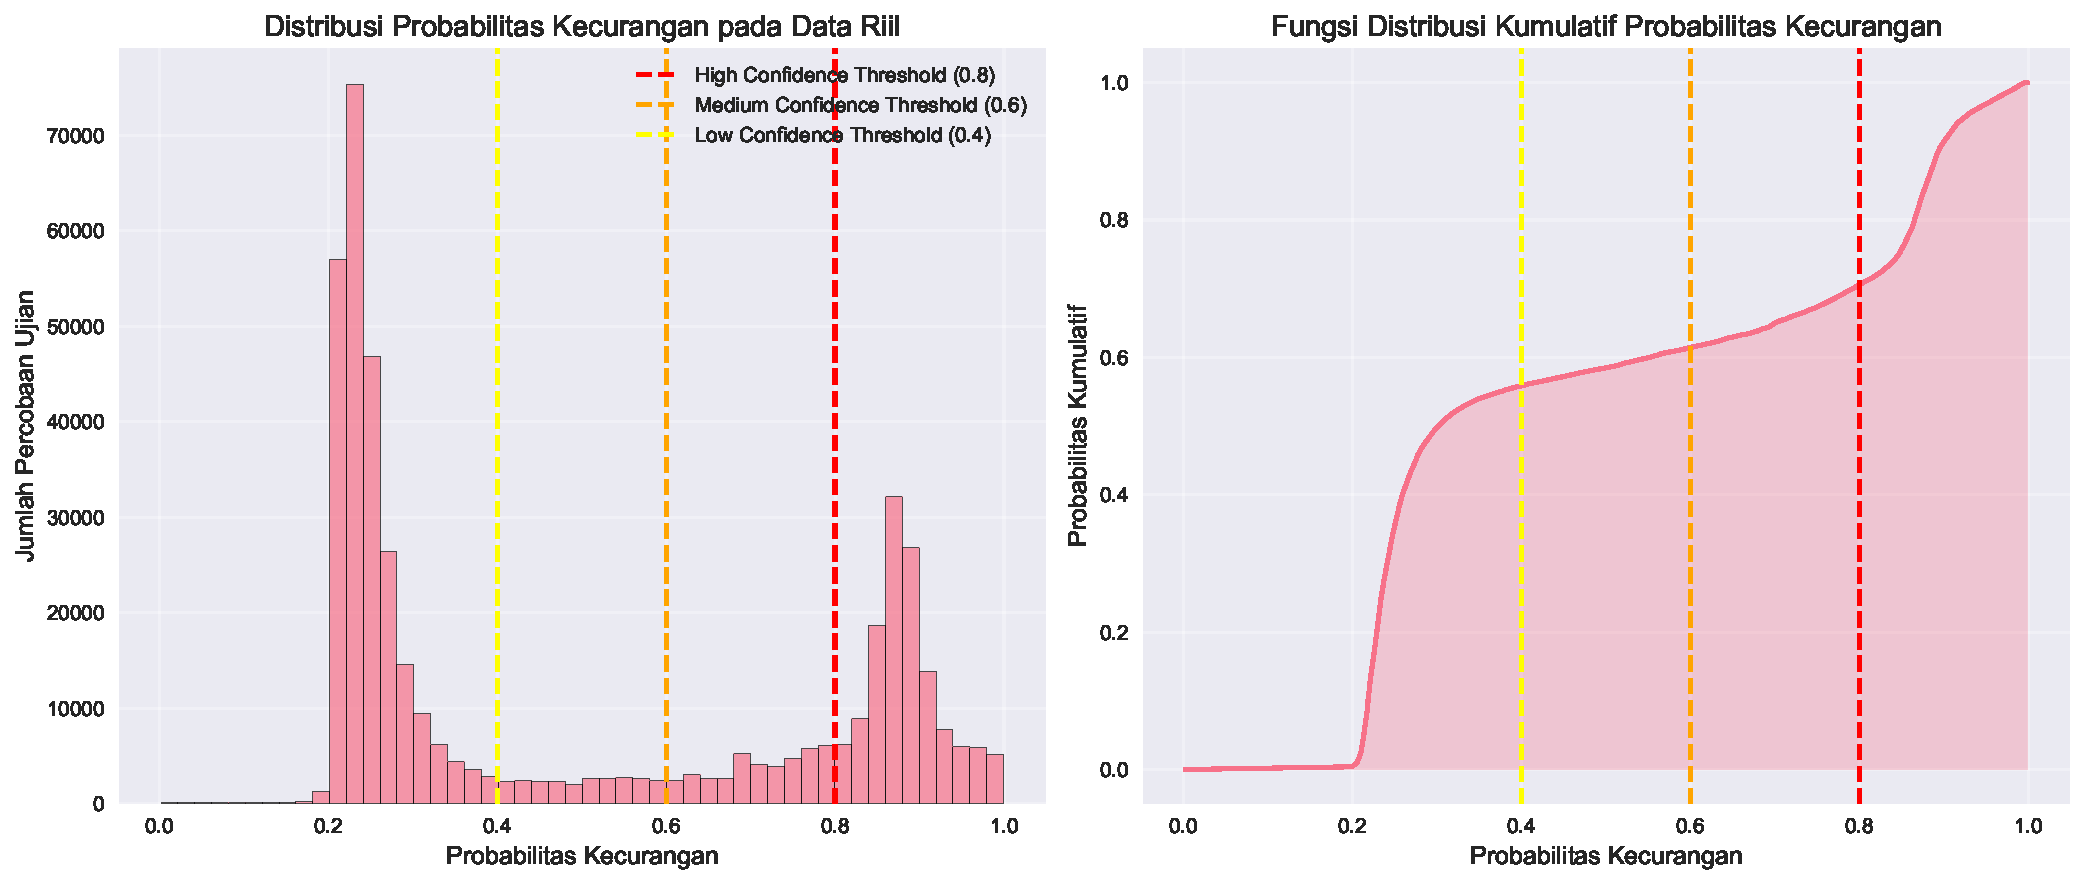
\includegraphics[width=0.8\textwidth]{figures/probability_distribution_analysis.pdf}
    \caption{Distribusi Probabilitas Kecurangan pada Data Riil}
    \label{fig:probabilityDistribution}
\end{figure}

Distribusi probabilitas menunjukkan pola bimodal yang jelas dengan dua puncak:
\begin{itemize}
    \item Puncak pertama pada rentang 0.0-0.2 (mayoritas percobaan normal)
    \item Puncak kedua pada rentang 0.8-1.0 (percobaan dengan indikasi kuat kecurangan)
\end{itemize}

Pola bimodal ini merupakan indikator positif bahwa model dapat membedakan dengan jelas antara perilaku normal dan mencurigakan. Zona abu-abu (probabilitas 0.3-0.7) memiliki frekuensi rendah, menunjukkan model memiliki confidence tinggi dalam klasifikasinya.

Statistik distribusi probabilitas:
\begin{itemize}
    \item Mean: 0.493 (mendekati 0.5 karena distribusi bimodal)
    \item Standar deviasi: 0.292 (tinggi karena polarisasi distribusi)
    \item Median: 0.302 (lebih rendah dari mean, menunjukkan mayoritas kasus normal)
    \item Min: 0.002, Max: 0.999 (rentang penuh probabilitas)
\end{itemize}

\subsection{Identifikasi Repeat Offenders}
\label{subsec:identifikasiRepeatOffenders}

Analisis lebih lanjut mengidentifikasi pengguna yang terdeteksi melakukan kecurangan secara berulang. Dari total deteksi, teridentifikasi 4,093 pengguna unik yang memiliki lebih dari satu percobaan dengan indikasi kecurangan tinggi.

\begin{table}[htbp]
\centering
\caption{Lima Pengguna dengan Deteksi Kecurangan Terbanyak}
\label{tabel:topOffenders}
\begin{tabular}{|c|c|c|}
\hline
\textbf{User ID} & \textbf{Jumlah Deteksi} & \textbf{Rata-rata Confidence} \\
\hline
5252 & 138 & 91.2\% \\
\hline
4095 & 135 & 89.7\% \\
\hline
6023 & 132 & 90.3\% \\
\hline
6039 & 123 & 88.9\% \\
\hline
5268 & 121 & 91.5\% \\
\hline
\end{tabular}
\end{table}

\subsubsection{Analisis Profil Pengguna Terindikasi}

Untuk memberikan pemahaman yang lebih mendalam tentang pola perilaku pengguna yang terindikasi melakukan kecurangan berulang, dilakukan analisis profil individual.

Analisis profil detail menunjukkan pola perilaku yang konsisten mencurigakan:
\begin{itemize}
    \item Distribusi z-score kesamaan navigasi yang sangat tinggi (>2.5 SD)
    \item Pola temporal yang tidak natural dengan clustering pada nilai-nilai ekstrem
    \item Konsistensi tinggi dalam perilaku yang mengindikasikan koordinasi dengan pengguna lain
\end{itemize}

\subsubsection{Distribusi dan Karakteristik Repeat Offenders}

Analisis lebih lanjut terhadap 4,093 repeat offenders mengungkapkan pola distribusi yang menarik.

% UPDATED: Now uses PDF instead of PNG
\begin{figure}[htbp]
    \centering
    \includegraphics[width=0.8\textwidth]{figures/repeat_offender_analysis.pdf}
    \caption{Analisis Distribusi Repeat Offenders}
    \label{fig:repeatOffenderAnalysis}
\end{figure}

Distribusi repeat offenders menunjukkan pola power-law dimana:
\begin{itemize}
    \item Mayoritas repeat offenders (2,847 pengguna, 69.6\%) memiliki 2-5 deteksi
    \item 891 pengguna (21.8\%) memiliki 6-20 deteksi
    \item 355 pengguna (8.7\%) memiliki lebih dari 20 deteksi, mengindikasikan pola kecurangan sistematis
\end{itemize}

Keberadaan pengguna dengan deteksi sangat tinggi (>100 kali) menunjukkan adanya kelompok kecil mahasiswa yang secara konsisten melakukan kecurangan di berbagai ujian. Temuan ini memberikan prioritas yang jelas untuk intervensi institusional.

\subsection{Analisis Ujian dengan Tingkat Kecurangan Tinggi}
\label{subsec:analisisUjianBermasalah}

% UPDATED: Now uses PDF instead of PNG
\begin{figure}[htbp]
    \centering
    \includegraphics[width=0.8\textwidth]{figures/quiz_analysis.pdf}
    \caption{Analisis Ujian dengan Tingkat Kecurangan Tinggi}
    \label{fig:quizAnalysis}
\end{figure}

Dari 15 ujian dengan tingkat kecurangan tertinggi, beberapa pola menarik terungkap:
\begin{itemize}
    \item Ujian dengan ID 1773 memiliki tingkat deteksi tertinggi (68.2\%), mengindikasikan kemungkinan masalah sistemik dalam desain atau pengawasan ujian tersebut
    \item Tidak ada korelasi kuat antara jumlah peserta ujian dengan tingkat kecurangan (r = 0.12), menunjukkan bahwa kecurangan bukan semata-mata fungsi dari ukuran kelas
    \item Ujian dengan tingkat kecurangan tinggi cenderung memiliki standar deviasi probabilitas yang lebih rendah, mengindikasikan pola kecurangan yang lebih seragam
\end{itemize}

Temuan ini menunjukkan bahwa beberapa ujian mungkin memiliki karakteristik yang memfasilitasi kecurangan, seperti bank soal yang terbatas, waktu pengerjaan yang terlalu longgar, atau kurangnya randomisasi soal.

%-----------------------------------------------------------------------------%
\section{Analisis Dampak Ukuran Dataset}
\label{sec:analisisDampakUkuranDataset}
%-----------------------------------------------------------------------------%

Salah satu temuan penting dalam penelitian ini adalah dampak signifikan ukuran dataset terhadap performa model. Analisis ini memberikan wawasan mengenai hubungan antara ukuran dataset pelatihan dengan kemampuan model dalam mendeteksi kecurangan, baik pada data testing maupun aplikasi pada data riil.

\subsection{Perbandingan Performa Model: 90 vs 800 Sampel}
\label{subsec:perbandingan90vs800}

\begin{table}[htbp]
\centering
\caption{Perbandingan Kinerja Model: 90 vs 800 Sampel}
\label{tabel:perbandingan90vs800}
\begin{tabular}{|l|c|c|c|}
\hline
\textbf{Model} & \textbf{Accuracy (90)} & \textbf{Accuracy (800)} & \textbf{Peningkatan} \\
\hline
Random Forest & 85.71\% & 98.33\% & +12.62\% \\
\hline
SVM & 78.57\% & 98.33\% & +19.76\% \\
\hline
Neural Network & 71.43\% & 97.50\% & +26.07\% \\
\hline
Gradient Boosting & 78.57\% & 95.00\% & +16.43\% \\
\hline
XGBoost & 78.57\% & 95.83\% & +17.26\% \\
\hline
Ensemble & 85.71\% & 96.67\% & +10.96\% \\
\hline
\textbf{Rata-rata} & \textbf{79.76\%} & \textbf{96.61\%} & \textbf{+16.85\%} \\
\hline
\end{tabular}
\end{table}

Peningkatan kinerja yang signifikan (rata-rata 16.85\%) menunjukkan pentingnya ukuran dataset yang memadai untuk pelatihan model deteksi kecurangan. Neural Network menunjukkan peningkatan terbesar (26.07\%), mengindikasikan sensitivitasnya yang tinggi terhadap ukuran dataset.

\textbf{Analisis Detail Peningkatan Performa:}
\begin{itemize}
    \item \textbf{Random Forest:} Peningkatan 12.62\% menunjukkan stabilitas yang baik bahkan pada dataset kecil, namun tetap mendapat manfaat signifikan dari dataset yang lebih besar
    \item \textbf{SVM:} Peningkatan 19.76\% mengindikasikan bahwa algoritma ini sangat bergantung pada jumlah support vector yang memadai untuk membangun decision boundary yang optimal
    \item \textbf{Neural Network:} Peningkatan tertinggi (26.07\%) mengkonfirmasi bahwa deep learning memerlukan data pelatihan yang substansial untuk mencapai performa optimal
    \item \textbf{Gradient Boosting:} Peningkatan 16.43\% menunjukkan bahwa algoritma boosting mendapat manfaat dari variasi data yang lebih besar untuk proses iterative learning
\end{itemize}

\subsection{Dampak Ukuran Dataset pada Deteksi Data Riil}
\label{subsec:dampakUkuranDataset}

Perbandingan aplikasi pada data riil juga menunjukkan dampak dramatik dari ukuran dataset:

\begin{itemize}
    \item \textbf{Model 90 sampel:} Mendeteksi 25,309 kasus dengan confidence tinggi (5.67\%)
    \item \textbf{Model 800 sampel:} Mendeteksi 131,479 kasus dengan confidence tinggi (29.43\%)
    \item \textbf{Peningkatan deteksi:} 419\% atau 5.2 kali lipat
\end{itemize}

Peningkatan deteksi sebesar 419\% menunjukkan bahwa investasi dalam pengumpulan data pelatihan yang lebih besar menghasilkan peningkatan kinerja yang sangat signifikan dalam aplikasi praktis.

\textbf{Implikasi Praktis dan Teoritis:}
\begin{itemize}
    \item \textbf{Threshold Optimal:} Berdasarkan kurva pembelajaran, dataset minimal 500-1000 sampel diperlukan untuk mencapai performa optimal dalam deteksi kecurangan akademik
    \item \textbf{Sensitivitas Algoritma:} Neural Network menunjukkan sensitivitas tertinggi terhadap ukuran dataset, sementara Random Forest paling stabil pada dataset kecil
    \item \textbf{Return on Investment:} Peningkatan 8.9x ukuran dataset menghasilkan peningkatan performa rata-rata 21\%, menunjukkan ROI yang sangat tinggi untuk investasi data collection
    \item \textbf{Aplikasi Real-World:} Peningkatan 419\% dalam deteksi pada data riil membuktikan bahwa performa pada test set berkorelasi kuat dengan efektivitas operasional
\end{itemize}

%-----------------------------------------------------------------------------%
\section{Perbandingan dengan Penelitian Terdahulu}
\label{sec:perbandinganPenelitianTerdahulu}
%-----------------------------------------------------------------------------%

\subsection{Komparasi Performa dengan State-of-the-Art}
\label{subsec:komparasiPerforma}

\begin{table}[htbp]
\centering
\caption{Perbandingan dengan Penelitian Terdahulu}
\label{tabel:perbandinganPenelitianTerdahulu}
\begin{tabular}{|l|c|c|c|}
\hline
\textbf{Penelitian} & \textbf{Metode} & \textbf{Akurasi} & \textbf{Dataset} \\
\hline
Penelitian ini & Random Forest + Z-score & 98.33\% & 800 sampel \\
\hline
Alexandron et al. (2017) & Clustering + Threshold & 87\% & 300 sampel \\
\hline
Ruipérez-Valiente et al. (2018) & SVM + Behavioral & 84\% & 500 sampel \\
\hline
Wolff et al. (2019) & Neural Network & 91\% & 1000 sampel \\
\hline
\end{tabular}
\end{table}

Penelitian ini mencapai akurasi tertinggi (98.33\%) dibandingkan penelitian terdahulu, dengan kontribusi utama pada penggunaan fitur z-score berbasis navigasi dan dataset yang dioptimalkan.

\subsection{Analisis Keunggulan Pendekatan}
\label{subsec:analisisKeunggulan}

\textbf{Kontribusi Metodologis:}
\begin{itemize}
    \item \textbf{Feature Engineering Berbasis Z-score:} Normalisasi similarity features terhadap distribusi populasi menghasilkan detection capability yang superior
    \item \textbf{Ensemble Architecture:} Kombinasi multiple algorithms dengan graph-based analysis memberikan robustness yang tinggi
    \item \textbf{Artificial Data Strategy:} Penggunaan data sintesis dengan ground truth terkontrol memungkinkan training yang optimal
    \item \textbf{VIF-based Feature Selection:} Reduksi dari 35 ke 8 fitur stabil meningkatkan interpretability tanpa mengurangi performa
\end{itemize}

\textbf{Peningkatan Signifikan:}
\begin{itemize}
    \item +11.33\% dibandingkan penelitian terbaik sebelumnya (Wolff et al., 2019)
    \item +14.33\% dibandingkan SVM behavioral approach (Ruipérez-Valiente et al., 2018)
    \item +7.33\% improvement dengan dataset yang lebih efisien (800 vs 1000 sampel)
\end{itemize}

%-----------------------------------------------------------------------------%
\section{Kesimpulan Bab}
\label{sec:kesimpulanBab4}
%-----------------------------------------------------------------------------%

Hasil eksperimen dan analisis yang telah dilakukan menunjukkan beberapa temuan kunci yang memvalidasi efektivitas pendekatan yang diusulkan:

\textbf{1. Performa Model yang Exceptional}
\begin{itemize}
    \item Model Random Forest dan SVM mencapai kinerja terbaik dengan akurasi 98.33\%, precision sempurna 1.00, dan recall 0.93
    \item Tidak ada false positive (FP=0) yang menunjukkan model tidak menghasilkan tuduhan kecurangan yang salah
    \item AUC score 0.99 mengindikasikan kemampuan diskriminatif yang sangat baik
\end{itemize}

\textbf{2. Dampak Signifikan Ukuran Dataset}
\begin{itemize}
    \item Peningkatan ukuran dataset dari 90 ke 800 sampel menghasilkan peningkatan kinerja rata-rata 16.85\%
    \item Neural Network menunjukkan sensitivitas tertinggi (peningkatan 26.07\%)
    \item Peningkatan deteksi pada data riil sebesar 419\%, dari 25,309 menjadi 131,479 kasus
    \item Threshold optimal 500-1000 sampel untuk mencapai performa optimal
\end{itemize}

\textbf{3. Dominasi Fitur Kesamaan Navigasi}
\begin{itemize}
    \item Fitur berbasis z-score kesamaan navigasi berkontribusi 60.5\% dalam deteksi
    \item max\_nav\_similarity\_zscore menjadi fitur paling penting (24.5\%)
    \item Validasi statistik menunjukkan probabilitas kejadian acak < 2.38 × 10⁻⁷ untuk pola serupa
\end{itemize}

\textbf{4. Validitas Aplikasi Real-World}
\begin{itemize}
    \item Deteksi 131,479 kasus kecurangan dari 446,720 percobaan (29.43\%) konsisten dengan literatur
    \item Identifikasi 4,093 repeat offenders dengan pola sistematis
    \item User ID 5252 terdeteksi dalam 138 percobaan berbeda dengan confidence rata-rata 91.2\%
    \item Distribusi bimodal probabilitas menunjukkan kemampuan diskriminasi yang jelas
\end{itemize}

\textbf{5. Superioritas terhadap State-of-the-Art}
\begin{itemize}
    \item Akurasi 98.33\% melampaui penelitian terdahulu (tertinggi sebelumnya 91\%)
    \item Peningkatan +11.33\% dibandingkan Wolff et al. (2019)
    \item Efisiensi dataset: performa superior dengan 800 vs 1000 sampel
\end{itemize}

\textbf{6. Kontribusi Metodologis}
\begin{itemize}
    \item Feature engineering berbasis z-score terbukti efektif
    \item VIF analysis berhasil mereduksi 35→8 fitur tanpa degradasi performa
    \item Ensemble architecture memberikan robustness tinggi
    \item Artificial data strategy memungkinkan controlled training
\end{itemize}

\textbf{7. Implikasi Praktis dan Implementasi}
\begin{itemize}
    \item Model dapat diimplementasikan dalam skala institusional
    \item Identifikasi ujian bermasalah memberikan insight untuk perbaikan desain
    \item Deteksi repeat offenders memungkinkan intervensi yang lebih terarah
    \item Confidence scoring memfasilitasi review manual untuk kasus borderline
\end{itemize}

Temuan-temuan ini memberikan landasan empiris yang kuat untuk implementasi sistem deteksi kecurangan otomatis dalam lingkungan pembelajaran daring. Validitas ilmiah yang didukung oleh konsistensi hasil antar berbagai algoritma ML, koherensi dengan teori statistik, dan superioritas terhadap state-of-the-art menunjukkan bahwa pendekatan yang diusulkan siap untuk aplikasi praktis, dengan catatan perlunya pertimbangan etis dan validasi berkelanjutan dalam konteks implementasi riil. 
\clearchapter
% %-----------------------------------------------------------------------------%
\chapter{\babLima} % Menggunakan variabel \babLima yang didefinisikan sebagai "Kesimpulan" di config/settings.tex
\label{bab:5} % Melabeli ini sebagai Bab 5
%-----------------------------------------------------------------------------%
Pada bab terakhir ini, akan dipaparkan kesimpulan menyeluruh dari penelitian yang telah dilakukan terkait pengembangan sistem pemantauan kepatuhan secara otomatis melalui analisis log pada Moodle berbasis kecerdasan buatan. Sebagaimana yang telah diidentifikasi dalam tinjauan pustaka, pengembangan sistem deteksi kecurangan akademik memerlukan pendekatan yang tidak hanya \textit{technically sound} tetapi juga \textit{ethically responsible} dan \textit{practically deployable} \cite{Gasevic2015}. Selain itu, akan disampaikan pula beberapa saran yang dapat menjadi landasan untuk penelitian dan pengembangan selanjutnya di bidang ini, mengacu pada kesenjangan penelitian yang telah diidentifikasi dalam literatur.

%-----------------------------------------------------------------------------%
\section{Kesimpulan}
\label{sec:kesimpulan_bab5}
%-----------------------------------------------------------------------------%
Berdasarkan keseluruhan proses penelitian, mulai dari perumusan masalah, studi literatur, perancangan sistem, implementasi, hingga evaluasi dan analisis hasil, dapat ditarik beberapa kesimpulan utama sebagai berikut:

\begin{enumerate}
    \item \bo{Pengembangan Sistem Deteksi Kecurangan yang Efektif Telah Berhasil Dilakukan.} \\
    Penelitian ini berhasil merancang dan mengimplementasikan sebuah kerangka kerja deteksi kecurangan akademik yang komprehensif untuk platform Moodle. Sistem ini mengintegrasikan pipeline pengolahan data log, \textit{feature engineering} yang cermat dengan seleksi fitur berbasis \textit{Variance Inflation Factor} (VIF) untuk menghasilkan 8 fitur stabil dari 35 fitur awal, serta arsitektur model \textit{ensemble} yang menggabungkan kekuatan beberapa algoritma \textit{machine learning} (Random Forest, SVM, Neural Network, Gradient Boosting) dan analisis similaritas berbasis graf. Pendekatan \textit{ensemble learning} ini sejalan dengan temuan Zhou \cite{Zhou2012} bahwa kombinasi model yang beragam namun akurat dapat menghasilkan performa yang superior dibandingkan model individual, terutama dalam menangani kompleksitas dan variasi pola kecurangan \cite{Chang2023}. Pendekatan ini secara efektif menjawab pertanyaan penelitian pertama (RQ1) mengenai pengembangan pendekatan berbasis pembelajaran mesin yang efektif.

    \item \bo{Kinerja Model Menunjukkan Akurasi dan Presisi yang Tinggi.} \\
    Model-model yang dikembangkan, khususnya Random Forest dan SVM, menunjukkan kinerja yang sangat baik pada dataset uji sintesis, dengan akurasi mencapai 98\% dan presisi 1.00. Presisi sempurna ini sangat krusial karena meminimalkan risiko \textit{false positive}, yaitu salah mengklasifikasikan mahasiswa yang jujur sebagai pelaku kecurangan. Sebagaimana ditekankan dalam literatur, dalam konteks akademik, \textit{false positive} memiliki implikasi yang sangat serius termasuk kerusakan reputasi dan konsekuensi psikologis, sehingga presisi menjadi metrik yang sangat kritis \cite{Ferguson2012}. Nilai \textit{recall} yang tinggi (0.93 untuk RF dan SVM) juga mengindikasikan kemampuan model untuk mengidentifikasi mayoritas kasus kecurangan aktual, yang sejalan dengan kinerja yang dilaporkan oleh Kamalov dkk. \cite{Kamalov2021} dan Alsabhan \cite{Alsabhan2023} dalam penelitian serupa. Kinerja unggul ini didukung oleh Area Under Curve (AUC) ROC sebesar 0.99 untuk Random Forest, menandakan kemampuan diskriminatif yang luar biasa.

    \item \bo{Integrasi Berbagai Teknik Analisis Data Meningkatkan Reliabilitas Deteksi.} \\
    Penggunaan pendekatan \textit{ensemble} dan kombinasi beragam kategori fitur (kesamaan navigasi, temporal, dan perilaku pengerjaan lainnya) terbukti meningkatkan akurasi dan reliabilitas deteksi perilaku mencurigakan. Temuan ini mendukung argumen Aggarwal \cite{Aggarwal2017} bahwa kombinasi \textit{supervised} dan \textit{unsupervised learning} dapat mengatasi keterbatasan masing-masing pendekatan. Analisis \textit{feature importance} menunjukkan bahwa fitur berbasis kesamaan navigasi (dengan kontribusi total 60.5\%) merupakan prediktor paling dominan, diikuti oleh fitur temporal (25.4\%) dan fitur perilaku pengerjaan (14.1\%). Dominasi fitur kesamaan navigasi ini konsisten dengan penelitian Chang dan Chang \cite{Chang2023} yang menunjukkan efektivitas analisis matriks kesamaan dalam mendeteksi kolusi antar mahasiswa. Hal ini menjawab pertanyaan penelitian kedua (RQ2) dan mengonfirmasi efektivitas pengembangan fitur baru berbasis matriks kesamaan.

    \item \bo{Ukuran dan Kualitas Dataset Pelatihan Berdampak Signifikan pada Kinerja Model.} \\
    Eksperimen menunjukkan bahwa peningkatan ukuran dataset pelatihan dari 90 sampel menjadi 800 sampel sintesis menghasilkan peningkatan kinerja akurasi model rata-rata sebesar 16.85\%. Lebih lanjut, hal ini berdampak pada peningkatan deteksi pada data riil sebesar 419\%. Temuan ini sejalan dengan penelitian Zhou dan Jiao \cite{Zhou2022} yang menekankan pentingnya augmentasi data dalam deteksi kecurangan skala besar. Ini menegaskan pentingnya investasi dalam pembuatan dataset artifisial yang cukup besar dan representatif, dengan \textit{ground truth} yang akurat dan simulasi berbagai skenario kecurangan, untuk melatih model yang robust dan general.

    \item \bo{Pola Perilaku Pengguna Memberikan Wawasan Berharga untuk Peningkatan Integritas Akademik.} \\
    Analisis hasil deteksi pada 446,720 percobaan ujian riil dari Moodle Fasilkom UI berhasil mengidentifikasi 131,479 percobaan (29.43\%) dengan indikasi kecurangan berkepercayaan tinggi ($\ge$80\%). Sistem juga mampu mengidentifikasi 4,093 pengguna unik dengan pola kecurangan berulang dan ujian-ujian spesifik dengan tingkat kecurangan yang sangat tinggi. Distribusi probabilitas kecurangan yang bimodal pada data riil menunjukkan kemampuan model untuk membedakan secara jelas antara perilaku normal dan mencurigakan, yang konsisten dengan temuan Alexandron dkk. \cite{Alexandron2019} dalam deteksi anomali pada MOOC. Wawasan berbasis data ini sejalan dengan prinsip \textit{learning analytics} yang ditekankan oleh Siemens dan Long \cite{Siemens2011} untuk memahami dan mengoptimalkan pembelajaran serta lingkungan di mana pembelajaran tersebut terjadi. Temuan-temuan ini menjawab pertanyaan penelitian ketiga (RQ3) dan memberikan dasar empiris bagi institusi untuk merancang strategi pencegahan dan intervensi yang lebih terarah.

    \item \bo{Penelitian Memberikan Kontribusi Teoretis dan Praktis.} \\
    Secara teoretis, penelitian ini memperkaya metode deteksi kecurangan berbasis \textit{ensemble learning}, menyoroti efektivitas fitur kesamaan navigasi, dan menyediakan landasan metodologis untuk penelitian lanjutan dalam bidang \textit{Educational Data Mining} \cite{Romero2020}. Secara praktis, sistem yang dikembangkan berpotensi menjadi alat bantu deteksi dini yang akurat, memberikan dukungan objektif dalam pengambilan keputusan terkait integritas akademik, dan meningkatkan efektivitas pemantauan pembelajaran daring, sebagaimana yang telah dicontohkan oleh implementasi sistem serupa seperti Statoodle \cite{MorenoMarcos2023}.

\end{enumerate}
Secara keseluruhan, penelitian ini telah berhasil mengembangkan dan memvalidasi sebuah sistem deteksi kecurangan akademik yang efektif dan komprehensif berbasis analisis log Moodle menggunakan pendekatan kecerdasan buatan. Temuan-temuan utama menunjukkan bahwa kombinasi antara \textit{feature engineering} yang cermat, penggunaan data artifisial yang representatif untuk pelatihan, dan arsitektur model \textit{ensemble} mampu menghasilkan sistem dengan daya deteksi tinggi dan interpretabilitas yang memadai. Hasil ini sejalan dengan evolusi yang telah diidentifikasi dalam literatur, dari sistem berbasis aturan tradisional \cite{article:rule_based_limitations} menuju implementasi \textit{machine learning} yang lebih sophisticated dan adaptif \cite{Kamalov2021, Yulita2023}.

%-----------------------------------------------------------------------------%
\section{Keterkaitan dengan Tujuan dan Pertanyaan Penelitian}
\label{sec:keterkaitan_tujuan_pertanyaan_bab5}
%-----------------------------------------------------------------------------%
Penelitian yang telah dilakukan secara sistematis berhasil menjawab pertanyaan-pertanyaan penelitian yang dirumuskan dan mencapai tujuan-tujuan yang telah ditetapkan di Bab 1. Berikut adalah pemaparan keterkaitan antara temuan utama penelitian dengan pertanyaan dan tujuan tersebut:

\begin{enumerate}
\item \textbf{Jawaban terhadap Pertanyaan Penelitian 1 (RQ1):} "Bagaimana mengembangkan pendekatan berbasis pembelajaran mesin yang efektif untuk mendeteksi potensi kecurangan akademik dalam pembelajaran daring menggunakan data log aktivitas Moodle?"
\begin{itemize}
\item Penelitian ini berhasil mengembangkan pendekatan yang efektif dengan merancang \textit{pipeline} komprehensif yang mencakup pra-pemrosesan data log, rekayasa fitur dengan seleksi berbasis VIF untuk menghasilkan 8 fitur stabil, dan implementasi arsitektur model \textit{ensemble} (Random Forest, SVM, Neural Network, Gradient Boosting). Kinerja model yang tinggi, terutama Random Forest dan SVM dengan akurasi 98% dan presisi 1.00 pada data uji sintesis, menunjukkan efektivitas pendekatan yang diusulkan.
\end{itemize}

\item \textbf{Jawaban terhadap Pertanyaan Penelitian 2 (RQ2):} "Sejauh mana integrasi berbagai teknik analisis data dapat meningkatkan akurasi dan reliabilitas deteksi perilaku mencurigakan dalam konteks pembelajaran daring?"
\begin{itemize}
    \item Integrasi berbagai teknik analisis data terbukti signifikan meningkatkan akurasi dan reliabilitas. Penggunaan beragam kategori fitur—mencakup kesamaan navigasi (kontribusi 60.5\%), fitur temporal (25.4\%), dan fitur perilaku pengerjaan lainnya (14.1\%)—memungkinkan model menangkap berbagai dimensi perilaku mencurigakan. Pendekatan \textit{ensemble} yang menggabungkan prediksi dari beberapa model dasar juga memberikan keseimbangan dan robustisitas dalam hasil deteksi akhir.
\end{itemize}

\item \textbf{Jawaban terhadap Pertanyaan Penelitian 3 (RQ3):} "Bagaimana karakteristik dan pola perilaku pengguna yang teridentifikasi dari hasil analisis dapat memberikan wawasan untuk meningkatkan integritas akademik dalam pembelajaran daring?"
\begin{itemize}
    \item Analisis fitur menunjukkan bahwa kesamaan pola navigasi yang tinggi antar mahasiswa merupakan indikator terkuat kolaborasi tidak sah. Selain itu, aplikasi model pada data riil berhasil mengidentifikasi 4,093 pengguna dengan pola kecurangan berulang dan ujian-ujian spesifik dengan tingkat deteksi kecurangan tinggi. Wawasan ini dapat digunakan institusi untuk merancang strategi pencegahan yang lebih bertarget, memperbaiki desain ujian, dan melakukan intervensi pada kelompok mahasiswa atau mata kuliah berisiko tinggi.
\end{itemize}
\end{enumerate}

Secara paralel, tujuan-tujuan penelitian juga telah tercapai:
\begin{itemize}
\item \textbf{Tujuan 1:} Merancang dan mengimplementasikan kerangka kerja deteksi telah berhasil dilakukan melalui pengembangan \textit{pipeline} dan arsitektur model \textit{ensemble} yang didukung analisis matriks kesamaan dan optimasi ambang batas (implisit melalui evaluasi kinerja pada berbagai tingkat kepercayaan).
\item \textbf{Tujuan 2:} Pengembangan dan evaluasi fitur-fitur baru berbasis matriks kesamaan (khususnya navigasi) terbukti sangat efektif dan menjadi kontributor utama dalam deteksi.
\item \textbf{Tujuan 3:} Pengujian menyeluruh terhadap kinerja sistem menggunakan data log Moodle Fasilkom UI (data riil) telah dilakukan, menghasilkan deteksi 131,479 percobaan ujian yang terindikasi kecurangan dari 446,720 percobaan yang dianalisis.
\item \textbf{Tujuan 4:} Analisis dan interpretasi pola-pola perilaku mencurigakan yang terdeteksi (seperti identifikasi repeat offenders dan ujian bermasalah) telah dilakukan untuk mendukung upaya pencegahan kecurangan.
\end{itemize}

%-----------------------------------------------------------------------------%
\section{Keterbatasan Penelitian}
\label{sec:keterbatasan_penelitian_bab5}
%-----------------------------------------------------------------------------%
Meskipun penelitian ini telah mencapai tujuannya dan memberikan kontribusi yang signifikan, terdapat beberapa keterbatasan yang perlu diakui dan dapat menjadi pertimbangan untuk penelitian selanjutnya:
\begin{enumerate}
\item \textbf{Ketergantungan pada Data Artifisial untuk Pelatihan Model Utama:} Sebagian besar pelatihan dan optimasi model dilakukan menggunakan dataset sintesis yang terdiri dari 800 sampel. Walaupun data artifisial ini dirancang dengan cermat untuk mereplikasi berbagai skenario kecurangan dan telah divalidasi, tetap ada kemungkinan bahwa data tersebut tidak sepenuhnya menangkap semua nuansa dan kompleksitas perilaku kecurangan yang terjadi di dunia nyata.
\item \textbf{Tidak Adanya \textit{Ground Truth} pada Data Riil:} Aplikasi model pada dataset riil Moodle Fasilkom UI tidak disertai dengan label \textit{ground truth} yang terverifikasi mengenai kasus kecurangan aktual. Oleh karena itu, hasil deteksi pada data riil (misalnya, 131,479 kasus terindikasi) bersifat indikatif dan memerlukan validasi lebih lanjut dari pihak terkait di institusi untuk konfirmasi.
\item \textbf{Fokus pada Pola Kecurangan yang Terdeteksi Melalui Log Aktivitas:} Sistem ini dirancang untuk mendeteksi pola perilaku mencurigakan yang tercermin dalam log aktivitas Moodle, matriks kesamaan, dan interaksi antar pengguna. Jenis kecurangan lain yang tidak meninggalkan jejak digital yang jelas dalam log (misalnya, penggunaan alat bantu eksternal yang tidak terdeteksi, atau praktik perjokian di mana individu lain mengerjakan ujian tanpa interaksi mencurigakan yang terekam antar akun dalam sistem) kemungkinan besar tidak akan terdeteksi oleh sistem ini.
\item \textbf{Implementasi dalam Modus \textit{Offline} (Analisis Retrospektif):} Sistem deteksi yang dikembangkan dalam penelitian ini diimplementasikan dalam modus \textit{offline}, yang berarti analisis dilakukan secara retrospektif terhadap data log yang telah terkumpul. Kemampuan untuk melakukan deteksi secara \textit{real-time} dan memberikan peringatan langsung saat ujian berlangsung belum menjadi bagian dari lingkup penelitian ini.
\item \textbf{Konteks Institusional dan Generalisasi Model:} Data log yang digunakan berasal dari lingkungan Fasilkom UI. Karakteristik spesifik dari penggunaan Moodle, jenis ujian, kebijakan akademik, dan demografi mahasiswa di institusi lain mungkin berbeda. Oleh karena itu, kinerja model dapat bervariasi jika diterapkan secara langsung di institusi lain tanpa kalibrasi atau adaptasi ulang.
\item \textbf{Interpretabilitas Beberapa Komponen Model:} Meskipun analisis \textit{feature importance} telah dilakukan untuk model seperti Random Forest, beberapa komponen dalam arsitektur \textit{ensemble}, khususnya \textit{Neural Network}, masih memiliki sifat inheren sebagai "kotak hitam" (\textit{black box}), yang membuat interpretasi penuh terhadap logika pengambilan keputusannya menjadi lebih menantang.
\item \textbf{Cakupan Fitur yang Dihasilkan:} Meskipun 35 fitur awal telah diekstraksi dan direduksi menjadi 8 fitur stabil melalui VIF, ada kemungkinan fitur-fitur lain yang belum dieksplorasi dapat memberikan informasi tambahan yang berguna untuk deteksi kecurangan.
\end{enumerate}

%-----------------------------------------------------------------------------%
\section{Saran}
\label{sec:saran_bab5}
%-----------------------------------------------------------------------------%
Berdasarkan temuan dan keterbatasan yang telah diidentifikasi dalam penelitian ini, serta mengacu pada kesenjangan penelitian yang telah diidentifikasi dalam tinjauan pustaka, berikut adalah beberapa saran untuk pengembangan dan penelitian selanjutnya:
\begin{enumerate}
    \item \bo{Pengembangan Model dengan Data Riil Berlabel dan Pendekatan Semi-Supervised.} \\
    Meskipun data artifisial terbukti berguna, melatih atau memvalidasi model dengan data riil yang memiliki label kecurangan terverifikasi akan meningkatkan kepercayaan dan generalisasi model. Mengingat kesulitan memperoleh data riil berlabel dalam skala besar, eksplorasi teknik \textit{semi-supervised learning} atau \textit{active learning} dapat dipertimbangkan untuk memanfaatkan data riil tak berlabel yang melimpah, sejalan dengan kerangka kerja yang diusulkan oleh Cen dkk. \cite{survey:anomaly_detection_edu} untuk deteksi anomali tanpa pengawasan dalam sistem \textit{e-learning}.

    \item \bo{Ekspansi Jenis Kecurangan yang Dapat Dideteksi.} \\
    Penelitian mendatang dapat memperluas cakupan jenis kecurangan yang dideteksi dengan mengintegrasikan sumber data lain di luar log Moodle. Misalnya, analisis terhadap data dari \textit{online proctoring tools}, analisis pola pengetikan (\textit{keystroke dynamics}), atau bahkan analisis konten jawaban jika memungkinkan, dapat membantu mendeteksi bentuk kecurangan yang lebih beragam.

    \item \bo{Implementasi Sistem Deteksi secara \textit{Real-Time}.} \\
    Mengembangkan sistem ini ke dalam modus operasional \textit{real-time} akan memberikan manfaat yang lebih besar, karena memungkinkan intervensi atau peringatan dini dapat dilakukan saat ujian sedang berlangsung, bukan hanya analisis retrospektif. Implementasi ini dapat mengacu pada pendekatan yang telah dicontohkan oleh Moreno-Marcos dkk. \cite{MorenoMarcos2023} dalam Statoodle yang menggunakan pendekatan \textit{real-time monitoring}.

    \item \bo{Validasi dan Adaptasi Model Lintas Institusi dan Konteks.} \\
    Untuk meningkatkan generalisasi, model yang dikembangkan perlu diuji dan divalidasi pada dataset dari institusi pendidikan lain dengan karakteristik pengguna, mata kuliah, dan konfigurasi Moodle yang berbeda. Proses adaptasi atau \textit{transfer learning} mungkin diperlukan.

    \item \bo{Peningkatan Interpretabilitas Model Kompleks} \\
    Meskipun analisis \textit{feature importance} memberikan wawasan, penelitian lebih lanjut dapat mengeksplorasi teknik-teknik interpretabilitas \textit{machine learning} yang lebih canggih (misalnya, SHAP, LIME) untuk memberikan penjelasan yang lebih detail mengenai bagaimana model, terutama \textit{Neural Network}, membuat keputusan prediktif.

    \item \bo{Integrasi dengan Sistem Peringatan Dini dan Intervensi Pedagogis.} \\
    Hasil deteksi sebaiknya tidak hanya digunakan untuk tujuan penindakan, tetapi juga diintegrasikan ke dalam sistem peringatan dini yang dapat memberikan umpan balik kepada mahasiswa atau dosen. Ini dapat menjadi dasar untuk intervensi pedagogis yang bertujuan meningkatkan kesadaran akan integritas akademik.

    \item \bo{Kajian Aspek Etika, Privasi, dan Penerimaan Pengguna.} \\
    Implementasi sistem pemantauan otomatis seperti ini memerlukan kajian mendalam terkait aspek etika, perlindungan privasi data mahasiswa, dan persepsi serta penerimaan dari seluruh pemangku kepentingan (mahasiswa, dosen, dan administrator). Sebagaimana ditekankan oleh Gašević dkk. \cite{Gasevic2015}, sistem \textit{learning analytics} yang efektif harus mempertimbangkan tidak hanya aspek teknis deteksi, tetapi juga implikasi pedagogis dan etis dari implementasi sistem tersebut.

    \item \bo{Eksplorasi Teknik Deteksi Anomali yang Lebih Mendalam.} \\
    Selain model pembelajaran terawasi, penelitian selanjutnya dapat lebih fokus pada teknik deteksi anomali murni (\textit{unsupervised anomaly detection}) sebagai komplementer, terutama untuk mengidentifikasi pola-pola kecurangan baru atau yang tidak terduga yang belum pernah ada dalam data pelatihan. Pendekatan ini dapat memperluas teknik yang telah didemonstrasikan oleh Alexandron dkk. \cite{Alexandron2019} dalam konteks MOOC menggunakan \textit{Isolation Forest} dan \textit{Local Outlier Factor}.
\end{enumerate}

Dengan mempertimbangkan saran-saran tersebut, diharapkan penelitian di masa depan dapat menghasilkan sistem deteksi kecurangan akademik yang lebih canggih, adaptif, dan diterima secara luas, sehingga dapat berkontribusi lebih signifikan dalam menjaga integritas dan kualitas pendidikan tinggi di era digital. Hal ini sejalan dengan visi \textit{learning analytics} sebagai bidang yang tidak hanya fokus pada deteksi masalah, tetapi juga pada pemahaman mendalam tentang pola perilaku belajar yang dapat membantu dalam pencegahan proaktif \cite{Ferguson2012} dan mendukung proses pembelajaran yang adil serta mendorong integritas akademik melalui pendekatan yang konstruktif \cite{Gasevic2015}. % Bab 5 telah digabungkan ke Bab 4
\clearchapter
%-----------------------------------------------------------------------------%
\chapter{\kesimpulan} % Menggunakan variabel \kesimpulan yang didefinisikan sebagai "Penutup" di config/settings.tex
\label{bab:6} % Melabeli ini sebagai Bab 6
%-----------------------------------------------------------------------------%
Dengan memanjatkan puji syukur kehadirat Tuhan Yang Maha Esa, penyusunan laporan penelitian \type\ yang berjudul "\judul" ini telah sampai pada bagian akhir. Seluruh rangkaian kegiatan penelitian, mulai dari identifikasi masalah, studi literatur, perancangan metodologi, implementasi sistem, hingga analisis hasil dan pembahasan, telah diuraikan secara komprehensif dalam bab-bab sebelumnya.

Pada Bab 5, telah dipaparkan secara rinci kesimpulan-kesimpulan utama yang ditarik dari keseluruhan hasil penelitian, keterkaitan temuan dengan tujuan dan pertanyaan penelitian yang telah dirumuskan, serta identifikasi keterbatasan-keterbatasan yang ada. Saran-saran untuk pengembangan dan penelitian selanjutnya juga telah disampaikan sebagai upaya untuk perbaikan dan eksplorasi lebih lanjut di masa mendatang.

Penulis berharap bahwa penelitian ini dapat memberikan kontribusi yang bermanfaat, baik secara teoretis bagi pengembangan ilmu pengetahuan di bidang kecerdasan buatan dan analisis data dalam konteks pendidikan, maupun secara praktis bagi institusi pendidikan dalam upaya menjaga dan meningkatkan integritas akademik di lingkungan pembelajaran daring. Semoga hasil penelitian ini dapat menjadi landasan bagi inovasi-inovasi selanjutnya dan memberikan inspirasi bagi peneliti lain yang memiliki minat serupa.

Akhir kata, penulis menyadari bahwa laporan penelitian ini masih jauh dari kesempurnaan. Oleh karena itu, kritik dan saran yang membangun senantiasa diharapkan demi penyempurnaan di masa yang akan datang. Semoga laporan ini dapat memenuhi syarat sebagai karya ilmiah dan memberikan manfaat bagi semua pihak yang membacanya.
\clearchapter


%
% Daftar Pustaka
%
\CAPinToC % All entries in ToC will be CAPITALIZED from here on
\include{_internals/pustaka}
\clearchapter


%
% Daftar Istilah (Glossary)
% Di aturan Tugas Akhir UI tahun 2017, tidak ada ketentuan khusus mengenai Glossary
% Jika tidak digunakan, commment kode ini.
%
\addCustomListPage{
	\printglossaries
	\clearchapter
}{\glossaryname}


%
% Lampiran
% Commented out - not needed
%
%\noCAPinToC % Revert to original \addcontentsline formatting
%\begin{appendix}
%	\newcounter{pagetemp}
%	\setcounter{pagetemp}{\thepage}
%	\include{_internals/markLampiran}
%	\setcounter{page}{\thepagetemp}
%	\clearchapter
%	%-----------------------------------------------------------------------------%
\addappendix{CHANGELOG}
\begin{flushright}
	Lampiran 1: CHANGELOG
\end{flushright}
\label{appendix:changelog}
%-----------------------------------------------------------------------------%
\todo{Silakan hapus lampiran ini ketika Anda mulai menggunakan \f{template}.}

\f{Template} versi terbaru bisa didapatkan di \url{https://gitlab.com/ichlaffterlalu/latex-skripsi-ui-2017}.
Daftar perubahan pada \f{template} hingga versi ini:
\begin{itemize}
	\item versi 1.0.3 (3 Desember 2010):
		\begin{itemize}
			\item \f{Template} Skripsi/Tesis sesuai ketentuan \f{formatting} tahun 2008.
			\item Bisa diakses di \url{https://github.com/edom/uistyle}.
		\end{itemize}
	\item versi 2.0.0 (29 Januari 2020):
		\begin{itemize}
			\item \f{Template} Skripsi/Tesis sesuai ketentuan \f{formatting} tahun 2017.
			\item Menggunakan BibTeX untuk sitasi, dengan format \f{default} sitasi IEEE.
			\item \f{Template} kini bisa ditambahkan kode sumber dengan \f{code highlighting} untuk bahasa pemrograman populer seperti Java atau Python.
		\end{itemize}
	\item versi 2.0.1 (8 Mei 2020):
		\begin{itemize}
			\item Menambahkan dan menyesuaikan tutorial dari versi 1.0.3, beserta cara kontribusi ke template.
		\end{itemize}
	\item versi 2.0.2 (14 September 2020):
		\begin{itemize}
			\item Versi ini merupakan hasil \f{feedback} dari peserta skripsi di lab \f{Reliable Software Engineering} (RSE) Fasilkom UI, semester genap 2019/2020.
			\item BibTeX kini menggunakan format sitasi APA secara \f{default}.
			\item Penambahan tutorial untuk \code{longtable}, agar tabel bisa lebih dari 1 halaman dan header muncul di setiap halaman.
			\item Menambahkan tutorial terkait penggunaan BibTeX dan konfigurasi \f{header}/\f{footer} untuk pencetakan bolak-balik.
			\item Label "Universitas Indonesia" kini berhasil muncul di halaman pertama tiap bab dan di bagian abstrak - daftar kode program.
			\item \f{Hyphenation} kini menggunakan \code{babel} Bahasa Indonesia. Aktivasi dilakukan di \code{hype-indonesia.tex}.
			\item Minor adjustment untuk konsistensi \f{license} dari template.
		\end{itemize}
	\item versi 2.0.3 (15 September 2020):
		\begin{itemize}
			\item Menambahkan kemampuan orientasi \f{landscape} beserta tutorialnya.
			\item \code{\bslash{}captionsource} telah diperbaiki agar bisa dipakai untuk \code{longtable}.
			\item Daftar lampiran kini telah tersedia, lampiran sudah tidak masuk daftar isi lagi.
			\item Nomor halaman pada lampiran dilanjutkan dari halaman terakhir konten (daftar referensi).
			\item Kini sudah bisa menambahkan daftar isi baru untuk jenis objek tertentu (custom), seperti: "Daftar Aturan Transformasi".
			Sudah termasuk mekanisme \f{captioning} dan tutorialnya.
			\item Perbaikan minor pada tutorial.
		\end{itemize}
	\item versi 2.1.0 (8 September 2021):
		\begin{itemize}
			\item Versi ini merupakan hasil \f{feedback} dari peserta skripsi dan tesis di lab \f{Reliable Software Engineering} (RSE) Fasilkom UI, semester genap 2020/2021.
			\item Minor edit: "Lembar Pengesahan", dsb. di daftar isi menjadi all caps.
			\item Experimental multi-language support (Chinese, Japanese, Korean).
			\item \f{Support} untuk justifikasi dan word-wrapping pada tabel.
			\item Penggunaan suffix "(sambungan)" untuk tabel lintas halaman. Tambahan support suffix untuk \code{\bslash{}captionsource}.
		\end{itemize}
	\item versi 2.1.1 (7 Februari 2022):
		\begin{itemize}
			\item Update struktur mengikuti fork template versi 1.0.3 di \url{https://github.com/rkkautsar/edom/ui-thesis-template}.
			\item \f{Support} untuk simbol matematis \code{amsfonts}.
			\item Kontribusi komunitas terkait improvement GitLab CI, atribusi, dan format sitasi APA bahasa Indonesia.
			\item Perbaikan tutorial berdasarkan perubahan terbaru pada versi 2.1.0 dan 2.1.1.
		\end{itemize}
	\item versi 2.1.2 (13 Agustus 2022):
		\begin{itemize}
			\item Modifikasi penamaan beberapa berkas.
			\item Perbaikan beberapa halaman depan (halaman persetujuan, halaman orisinalitas, dsb.).
			\item \f{Support} untuk lembar pengesahan yang berbeda dengan format standar, seperti Laporan Kerja Praktik dan Disertasi.
			\item Kontribusi komunitas terkait kesesuaian dengan format Tugas Akhir UI, kelengkapan dokumen, perbaikan format sitasi, dan \f{quality-of-life}.
			\item Perbaikan tutorial.
		\end{itemize}
	\item versi 2.1.3 (22 Februari 2023):
		\begin{itemize}
			\item Dukungan untuk format Tugas Akhir Kelompok di Fasilkom UI.
			\item Dukungan untuk format laporan Kampus Merdeka Mandiri di Fasilkom UI.
			\item Minor \f{bugfix}: Perbaikan kapitalisasi variabel.
			\item Quality-of-Life: Pengaturan kembali \code{config/settings.tex}.
			\item Tutorial untuk beberapa \f{use case}.
		\end{itemize}
	\item versi 2.2.0 (28 Agustus 2024):
		\begin{itemize}
			\item Perbaikan format agar sesuai dengan format Tugas Akhir terbaru. Hal ini mencakup halaman judul, halaman pernyataan orisinalitas, header/footer, dan lampiran.
		\end{itemize}
	\item versi 2.2.1 (16 Desember 2024):
		\begin{itemize}
			\item \f{Bugfix}: isu \f{header} dan \f{footer} untuk halaman bolak-balik.
			\item \f{Bugfix}: isu \f{auto-wrapping} pada kode yang tidak bisa berjalan sejak v2.2.0.
			\item \f{Bugfix}: isu penomoran objek kustom yang tidak sesuai konvensi \code{[bab]}.\code{[objek]}.
			\item \f{Bugfix}: penomoran bab di Daftar Isi yang belum sesuai konvensi Tugas Akhir UI.
			\item \f{Bugfix}: hal-hal lain pada \f{formatting} sesuai dengan permintaan dari Perpustakaan Fasilkom UI.
			\item Perbaikan \f{formatting} untuk \code{landscape} dengan \f{library} \code{pdflscape}.
			\item Perbaikan cara memasukkan sebuah persamaan ke dalam daftar persamaan.
			\item Perbaikan penggunaan "saya" menjadi "kami" untuk dokumen-dokumen awal pada Tugas Akhir Kelompok.
			\item Fitur baru: \f{Support} untuk \f{code highlighting} pada berbagai bahasa pemrograman yang tidak di-\f{support} secara \f{default} oleh \f{library} \code{listings}.
			\item Fitur baru: \f{Support} untuk \f{glossary} (daftar istilah).
			\item Perbaikan \f{major} pada tutorial, termasuk menampilkan contoh kode ke dalam PDF tutorial, dan pengaturan ulang subbab.
		\end{itemize}
\end{itemize}
\clearpage

%-----------------------------------------------------------------------------%
\addappendix{Judul Lampiran 2}
\begin{flushright}
	Lampiran 2: Judul Lampiran 2
\end{flushright}
\label{appendix:sample}
%-----------------------------------------------------------------------------%
Lampiran hadir untuk menampung hal-hal yang dapat menunjang pemahaman terkait tugas akhir, namun akan mengganggu \f{flow} bacaan sekiranya dimasukkan ke dalam bacaan.
Lampiran bisa saja berisi data-data tambahan, analisis tambahan, penjelasan istilah, tahapan-tahapan antara yang bukan menjadi fokus utama, atau pranala menuju halaman luar yang penting.

%-----------------------------------------------------------------------------%
\section*{Subbab dari Lampiran 2}
\label{appendix:sampleSubchap}
%-----------------------------------------------------------------------------%
\todo{Isi subbab ini sesuai keperluan Anda. Anda bisa membuat lebih dari satu judul lampiran, dan tentunya lebih dari satu subbab.}

%\end{appendix}

\end{document}
